\PassOptionsToPackage{rgb}{xcolor}
% \documentclass[11pt, svgnames, compress, handout, showframe]{beamer}
\documentclass[11pt, svgnames, compress, handout]{beamer}
% \documentclass[11pt, svgnames, compress]{beamer}

% \input{template/slideTemplate}
%%%%%%%%%%%%%%%%%%%%%%%%%%%%%%%%%%%%%%%%%%%%%%%%%%%%%%%%%%%%%%%%%%%%%%%%%%%%%%%%
% TEMPLATE PARA SLIDES
% UFABC Rocket Design
%
% Lista de revisões: (data ISO - nome)
%
% 2021-04-01 - Heitor Rodrigues Savegnago
% 2021-04-14 - Heitor Rodrigues Savegnago
% 2021-04-16 - Heitor Rodrigues Savegnago
% 2021-04-21 - Heitor Rodrigues Savegnago
% 2021-04-28 - Heitor Rodrigues Savegnago
% 2021-05-05 - Heitor Rodrigues Savegnago
% 2021-05-12 - Heitor Rodrigues Savegnago
% 2021-05-13 - Heitor Rodrigues Savegnago
% 2023-09-22 - Heitor Rodrigues Savegnago
% 2024-12-12 - Heitor Rodrigues Savegnago
% 2025-07-13 - Heitor Rodrigues Savegnago
%
%%%%%%%%%%%%%%%%%%%%%%%%%%%%%%%%%%%%%%%%%%%%%%%%%%%%%%%%%%%%%%%%%%%%%%%%%%%%%%%%

% Formatação geral do documento

\usepackage[
    orientation=landscape,
    size=custom,
    width=16,
    height=12,
    scale=0.5,
    debug
]{beamerposter}

% Fonte
    %\renewcommand{\rmdefault}{phv} % Arial
    \usepackage[lighttt]{lmodern} % Fonte Latin Modern
        \renewcommand{\familydefault}{\sfdefault} % Estilo global Sans Serif

    % Subistituição de fonte para casos de erro
    \DeclareFontFamilySubstitution{TS1}{aer}{lmr}
    \DeclareFontFamilySubstitution{TS1}{aett}{lmtt}
    \DeclareFontFamilySubstitution{TS1}{aess}{lmss}

% Correções de espaçamentos
    \usepackage{indentfirst} % Parágrafos indentados

% Opções para tópicos de enumerate

    % \usepackage[shortlabels]{enumitem} % Selecionar formato em itemize
    % Incompatível com opções de only

        % \setlength{\itemsep}{1em}
    % Conflita com [<+->] em itemize
        % \let\tempone\itemize
        % \let\temptwo\enditemize
        % \renewenvironment{itemize}{\tempone\addtolength{\itemsep}{0.5\baselineskip}}{\temptwo}

        % \let\tempthree\enumerate
        % \let\tempfour\endenumerate
        % \renewenvironment{enumerate}{\tempthree\addtolength{\itemsep}{0.5\baselineskip}}{\tempfour}

% Texto geral em distribuição justificada
    \usepackage{ragged2e}
        \apptocmd{\frame}{}{\justifying}{}



%%%%%%%%%%%%%%%%%%%%%%%%%%%%%%%%%%%%%%%%%%%%%%%%%%%%%%%%%%%%%%%%%%%%%%%%%%%%%%%%

% Codificação de carecteres de entrada

\usepackage{ae} % "Almost European"
\usepackage[T1]{fontenc} % Caracteres especiais
\usepackage[utf8]{inputenc} % Caracteres especiais

%%%%%%%%%%%%%%%%%%%%%%%%%%%%%%%%%%%%%%%%%%%%%%%%%%%%%%%%%%%%%%%%%%%%%%%%%%%%%%%%

% Configuração de linguagem padrão do documento

\usepackage[english, main=brazil]{babel} % Detalhes automáticos em Português

    \AtBeginDocument{\renewcommand{\contentsname}{\centerline{Sumário}}}
    \AtBeginDocument{\renewcommand{\bibname}{Referências Bibliográficas}}
% 	\AtBeginDocument{\renewcommand{\figurename}{Figura}}
% 	\AtBeginDocument{\renewcommand{\tablename}{Tabela}}

\usepackage{textcomp} % Suporte de caracteres especiais

\usepackage{csquotes} % Opções de citação

%%%%%%%%%%%%%%%%%%%%%%%%%%%%%%%%%%%%%%%%%%%%%%%%%%%%%%%%%%%%%%%%%%%%%%%%%%%%%%%%


% Configurações de core


\usepackage{transparent} % Opções de transparência

% \usepackage{xcolor} % Define cores
% O pacote xcolor já é carregado pelo beamer

    \definecolor{0DF}{HTML}{00DDFF}%
    \definecolor{0FD}{HTML}{00FFDD}%
    \definecolor{DF0}{HTML}{DDFF00}%
    \definecolor{FD0}{HTML}{FFDD00}%
    \definecolor{F0D}{HTML}{FF00DD}%
    \definecolor{D0F}{HTML}{DD00FF}%

    \definecolor{0BD}{HTML}{00BBDD}%
    \definecolor{0DB}{HTML}{00DDBB}%
    \definecolor{BD0}{HTML}{BBDD00}%
    \definecolor{DB0}{HTML}{DDBB00}%
    \definecolor{D0B}{HTML}{DD00BB}%
    \definecolor{B0D}{HTML}{BB00DD}%

    \definecolor{09B}{HTML}{0099BB}%
    \definecolor{0B9}{HTML}{00BB99}%
    \definecolor{9B0}{HTML}{99BB00}%
    \definecolor{B90}{HTML}{BB9900}%
    \definecolor{B09}{HTML}{BB0099}%
    \definecolor{90B}{HTML}{9900BB}%

    \definecolor{079}{HTML}{007799}%
    \definecolor{097}{HTML}{009977}%
    \definecolor{790}{HTML}{779900}%
    \definecolor{970}{HTML}{997700}%
    \definecolor{907}{HTML}{990077}%
    \definecolor{709}{HTML}{770099}%

    \definecolor{057}{HTML}{005577}%
    \definecolor{075}{HTML}{007755}%
    \definecolor{570}{HTML}{557700}%
    \definecolor{750}{HTML}{775500}%
    \definecolor{705}{HTML}{770055}%
    \definecolor{507}{HTML}{550077}%

    \definecolor{035}{HTML}{003355}%
    \definecolor{053}{HTML}{005533}%
    \definecolor{350}{HTML}{335500}%
    \definecolor{530}{HTML}{553300}%
    \definecolor{503}{HTML}{550033}%
    \definecolor{305}{HTML}{330055}%

    \definecolor{013}{HTML}{001133}%
    \definecolor{031}{HTML}{003311}%
    \definecolor{130}{HTML}{113300}%
    \definecolor{310}{HTML}{331100}%
    \definecolor{301}{HTML}{330011}%
    \definecolor{103}{HTML}{110033}%

    \definecolor{rgb_R}{rgb}{1,0,0}%
    \definecolor{rgb_G}{rgb}{0,1,0}%
    \definecolor{rgb_B}{rgb}{0,0,1}%
    \definecolor{rgb_M}{rgb}{1,0,1}%
    \definecolor{rgb_Y}{rgb}{1,1,0}%
    \definecolor{rgb_C}{rgb}{0,1,1}%
    \definecolor{rgb_W}{rgb}{1,1,1}%
    \definecolor{rgb_K}{rgb}{0,0,0}%

    \definecolor{cmyk_C}{cmyk}{1,0,0,0}%
    \definecolor{cmyk_M}{cmyk}{0,1,0,0}%
    \definecolor{cmyk_Y}{cmyk}{0,0,1,0}%
    \definecolor{cmyk_G}{cmyk}{1,0,1,0}%
    \definecolor{cmyk_B}{cmyk}{1,1,0,0}%
    \definecolor{cmyk_R}{cmyk}{0,1,1,0}%
    \definecolor{cmyk_K}{cmyk}{1,1,1,1}%
    \definecolor{cmyk_W}{cmyk}{0,0,0,0}%

    \definecolor{antena_3_1}{hsb}{0.33,1,1}%
    \definecolor{antena_3_2}{hsb}{0.66,1,1}%
    \definecolor{antena_3_3}{hsb}{1.00,1,1}%

    \definecolor{antena_4_1}{hsb}{0.25,1,1}%
    \definecolor{antena_4_2}{hsb}{0.50,1,1}%
    \definecolor{antena_4_3}{hsb}{0.75,1,1}%
    \definecolor{antena_4_4}{hsb}{1.00,1,1}%

    \definecolor{antena_5_1}{hsb}{0.2,1,1}%
    \definecolor{antena_5_2}{hsb}{0.4,1,1}%
    \definecolor{antena_5_3}{hsb}{0.6,1,1}%
    \definecolor{antena_5_4}{hsb}{0.8,1,1}%
    \definecolor{antena_5_5}{hsb}{1.0,1,1}%

    \definecolor{antena_6_1}{hsb}{0.17,1,1}%
    \definecolor{antena_6_2}{hsb}{0.33,1,1}%
    \definecolor{antena_6_3}{hsb}{0.50,1,1}%
    \definecolor{antena_6_4}{hsb}{0.67,1,1}%
    \definecolor{antena_6_5}{hsb}{0.83,1,1}%
    \definecolor{antena_6_6}{hsb}{1.00,1,1}%

    \definecolor{antena_7_1}{hsb}{0.14,1,1}%
    \definecolor{antena_7_2}{hsb}{0.29,1,1}%
    \definecolor{antena_7_3}{hsb}{0.43,1,1}%
    \definecolor{antena_7_4}{hsb}{0.57,1,1}%
    \definecolor{antena_7_5}{hsb}{0.71,1,1}%
    \definecolor{antena_7_6}{hsb}{0.86,1,1}%
    \definecolor{antena_7_7}{hsb}{1.00,1,1}%

    \definecolor{strs}			{rgb}	{0.9,	0.2,	0	}%
    \definecolor{coments}		{rgb}	{0,		0.5,	0	}%
    \definecolor{backcode}		{rgb}	{0.3,	0,		0.2	}%

    \definecolor{slideBlue}{rgb}{0,0,0.6}%
    \definecolor{slideCyan}{rgb}{0,.3,.6}%
    \definecolor{slideTurquoise}{rgb}{0,.6,.3}%
    \definecolor{slideGreen}{rgb}{.3,.6,0}%
    \definecolor{slideYellow}{rgb}{.7,.6,0}%
    \definecolor{slideOrange}{rgb}{0.8,.3,0}%
    \definecolor{slideRed}{rgb}{.7,0,0}%
    \definecolor{slidePink}{rgb}{.8,0,.4}%
    \definecolor{slidePurple}{rgb}{.6,0,.8}%

    \definecolor{UFABCRDblue}{RGB}{8, 18, 77} % Cor do logo da rocket
    % \definecolor{UFABCRDblue}{cmyk}{0.90, 0.77, 0, 0.70} % Cor do logo da rocket

    % \newcommand{\MexerDepois}[1]{{\huge\color{F0D}#1}}
    \newcommand{\MexerDepois}[1]{
            \vspace*{2em}
            {\huge\color{F0D}#1}
            \vspace*{2em}}
        \newcommand{\mexer}[1]{{\color{F0D}#1}}

    \newcommand{\showcolors}%Mostra tabela de cores
    {{\ttfamily
            {\color{0DF}$\overset{\text{\tiny 0DF}}{\blacksquare}$}
            {\color{0BD}$\overset{\text{\tiny 0BD}}{\blacksquare}$}
            {\color{09B}$\overset{\text{\tiny 09B}}{\blacksquare}$}
            {\color{079}$\overset{\text{\tiny 079}}{\blacksquare}$}
            {\color{057}$\overset{\text{\tiny 057}}{\blacksquare}$}
            {\color{035}$\overset{\text{\tiny 035}}{\blacksquare}$}
            {\color{013}$\overset{\text{\tiny 013}}{\blacksquare}$}
            \\
            {\color{0FD}$\overset{\text{\tiny 0FD}}{\blacksquare}$}
            {\color{0DB}$\overset{\text{\tiny 0DB}}{\blacksquare}$}
            {\color{0B9}$\overset{\text{\tiny 0B9}}{\blacksquare}$}
            {\color{097}$\overset{\text{\tiny 097}}{\blacksquare}$}
            {\color{075}$\overset{\text{\tiny 075}}{\blacksquare}$}
            {\color{053}$\overset{\text{\tiny 053}}{\blacksquare}$}
            {\color{031}$\overset{\text{\tiny 031}}{\blacksquare}$}
            \\
            {\color{DF0}$\overset{\text{\tiny DF0}}{\blacksquare}$}
            {\color{BD0}$\overset{\text{\tiny BD0}}{\blacksquare}$}
            {\color{9B0}$\overset{\text{\tiny 9B0}}{\blacksquare}$}
            {\color{790}$\overset{\text{\tiny 790}}{\blacksquare}$}
            {\color{570}$\overset{\text{\tiny 570}}{\blacksquare}$}
            {\color{350}$\overset{\text{\tiny 350}}{\blacksquare}$}
            {\color{130}$\overset{\text{\tiny 130}}{\blacksquare}$}
            \\
            {\color{FD0}$\overset{\text{\tiny FD0}}{\blacksquare}$}
            {\color{DB0}$\overset{\text{\tiny DB0}}{\blacksquare}$}
            {\color{B90}$\overset{\text{\tiny B90}}{\blacksquare}$}
            {\color{970}$\overset{\text{\tiny 970}}{\blacksquare}$}
            {\color{750}$\overset{\text{\tiny 750}}{\blacksquare}$}
            {\color{530}$\overset{\text{\tiny 530}}{\blacksquare}$}
            {\color{310}$\overset{\text{\tiny 310}}{\blacksquare}$}
            \\
            {\color{F0D}$\overset{\text{\tiny F0D}}{\blacksquare}$}
            {\color{D0B}$\overset{\text{\tiny D0B}}{\blacksquare}$}
            {\color{B09}$\overset{\text{\tiny B09}}{\blacksquare}$}
            {\color{907}$\overset{\text{\tiny 907}}{\blacksquare}$}
            {\color{705}$\overset{\text{\tiny 705}}{\blacksquare}$}
            {\color{503}$\overset{\text{\tiny 503}}{\blacksquare}$}
            {\color{301}$\overset{\text{\tiny 301}}{\blacksquare}$}
            \\
            {\color{D0F}$\overset{\text{\tiny D0F}}{\blacksquare}$}
            {\color{B0D}$\overset{\text{\tiny B0D}}{\blacksquare}$}
            {\color{90B}$\overset{\text{\tiny 90B}}{\blacksquare}$}
            {\color{709}$\overset{\text{\tiny 709}}{\blacksquare}$}
            {\color{507}$\overset{\text{\tiny 507}}{\blacksquare}$}
            {\color{305}$\overset{\text{\tiny 305}}{\blacksquare}$}
            {\color{103}$\overset{\text{\tiny 103}}{\blacksquare}$}
    }}

%%%%%%%%%%%%%%%%%%%%%%%%%%%%%%%%%%%%%%%%%%%%%%%%%%%%%%%%%%%%%%%%%%%%%%%%%%%%%%%%

% Configurações do pacote listings para adição de código no documento

\usepackage{listings}%Configura layout para mostrar codigos a partir de arquivo
    \AtBeginDocument{\renewcommand{\lstlistingname}{Código}}


    \lstdefinelanguage{JavaScript}{
        keywords={typeof, new, true, false, catch, function, return, null, catch, switch, var, if, in, while, do, else, case, break},
        ndkeywords={class, export, boolean, throw, implements, import, this},
        % ndkeywordstyle=\color{darkgray}\bfseries,
        identifierstyle=\color{black},
        sensitive=true,
        comment=[l]{//},
        morecomment=[s]{/*}{*/},
        morestring=[b]',
        morestring=[b]"
    }

    \lstset{% Configurando layout para mostrar códigos C++
        language=[11]C++,
        basicstyle=\ttfamily\scriptsize,
        backgroundcolor=\color{backcode!5},
        stringstyle=\color{strs},
        commentstyle=\color{coments},
        keywordstyle=[1]\itshape\color{079},
        keywordstyle=[2]\color{907},
        keywordstyle=[3]\color{097},
        keywordstyle=[4]\bfseries\color{790},
        keywordstyle=[5]\color{709},
        keywordstyle=[6]\color{970},
        morekeywords=[1]{byte},
        morekeywords=[2]{},
        morekeywords=[3]{uint8_t, size_t, type},
        morekeywords=[4]{},
        numbers=left,
        numberstyle=\ttfamily\tiny,
        escapeinside={§}{§},
        tabsize=2,
        extendedchars=true,
        showspaces=false,
        showstringspaces=false,
        numberbychapter=false,
        emptylines=1,
        frame=L,
        firstnumber=auto,
        breaklines=true,
        breakautoindent=true,
        captionpos=t,
        float=htbp,
        xleftmargin=2em,
        inputencoding=utf8,
        %texcl=true,
        upquote=true,
        literate=%
            {á}{{\'a}}1 {à}{{\`a}}1 {ä}{{\"a}}1 {â}{{\^a}}1 {ã}{{\~a}}1 {å}{{\r{a}}}1
            {Á}{{\'A}}1 {À}{{\`A}}1 {Ä}{{\"A}}1 {Â}{{\^A}}1 {Ã}{{\~A}}1 {Å}{{\r{A}}}1
            {é}{{\'e}}1 {è}{{\`e}}1 {ë}{{\"e}}1 {ê}{{\^e}}1 {ẽ}{{\~e}}1
            {É}{{\'E}}1 {È}{{\`E}}1 {Ë}{{\"E}}1 {Ê}{{\^E}}1 {Ẽ}{{\~E}}1
            {í}{{\'i}}1 {ì}{{\`i}}1 {ï}{{\"i}}1 {î}{{\^i}}1 {ĩ}{{\~i}}1
            {Í}{{\'I}}1 {Ì}{{\`I}}1 {Ï}{{\"I}}1 {Î}{{\^I}}1 {Ĩ}{{\~I}}1
            {ó}{{\'o}}1 {ò}{{\`o}}1 {ö}{{\"o}}1 {ô}{{\^o}}1 {õ}{{\~o}}1 {ő}{{\H{o}}}1
            {Ó}{{\'O}}1 {Ò}{{\`O}}1 {Ö}{{\"O}}1 {Ô}{{\^O}}1 {Õ}{{\~O}}1 {Ő}{{\H{O}}}1
            {ú}{{\'u}}1 {ù}{{\`u}}1 {ü}{{\"u}}1 {û}{{\^u}}1 {ũ}{{\~u}}1 {ű}{{\H{u}}}1
            {Ú}{{\'U}}1 {Ù}{{\`U}}1 {Ü}{{\"U}}1 {Û}{{\^U}}1 {Ũ}{{\~U}}1 {Ű}{{\H{U}}}1
            {œ}{{\oe}}1 {Œ}{{\OE}}1 {æ}{{\ae}}1 {Æ}{{\AE}}1 {ß}{{\ss}}1
            {ç}{{\c{c}}}1 {Ç}{{\c{C}}}1
            {ñ}{{\~n}}1 {Ñ}{{\~N}}1
            {ø}{{\o}}1 {Ø}{{\O}}1
            {⁰}{{\textsuperscript{0}}}1
            {¹}{{\textsuperscript{1}}}1
            {²}{{\textsuperscript{2}}}1
            {³}{{\textsuperscript{3}}}1
            {⁴}{{\textsuperscript{4}}}1
            {⁵}{{\textsuperscript{5}}}1
            {⁶}{{\textsuperscript{6}}}1
            {⁷}{{\textsuperscript{7}}}1
            {⁸}{{\textsuperscript{8}}}1
            {⁹}{{\textsuperscript{9}}}1
            {°}{{\textdegree}}1
            {€}{{\euro}}1 {£}{{\pounds}}1
            {«}{{\guillemotleft}}1 {»}{{\guillemotright}}1
            {¿}{{?`}}1 {¡}{{!`}}1
    }

    \newcommand{\coda}[1]{{\color{057}\lstinline|#1|}}
    \newcommand{\code}[1]{{\color{075}\lstinline|#1|}}
    \newcommand{\codi}[1]{{\color{570}\lstinline|#1|}}
    \newcommand{\codo}[1]{{\color{750}\lstinline|#1|}}
    \newcommand{\codu}[1]{{\color{705}\lstinline|#1|}}
    \newcommand{\codw}[1]{{\color{507}\lstinline|#1|}}
    \newcommand{\codGuide}{
        \begin{center}
            \large{\coda{A}\\\code{E}\\\codi{I}\\\codo{O}\\\codu{U}\\\codw{W}

            \showcolors}
        \end{center}
    }

%%%%%%%%%%%%%%%%%%%%%%%%%%%%%%%%%%%%%%%%%%%%%%%%%%%%%%%%%%%%%%%%%%%%%%%%%%%%%%%%

% Adição de caracteres

\usepackage[euler]{textgreek} % Caracteres gregos

\usepackage{pmboxdraw} % Caracteres unicode

%%%%%%%%%%%%%%%%%%%%%%%%%%%%%%%%%%%%%%%%%%%%%%%%%%%%%%%%%%%%%%%%%%%%%%%%%%%%%%%%

% Pacotes de opções matemáticas

\usepackage{amsmath, amssymb, xfrac, cancel} % símbolos matemáticos

\usepackage{siunitx} % Comando \SI para unidades de medida
    \sisetup{locale = FR} % Utilizar virgular para marcação decimal
    \sisetup{separate-uncertainty = true}
    \sisetup{exponent-product=\ensuremath{\cdot}}
    \sisetup{separate-uncertainty=true}
    \sisetup{multi-part-units=single}
    \sisetup{group-separator = {}}
    \sisetup{detect-all}
    \newcommand{\infinity}{\ensuremath{\infty}}
    \robustify{\infinity}
    % \DeclareCommandCopy{\infty}{\infinity}
    \sisetup{
        input-digits = 0123456789\infty\infinity
    }

    \DeclareSIUnit{\nothing}{{\relax}}
    \DeclareSIUnit{\var}{VAR}
    \DeclareSIUnit{\va}{VA}
    \DeclareSIUnit{\dBm}{dBm}
    \DeclareSIUnit{\pixel}{px} % Pixel

\usepackage{gensymb} % Símbolos de unidades de medida

\usepackage{mathtools}

    \DeclareFontFamily{U}{mathc}{}
    \DeclareFontShape{U}{mathc}{m}{it}%
    {<->s*[1.03] mathc10}{}
    \DeclareMathAlphabet{\mathcal}{U}{mathc}{m}{it}

    \DeclareMathOperator{\sHom}{\mathcal{H\mkern-3mu om}}
    \DeclareMathOperator{\sExt}{\mathcal{E\mkern-3mu xt}}
    \DeclareMathOperator{\sEnd}{\mathcal{E\mkern-3mu nd}}

\usepackage{steinmetz} % Números complexos

%%%%%%%%%%%%%%%%%%%%%%%%%%%%%%%%%%%%%%%%%%%%%%%%%%%%%%%%%%%%%%%%%%%%%%%%%%%%%%%%

% Pacotes de opções químicas

\usepackage{chemformula}
\usepackage[version=3]{mhchem}

%%%%%%%%%%%%%%%%%%%%%%%%%%%%%%%%%%%%%%%%%%%%%%%%%%%%%%%%%%%%%%%%%%%%%%%%%%%%%%%%

% Formatação de tabelas

\usepackage{tabularx} % Tabelas do tipo tabularx
\usepackage{booktabs} % Formatação de tabelas como em livro
\usepackage{makecell} % formatação avançada para tabelas
\usepackage{multicol} % Texto em colunas na folha

%%%%%%%%%%%%%%%%%%%%%%%%%%%%%%%%%%%%%%%%%%%%%%%%%%%%%%%%%%%%%%%%%%%%%%%%%%%%%%%%

% Pacotes para trabalhar com figuras

\usepackage{graphicx} % Adição de imagens

\usepackage{svg} % Adição de imagens no formato SVG

\usepackage[outdir=./]{epstopdf} % Figuras em EPS convertidas em PDF

\usepackage{pdfpages} % Adição de PDFs como páginas

\usepackage[angle=0, text={}]{draftwatermark} % Adição de marca d'água
% \usepackage[printwatermark]{xwatermark}

\usepackage{tikz} % Desenhos
    \usetikzlibrary{through}
    \usetikzlibrary{shapes}
    \usetikzlibrary{shapes.geometric}
    \usetikzlibrary{trees}
    \usetikzlibrary{fit}
    \usetikzlibrary{patterns}
    \usetikzlibrary{calc}
    \usetikzlibrary{arrows}
    \usetikzlibrary{decorations}
    \usetikzlibrary{decorations.pathmorphing}
    \usetikzlibrary{positioning}

\usepackage{pgfplots} % Desenho de gráficos
    \pgfdeclarelayer{background}    % declare background layer
    \pgfdeclarelayer{foreground}    % declare foreground layer
    \pgfsetlayers{background,main,foreground}  % set the order of the layers (main is the standard layer)
    \pgfplotsset{compat=1.14}
    \usepgfplotslibrary{fillbetween}

\usepackage{pgf-pie} % Gráficos pizza

\usepackage[RPvoltages]{circuitikz} % Desenhos de circuitos
    \ctikzset{bipoles/thickness=1}

\usepackage{pgfplotstable}

    \pgfplotstableset{% global config, for example in the preamble
        assign column name/.style={
            /pgfplots/table/column name={\textbf{#1}} % Primeira linha em negrito
        },
        every first column/.style={
            column type/.add={l}{} % Primeira coluna alinhada a esquerda
        },
        string type, % A entrada é textual
        col sep=tab, % O arquivo é separado por tabs
        every head row/.style={before row=\toprule,after row=\midrule}, % Definições de linhas horizintais do cabeçalho
        every last row/.style={after row=\bottomrule}, % Definições de linhas horizontais do final
    }

\usepackage{chemfig} % Desenho de moléculas

%%%%%%%%%%%%%%%%%%%%%%%%%%%%%%%%%%%%%%%%%%%%%%%%%%%%%%%%%%%%%%%%%%%%%%%%%%%%%%%%

% Utilitários adicionais para lidar com figuras e tabelas

% \usepackage{float} % posicionamento espacial

\usepackage{caption} % Comando \caption*

\usepackage{subcaption} % Opções de subfiguras

%%%%%%%%%%%%%%%%%%%%%%%%%%%%%%%%%%%%%%%%%%%%%%%%%%%%%%%%%%%%%%%%%%%%%%%%%%%%%%%%

% Auxiliares gerais

\usepackage{lipsum} % Lorem ipsum
% \usepackage{rotating}
\usepackage{ifdraft} % Opções adicionais para o modo draft

\usepackage{csvsimple} % Carregar arquivos para o doc

\newcommand{\expandItemsListDat}[1]{ % Expandir items de arquivo .dat
    \csvloop{
        file = {#1},
        no head,
        before line = \item,
        % after line =;
    }}

\newcommand{\expandItemsListDatAspas}[1]{ % Expandir items de arquivo .dat
    \csvloop{
        file = {#1},
        no head,
        before line ={\item``},
        after line ={''}
    }}

%%%%%%%%%%%%%%%%%%%%%%%%%%%%%%%%%%%%%%%%%%%%%%%%%%%%%%%%%%%%%%%%%%%%%%%%%%%%%%%%

% Referência cruzada e links

% \usepackage[hidelinks]{hyperref} % Links no documento
% O pacote hyperref já é carregado pelo beamer

%%%%%%%%%%%%%%%%%%%%%%%%%%%%%%%%%%%%%%%%%%%%%%%%%%%%%%%%%%%%%%%%%%%%%%%%%%%%%%%%

% controle de citação e referências bibliográfica

\usepackage[
    backend=biber,
    style=ieee,
    citestyle=numeric,
    sorting=none,
    block=space
]{biblatex}

%%%%%%%%%%%%%%%%%%%%%%%%%%%%%%%%%%%%%%%%%%%%%%%%%%%%%%%%%%%%%%%%%%%%%%%%%%%%%%%%

% Definições de macros especiais

% Exibir ou ocultar o logo
    \newif\ifmostrarlogo
    \mostrarlogofalse

    \newcommand{\localLogo}{template/logo_ufabc.png}

    \logo{\ifmostrarlogo\includegraphics[width=0.1\textwidth]{\localLogo}\vspace{0.826\textheight}\fi}

% Ocultar slides da navegação
\makeatletter
    \let\beamer@writeslidentry@miniframeson=\beamer@writeslidentry
    \def\beamer@writeslidentry@miniframesoff{%
      \expandafter\beamer@ifempty\expandafter{\beamer@framestartpage}{}% does not happen normally
      {%else
        % removed \addtocontents commands
        \clearpage\beamer@notesactions%
      }
    }
    \newcommand*{\miniframeson}{\let\beamer@writeslidentry=\beamer@writeslidentry@miniframeson}
    \newcommand*{\miniframesoff}{\let\beamer@writeslidentry=\beamer@writeslidentry@miniframesoff}
\makeatother

    \newcommand{\etal}{\emph{et al}.}
    \newcommand{\ie}{\emph{i}.\emph{e}.}
    \newcommand{\eg}{\emph{e}.\emph{g}.}

\newcommand{\nomes}{}
\newcommand{\grupo}{}
\newcommand{\centro}{}
\newcommand{\centroSigla}{}
\newcommand{\disciplina}{}
\newcommand{\codigoDisciplina}{}
\newcommand{\titulo}{}
\newcommand{\professor}{}
\newcommand{\local}{}
\newcommand{\data}{\number\year}
\newcommand{\notaDeRosto}{}
\newcommand{\agradecimentos}{}

%%%%%%%%%%%%%%%%%%%%%%%%%%%%%%%%%%%%%%%%%%%%%%%%%%%%%%%%%%%%%%%%%%%%%%%%%%%%%%%%


% Configurações de estilos de páginas

% Selecionando tema de apresentação
    \usetheme{Dresden}

% Ajustando as cores do template
    % \usecolortheme[named=UFABCRDblue]{structure} % Cor principal

    % \setbeamercolor{palette primary}{bg=slideCyan,fg=white}
    % \setbeamercolor{palette secondary}{bg=slideTurquoise,fg=white}
    % \setbeamercolor{palette tertiary}{bg=slideGreen,fg=white}
    % \setbeamercolor{palette quaternary}{bg=slideYellow,fg=white}
    % \setbeamercolor{structure}{fg=UFABCRDblue} % itemize, enumerate, etc
    % \setbeamercolor{section in toc}{fg=UFABCRDblue} % TOC sections
    % \setbeamercolor{block title}{bg=UFABCRDblue,fg=white}
    % \setbeamercolor{block body}{bg=UFABCRDblue!10,fg=black}
    % \setbeamercolor{block title alerted}{bg=slideRed,fg=white}
    % \setbeamercolor{block body alerted}{bg=slideRed!10,fg=black}
    % \setbeamercolor{block title example}{bg=slideGreen,fg=white}
    % \setbeamercolor{block body example}{bg=slideGreen!10,fg=black}

% Remover o menu de navegação semi transparente inferior
    \setbeamertemplate{navigation symbols}{}

% Outras definições do template
    % \institute{UFABC Rocket Design}
    \titlegraphic{\includegraphics[height=0.2\textheight]{\localLogo}}


    % Exibir número no cando tos slides
    \newcommand{\frameofframes}{/}
    \newcommand{\setframeofframes}[1]{\renewcommand{\frameofframes}{#1}}

    \setframeofframes{de}
    \makeatletter
    \setbeamertemplate{footline}
      {%
        \begin{beamercolorbox}[colsep=1.5pt]{upper separation line foot}
        \end{beamercolorbox}
        \begin{beamercolorbox}[ht=2.5ex,dp=1.125ex,%
          leftskip=.3cm,rightskip=.3cm plus1fil]{author in head/foot}%
          \leavevmode{\usebeamerfont{author in head/foot}\insertshortauthor}%
          \hfill%
          {\usebeamerfont{institute in head/foot}\usebeamercolor[fg]{institute in head/foot}\insertshortinstitute}%
        \end{beamercolorbox}%
        \begin{beamercolorbox}[ht=2.5ex,dp=1.125ex,%
          leftskip=.3cm,rightskip=.3cm plus1fil]{title in head/foot}%
          {\usebeamerfont{title in head/foot}\insertshorttitle}%
          \hfill%
          {\usebeamerfont{frame number}\usebeamercolor[fg]{frame number}\insertframenumber~\frameofframes~\inserttotalframenumber}
        \end{beamercolorbox}%
        \begin{beamercolorbox}[colsep=1.5pt]{lower separation line foot}
        \end{beamercolorbox}
      }
    \makeatother

    % Comando auxiliar para exibir cores do tema
    \newcommand{\coresDoTema}{
        \begin{frame}{Beamer-Color}
            \scriptsize
            \begin{multicols}{3}
                \begin{itemize}
                    \item {\usebeamercolor[fg]{normal text} $\blacksquare$ normal text }\\
                    \item {\usebeamercolor[bg]{palette primary} $\blacksquare$ palette primary }\\
                    \item {\usebeamercolor[bg]{palette secondary} $\blacksquare$ palette secondary }\\
                    \item {\usebeamercolor[bg]{palette tertiary} $\blacksquare$ palette tertiary }\\
                    \item {\usebeamercolor[bg]{palette quaternary} $\blacksquare$ palette quaternary }\\
                    \item {\usebeamercolor[fg]{palette sidebar primary} $\blacksquare$ palette sidebar primary }\\
                    \item {\usebeamercolor[fg]{palette sidebar secondary} $\blacksquare$ palette sidebar secondary }\\
                    \item {\usebeamercolor[fg]{palette sidebar tertiary} $\blacksquare$ palette sidebar tertiary }\\
                    \item {\usebeamercolor[fg]{palette sidebar quaternary} $\blacksquare$ palette sidebar quaternary }\\
                    \item {\usebeamercolor[fg]{section title} $\blacksquare$ section title }\\
                    \item {\usebeamercolor[fg]{section name} $\blacksquare$ section name }\\
                    \item {\usebeamercolor[fg]{subsection title} $\blacksquare$ subsection title }\\
                    \item {\usebeamercolor[fg]{subsection name} $\blacksquare$ subsection name }\\
                    \item {\usebeamercolor[fg]{part title} $\blacksquare$ part title }\\
                    \item {\usebeamercolor[fg]{part name} $\blacksquare$ part name }\\
                    \item {\usebeamercolor[fg]{title} $\blacksquare$ title }\\
                    \item {\usebeamercolor[fg]{block title} $\blacksquare$ block title }\\
                    \item {\usebeamercolor[fg]{block body} $\blacksquare$ block body }\\
                    \item {\usebeamercolor[fg]{block title alerted} $\blacksquare$ block title alerted }\\
                    \item {\usebeamercolor[fg]{block body alerted} $\blacksquare$ block body alerted }\\
                    \item {\usebeamercolor[fg]{block title example} $\blacksquare$ block title example }\\
                    \item {\usebeamercolor[fg]{block body example} $\blacksquare$ block body example }\\
                    \item {\usebeamercolor[fg]{structure} $\blacksquare$ structure }\\
                    \item {\usebeamercolor[fg]{local structure} $\blacksquare$ local structure }\\
                    \item {\usebeamercolor[fg]{tiny structure} $\blacksquare$ tiny structure }\\
                    \item {\usebeamercolor[fg]{item} $\blacksquare$ item }\\
                    \item {\usebeamercolor[bg]{item projected} $\blacksquare$ item projected }\\
                    \item {\usebeamercolor[fg]{subitem} $\blacksquare$ subitem }\\
                    \item {\usebeamercolor[bg]{subitem projected} $\blacksquare$ subitem projected }\\
                    \item {\usebeamercolor[fg]{example text} $\blacksquare$ example text }\\
                    \item {\usebeamercolor[fg]{titlelike} $\blacksquare$ titlelike }\\
                    \item {\usebeamercolor[fg]{separation line} $\blacksquare$ separation line }\\
                    \item {\usebeamercolor[fg]{upper separation line head} $\blacksquare$ upper separation line head}\\
                    \item {\usebeamercolor[fg]{middle separation line head} $\blacksquare$ middle separation line head}\\
                    \item {\usebeamercolor[fg]{lower separation line head} $\blacksquare$ lower separation line head}\\
                    \item {\usebeamercolor[fg]{upper separation line foot} $\blacksquare$ upper separation line foot}\\
                    \item {\usebeamercolor[fg]{middle separation line foot} $\blacksquare$ middle separation line foot}\\
                    \item {\usebeamercolor[fg]{lower separation line foot} $\blacksquare$ lower separation line foot}\\
                    \item {\usebeamercolor[fg]{footnote} $\blacksquare$ footnote}\\
                    \item {\usebeamercolor[fg]{footnote mark} $\blacksquare$ footnote mark}\\
                \end{itemize}
            \end{multicols}
        \end{frame}
    }

\newcommand{\impecavel}{%
{\color{slideBlue}m}%
{\color{slideCyan}a}%
{\color{slideTurquoise}r}%
{\color{slideGreen}a}%
{\color{slideYellow}v}%
{\color{slideOrange}i}%
{\color{slideRed}l}%
{\color{slidePink}h}%
{\color{slidePurple}o}%
{\color{slideBlue}s}%
{\color{slideCyan}o}%
}

\newcommand{\palette}{{\Huge
    {\color{slideBlue}$\blacksquare$}
    {\color{slideCyan}$\blacksquare$}
    {\color{slideTurquoise}$\blacksquare$}
    {\color{slideGreen}$\blacksquare$}
    {\color{slideYellow}$\blacksquare$}
    {\color{slideOrange}$\blacksquare$}
    {\color{slideRed}$\blacksquare$}
    {\color{slidePink}$\blacksquare$}
    {\color{slidePurple}$\blacksquare$}
}}

\lstset{
    language=matlab,
    morekeywords=[1]{deg2rad, rad2deg, mod},
    morekeywords=[2]{ref_sin, ref_cos, isoctave, generate_fig, signal_r, argument_r, calc_AoA, w_xyt, phase_z, dephase_A_to_B, deltas_A_B},
}


% \newcommand{\x}{$\bullet$}





% \newcommand\pgfmathsinandcos[3]{%
%   \pgfmathsetmacro#1{sin(#3)}%
%   \pgfmathsetmacro#2{cos(#3)}%
% }
% \newcommand\LongitudePlane[3][current plane]{%
%   \pgfmathsinandcos\sinEl\cosEl{#2} % elevation
%   \pgfmathsinandcos\sint\cost{#3} % azimuth
%   \tikzset{#1/.style={cm={\cost,\sint*\sinEl,0,\cosEl,(0,0)}}}
% }

% \newcommand\LatitudePlane[3][current plane]{%
%   \pgfmathsinandcos\sinEl\cosEl{#2} % elevation
%   \pgfmathsinandcos\sint\cost{#3} % latitude
%   \pgfmathsetmacro\yshift{\RadiusSphere*\cosEl*\sint}
%   \tikzset{#1/.style={cm={\cost,0,0,\cost*\sinEl,(0,\yshift)}}} %
% }
% \newcommand\NewLatitudePlane[4][current plane]{%
%   \pgfmathsinandcos\sinEl\cosEl{#3} % elevation
%   \pgfmathsinandcos\sint\cost{#4} % latitude
%   \pgfmathsetmacro\yshift{#2*\cosEl*\sint}
%   \tikzset{#1/.style={cm={\cost,0,0,\cost*\sinEl,(0,\yshift)}}} %
% }
% \newcommand\DrawLongitudeCircle[2][1]{
%   \LongitudePlane{\angEl}{#2}
%   \tikzset{current plane/.prefix style={scale=#1}}
%    % angle of "visibility"
%   \pgfmathsetmacro\angVis{atan(sin(#2)*cos(\angEl)/sin(\angEl))} %
%   \draw[current plane] (\angVis:1) arc (\angVis:\angVis+180:1);
%   \draw[current plane,opacity=0.4] (\angVis-180:1) arc (\angVis-180:\angVis:1);
% }
% \newcommand\DrawLongitudeArc[4][black]{
%   \LongitudePlane{\angEl}{#2}
%   \tikzset{current plane/.prefix style={scale=1}}
%   \pgfmathsetmacro\angVis{atan(sin(#2)*cos(\angEl)/sin(\angEl))} %
%   \pgfmathsetmacro\angA{mod(max(\angVis,#3),360)} %
%   \pgfmathsetmacro\angB{mod(min(\angVis+180,#4),360} %
%   \draw[current plane,#1,opacity=0.4] (#3:\RadiusSphere) arc (#3:#4:\RadiusSphere);
%   \draw[current plane,#1]  (\angA:\RadiusSphere) arc (\angA:\angB:\RadiusSphere);
% }%
% \newcommand\DrawLatitudeCircle[2][1]{
%   \LatitudePlane{\angEl}{#2}
%   \tikzset{current plane/.prefix style={scale=#1}}
%   \pgfmathsetmacro\sinVis{sin(#2)/cos(#2)*sin(\angEl)/cos(\angEl)}
%   % angle of "visibility"
%   \pgfmathsetmacro\angVis{asin(min(1,max(\sinVis,-1)))}
%   \draw[current plane] (\angVis:1) arc (\angVis:-\angVis-180:1);
%   \draw[current plane,opacity=0.4] (180-\angVis:1) arc (180-\angVis:\angVis:1);
% }

% \newcommand\DrawLatitudeArc[4][black]{
%   \LatitudePlane{\angEl}{#2}
%   \tikzset{current plane/.prefix style={scale=1}}
%   \pgfmathsetmacro\sinVis{sin(#2)/cos(#2)*sin(\angEl)/cos(\angEl)}
%   % angle of "visibility"
%   \pgfmathsetmacro\angVis{asin(min(1,max(\sinVis,-1)))}
%   \pgfmathsetmacro\angA{max(min(\angVis,#3),-\angVis-180)} %
%   \pgfmathsetmacro\angB{min(\angVis,#4)} %
%   \draw[current plane,#1,opacity=0.4] (#3:\RadiusSphere) arc (#3:#4:\RadiusSphere);
%   \draw[current plane,#1] (\angA:\RadiusSphere) arc (\angA:\angB:\RadiusSphere);
% }

% %% document-wide tikz options and styles

% \tikzset{%
%   >=latex, % option for nice arrows
%   inner sep=0pt,%
%   outer sep=2pt,%
%   mark coordinate/.style={inner sep=0pt,outer sep=0pt,minimum size=3pt,
%     fill=black,circle}%
% }




\usepackage{tikz-3dplot}

%Angle Definitions
%-----------------

%set the plot display orientation
%synatax: \tdplotsetdisplay{\theta_d}{\phi_d}
% \tdplotsetmaincoords{65}{110}
% \tdplotsetmaincoords{60}{135}
\tdplotsetmaincoords{54.736}{135}
% \tdplotsetmaincoords{60}{45}

% there's got to be a better way to do this.
\newcommand{\Normalize}[3]
{
    \pgfmathsetmacro{\normyn}{sqrt(#1*#1+#2*#2+#3*#3)}
    \pgfmathsetmacro{\normx}{#1/\normyn}\pgfmathsetmacro{\normy}{#2/\normyn}\pgfmathsetmacro{\normz}{#3/\normyn}
}

% calculate the counterclockwise angle of a vector of length 1 in the rotated xy plane.
\newcommand{\toAngle}[3]
{
    \tdplottransformrotmain{1}{0}{0}
    \pgfmathsetmacro\xa{acos(\tdplotresx *#1 + \tdplotresy* #2 + \tdplotresz* #3)}
    \tdplottransformrotmain{0}{1}{0}
    \pgfmathsetmacro\ya{acos(\tdplotresx *#1 + \tdplotresy* #2 + \tdplotresz* #3)}
    \pgfmathsetmacro\normySum{round(\xa+\ya)}
    \pgfmathsetmacro\normyDiff{round(\xa-\ya )}
    \ifthenelse{\lengthtest{\normySum pt = 270pt}} {
        \pgfmathsetmacro\normyAngle{\ya+90}
    }{
        \ifthenelse{\lengthtest{\normyDiff pt = -90pt}} {
            \pgfmathsetmacro\normyAngle{360-\xa }
        }{
            \pgfmathsetmacro\normyAngle{\xa }
        }
    }
}

\makeatletter

\pgfdeclareshape{foguete}{
  \nodeparts{}
  \savedmacro\fogueteparameters{%
	\pgfmathsetlengthmacro\unit{+0.125cm}%
    \addtosavedmacro\unit%
  }
  \anchor{center}{\pgfpointorigin}%
  \anchor{north}{\fogueteparameters%
    \pgfpoint{0*\unit}{4*\unit}}
  \anchor{south}{\fogueteparameters%
    \pgfpoint{0*\unit}{-4*\unit}}
  \anchor{east}{\fogueteparameters%
    \pgfpoint{0.5*\unit}{0\unit}}%
  \anchor{west}{\fogueteparameters%
    \pgfpoint{-0.5*\unit}{0\unit}}%
%   \anchor{north west}{\fogueteparameters%
%     \pgfpointpolar{135}{\radius*sqrt(2)}}
%   \anchor{south west}{\fogueteparameters%
%     \pgfpointpolar{225}{\radius*sqrt(2)}}
%   \anchor{north east}{\fogueteparameters%
%     \pgfpointpolar{45}{\radius+\outersep}}%
%   \anchor{south east}{\fogueteparameters%
%     \pgfpointpolar{315}{\radius+\outersep}}%
  \behindforegroundpath{%
    \fogueteparameters%
%     \pgfpathmoveto{\pgfpointpolar{135}{\radius}}%
%     \pgfpathlineto{\pgfpointpolar{135}{\radius*sqrt(2)}}%
%     \pgfpathmoveto{\pgfpointpolar{225}{\radius}}%
%     \pgfpathlineto{\pgfpointpolar{225}{\radius*sqrt(2)}}%
%     \pgfpathmoveto{\pgfpointpolar{0}{\radius}}%
%     \pgfpathlineto{\pgfpointpolar{0}{\radius*sqrt(2)}}%
    \pgfpathmoveto{\pgfpoint{0.5*\unit}{-2*\unit}}%
    \pgfpathlineto{\pgfpoint{0.5*\unit}{-4*\unit}}%
    \pgfusepath{stroke}
    %
    \pgfpathmoveto{\pgfpoint{-0.5*\unit}{-2*\unit}}%
    \pgfpathlineto{\pgfpoint{-0.5*\unit}{-4*\unit}}%
    \pgfusepath{stroke}
    %
    % \pgfpathmoveto{\pgfpoint{-0.5*\unit}{2*\unit}}%
    % \pgfpatharcaxes{0}{180}{\pgfpoint{0.5*\unit}{0*\unit}}{\pgfpoint{0*\unit}{2*\unit}}
    % % % \pgfpatharcaxes{180}{120}{\pgfpoint{1*\unit}{0*\unit}}{\pgfpoint{0*\unit}{3*\unit}}
    % % % \pgfpatharcaxes{60}{0}{\pgfpoint{1*\unit}{0*\unit}}{\pgfpoint{0*\unit}{3*\unit}}
    % \pgfusepath{stroke}
  }
  \backgroundpath{%
    \fogueteparameters%
    % \pgfsetplottension{0.9}
    % \pgfplothandlercurveto
    % \pgfplotstreamstart
    %     \pgfplotstreampoint{\pgfpoint{0*\unit}{4*\unit}}
    %     \pgfplotstreampoint{\pgfpoint{0.35*\unit}{3.2*\unit}}
    %     \pgfplotstreampoint{\pgfpoint{0.475*\unit}{2.5*\unit}}
    %     \pgfplotstreampoint{\pgfpoint{0.5*\unit}{2*\unit}}
    % \pgfplotstreamend
    \pgfpathmoveto{\pgfpoint{0.5*\unit}{2*\unit}}%
    \pgfpathlineto{\pgfpoint{0.5*\unit}{-2*\unit}}%
    \pgfpathlineto{\pgfpoint{1.5*\unit}{-2.5*\unit}}%
	\pgfpathlineto{\pgfpoint{1.5*\unit}{-3.5*\unit}}%
	\pgfpathlineto{\pgfpoint{0.5*\unit}{-4*\unit}}%
	\pgfpathlineto{\pgfpoint{-0.5*\unit}{-4*\unit}}%
	\pgfpathlineto{\pgfpoint{-1.5*\unit}{-3.5*\unit}}%
	\pgfpathlineto{\pgfpoint{-1.5*\unit}{-2.5*\unit}}%
	\pgfpathlineto{\pgfpoint{-0.5*\unit}{-2*\unit}}%
	\pgfpathlineto{\pgfpoint{-0.5*\unit}{2*\unit}}%
    \pgfpatharcaxes{180}{0}{\pgfpoint{0.5*\unit}{0*\unit}}{\pgfpoint{0*\unit}{2*\unit}}
    % \pgfplothandlercurveto
    % \pgfplotstreamstart
    %     \pgfplotstreampoint{\pgfpoint{-0.5*\unit}{2*\unit}}
    %     \pgfplotstreampoint{\pgfpoint{-0.475*\unit}{2.5*\unit}}
    %     \pgfplotstreampoint{\pgfpoint{-0.35*\unit}{3.2*\unit}}
    %     \pgfplotstreampoint{\pgfpoint{0*\unit}{4*\unit}}
    % \pgfplotstreamend
  }
}


\makeatother


\newcommand{\drawArc}[9]
{
    \Normalize{#1}{#2}{#3}
    \pgfmathsetmacro{\pax}{\normx}\pgfmathsetmacro{\pay}{\normy}    \pgfmathsetmacro{\paz}{\normz}

    \Normalize{#4}{#5}{#6}
    \pgfmathsetmacro{\pbx}{\normx}\pgfmathsetmacro{\pby}{\normy}    \pgfmathsetmacro{\pbz}{\normz}

    % take the cross product and normalize it
    \tdplotcrossprod(\pax,\pay,\paz)(\pbx,\pby,\pbz)

    % calculate the rotation that maps the z axis onto the cross product
    \tdplotsetrotatedcoords{atan2(\tdplotresy,\tdplotresx)}{atan2(sqrt(\tdplotresx*\tdplotresx+\tdplotresy*\tdplotresy),\tdplotresz)}{0.0}

    % calculate the counterclockwise angles from the rotated x axis to each vector, then order them increasing.
    \toAngle{\pax}{\pay}{\paz}
    \pgfmathsetmacro\xangle{\normyAngle}

    \toAngle{\pbx}{\pby}{\pbz}
    \pgfmathsetmacro\yangle{\normyAngle}

    \ifthenelse{\lengthtest{\xangle pt < \yangle pt}} {
        \pgfmathsetmacro\first{\xangle}
        \pgfmathsetmacro\second{\yangle}
    }{
        \pgfmathsetmacro\first{\yangle}
        \pgfmathsetmacro\second{\xangle}
    }
    % draw the arc at radius R from the first angle to the second

    \tdplotdrawarc[tdplot_rotated_coords, cmyk_R, very  thick, -latex,]{(0,0,0)}{#7}{\first }{\second }{#8}{#9}
}


% Blocos para fluxograma

% \tikzstyle{block} = [%
%     minimum width=4cm,
%     minimum height=1.2cm,
%     text centered,
% ]

% \tikzstyle{auxBlock} = [ %
%     block,
%     anchor=west,
%     node distance=2cm
% ]

% \tikzstyle{auxBlockPhantom} = [ %
%     block,
%     anchor=east,
%     node distance=2cm,
% ]

% \tikzstyle{ghost} = [%
%     block,
%     draw=none
% ]


% \tikzstyle{flowchart} = [%
%     block,
%     thick,
%     draw=black,
%     align=center,
% ]

% \tikzstyle{niceBrace} = [%
%     decoration={brace, raise=2pt, amplitude=5pt},
%     decorate,
%     thick
% ]

% \tikzstyle{startstop} = [%
%     flowchart,
%     rounded rectangle,
% ]

% \tikzstyle{io} = [%
%     flowchart,
%     trapezium,
%     trapezium stretches=true,
%     trapezium left angle=60,
%     trapezium right angle=120,
% ]

% \tikzstyle{process} = [%
%     flowchart,
%     rectangle,
% ]

% \tikzstyle{connection} = [%
%     flowchart,
%     circle,
%     minimum width=0.25cm,
%     minimum height=0.25cm,
% ]

% \tikzstyle{decision} = [%
%     flowchart,
%     diamond,
%     aspect=1.5
% ]

% \tikzstyle{loop} = [
%     flowchart,
%     signal,
%     signal to=west and east,
% ]

% \tikzstyle{arrow} = [thick,->,>=latex]


% http://bcc.ufabc.edu.br/documentos/normalizacao.pdf

\renewcommand{\nomes}
{
	\begin{table}[H]
		\centering
		\begin{tabular}{c}

			Heitor Rodrigues Savegnago \\

		\end{tabular}
	\end{table}
}

% \renewcommand{\centro}{Centro de Matemática, Computação e Cognição}
% \renewcommand{\centroSigla}{CMCC}
\renewcommand{\centro}{Centro de Engenharia, Modelagem e Ciências Sociais Aplicadas}
\renewcommand{\centroSigla}{CECS}

% \renewcommand{\disciplina}{Trabalho de Graduação I em Engenharia de Informação}
% \renewcommand{\codigoDisciplina}{ESTI902-17}

% \renewcommand{\disciplina}{Projeto de Graduação em Computação I}
% \renewcommand{\codigoDisciplina}{MCTA029-17}

% \renewcommand{\grupo}{Grupo 1}

\renewcommand{\titulo}{Análise de sistemas de geolocalização baseados em GPS e AoA para foguetes de sondagem atmosférica}

% \renewcommand{\professor}{Prof. Dr. Francisco de Assis Zampirolli}
\renewcommand{\professor}{Prof. Dr. Ivan Roberto de Santana Casella}

\renewcommand{\local}{Santo André, SP}

\renewcommand{\data}{2025}

\renewcommand{\notaDeRosto}
{
    Trabalho de Conclusão de Curso apresentado ao \centro{} da Universidade Federal do ABC como requisito parcial à obtenção do título de Bacharel em Engenharia de Informação.

    \vspace{1em}

    Orientador: \professor.
}

\renewcommand{\agradecimentos}
{

	Agradeço aos meus pais, que sempre me incentivaram e deram suporte pra seguir atrás dos meus sonhos;

	Ao meu orientador do presente trabalho, Dr. Ivan Roberto de Santana Casella, por aceitar me orientar e acompanhar pacientemente ao longo do desenvolvimento deste projeto;

	Ao meu orientador do Projeto de Graduação em Computação, Dr. Francisco de Assis Zampirolli, que pacientemente seguiu me orientando mesmo eu levando mais tempo que o esperado;

	Ao meu irmão, por me ajudar a entender os problemas que tive programando, mesmo que só estivesse lá pra me ouvir falar a respeito.

	Aos amigos que tantas vezes pedi opiniões sobre como escrever e descrever tantas das coises neste trabalho;

	À Universidade Federal do ABC, seus docentes, técnicos e terceirizados, sem o qual eu não poderia chegar aqui;

	E a todos que contribuíram, direta ou indiretamente, no meu caminho até aqui, meu muito obrigado!

}

\renewcommand{\localLogo}{../template/logo_ufabc.png}

% 
\DeclareAcronym{AoA}{
    short = AoA,
    long = {Ângulo de Chegada},
    pdfcomment = {Ângulo de Chegada},
    foreign = \textit{Angle of Arrival}
}

\DeclareAcronym{IoT}{
    short = IoT,
    long = {Internet das Coisas},
    pdfcomment = {Internet das Coisas},
    foreign = \textit{Internet of Things}
}

\DeclareAcronym{NLoS}{
    short = NLoS,
    long = {Sem Linha de visão},
    pdfcomment = {Sem Linha de visão},
    foreign = \textit{Non Line of Sight}
}

\DeclareAcronym{LoS}{
    short = LoS,
    long = {Linha de visão},
    pdfcomment = {Linha de visão},
    foreign = \textit{Line of Sight}
}

\DeclareAcronym{LoRa}{
    short = LoRa,
    long = {\textit{Longe Range}},
    pdfcomment = {Longe Range},
}

\DeclareAcronym{GPS}{
    short = GPS,
    long = {Sistema de Posicionamento Global},
    pdfcomment = {Sistema de Posicionamento Global},
    foreign = \textit{Global Positioning System}
}

\DeclareAcronym{GNSS}{
    short = GNSS,
    long = {Sistema Global de Navegação por Satélite},
    pdfcomment = {Sistema Global de Navegação por Satélite},
    foreign = \textit{Global Navigation Satellite System}
}

\DeclareAcronym{RF}{
    short = RF,
    long = {Radiofrequência},
    pdfcomment = {Radiofrequência},
    foreign = \textit{Radio Frequency}
}

\DeclareAcronym{FFT}{
    short = FFT,
    long = {Transformada Rápida de Fourier},
    pdfcomment = {Transformada Rápida de Fourier},
    foreign = \textit{Fast Fourier Transform}
}

\DeclareAcronym{UCA}{
    short = UCA,
    long = {Matriz Circular Uniforme},
    pdfcomment = {Matriz Circular Uniforme},
    foreign = \textit{Uniform Circular Array}
}

\DeclareAcronym{ULA}{
    short = ULA,
    long = {Matriz Linear Uniforme},
    pdfcomment = {Matriz Linear Uniforme},
    foreign = \textit{Uniform Linear Array}
}

\DeclareAcronym{SDR}{
    short = SDR,
    long = {Rádio Definido por Software},
    pdfcomment = {Rádio Definido por Software},
    foreign = \textit{Software-Defined Radio}
}

\DeclareAcronym{SNR}{
    short = SNR,
    long = {Relação Sinal-Ruído},
    pdfcomment = {Relação Sinal-Ruído},
    foreign = \textit{Signal-Noise Ratio}
}




% \DeclareAcronym{Ag}{
    short = {\ensuremath{\mathbf{A}_\text{g}}},
    long = {},
	list = {Coordenada geográfica A},
	pdfcomment = {Coordenada geográfica A},
    first-style = short,
    tag = symbols,
    sort = {0_Ag}
}

\DeclareAcronym{Bg}{
    short = {\ensuremath{\mathbf{B}_\text{g}}},
    long = {},
	list = {Coordenada geográfica B},
	pdfcomment = {Coordenada geográfica B},
    first-style = short,
    tag = symbols,
    sort = {0_Bg}
}

\DeclareAcronym{dAB}{
    short = {\ensuremath{d_{\mathbf{AB}}}},
    long = {},
	list = {Distância entre coordenadas geográficas A e B},
	pdfcomment = {Distância entre coordenadas geográficas A e B},
    first-style = short,
    tag = symbols,
    sort = {0_dAB}
}


\DeclareAcronym{Rterra}{
    short = {\ensuremath{R_{\text{Terra}}}},
    long = {},
	list = {Raio do planeta},
	pdfcomment = {Raio do planeta},
    first-style = short,
    tag = symbols,
    sort = {0_Rterra}
}

%%%%%%%%%%%%%%%%%%%%%%%%%%%%%%%%

\DeclareAcronym{betab}{
    short = {\ensuremath{\beta_{b}}},
    long = {},
	list = {Ângulo de \textit{bearing} relativo},
	pdfcomment = {Ângulo de \textit{bearing} relativo},
    first-style = short,
    tag = symbols,
    sort = {1_02_15betab}
}

\DeclareAcronym{thetaA}{
    short = {\ensuremath{\theta_{\mathbf{A}_\text{g}}}},
    long = {},
	list = {Longitude da coordenada geográfica A},
	pdfcomment = {Longitude da coordenada geográfica A},
    first-style = short,
    tag = symbols,
    sort = {1_08_15thetaA}
}


\DeclareAcronym{thetaB}{
    short = {\ensuremath{\theta_{\mathbf{B}_\text{g}}}},
    long = {},
	list = {Longitude da coordenada geográfica B},
	pdfcomment = {Longitude da coordenada geográfica B},
    first-style = short,
    tag = symbols,
    sort = {1_08_15thetaB}
}

\DeclareAcronym{phiA}{
    short = {\ensuremath{\phi_{\mathbf{A}_\text{g}}}},
    long = {},
	list = {Latitude da coordenada geográfica A},
	pdfcomment = {Latitude da coordenada geográfica A},
    first-style = short,
    tag = symbols,
    sort = {1_21_15_phiA}
}

\DeclareAcronym{phiB}{
    short = {\ensuremath{\phi_{\mathbf{B}_\text{g}}}},
    long = {},
	list = {Latitude da coordenada geográfica B},
	pdfcomment = {Latitude da coordenada geográfica B},
    first-style = short,
    tag = symbols,
    sort = {1_21_15_phiB}
}

\DeclareAcronym{Deltatheta}{
    short = {\ensuremath{\Delta_\theta}},
    long = {},
	list = {Diferença entre os ângulos \ac{thetaA} e \ac{thetaB}},
	pdfcomment = {Diferença entre os ângulos \texttheta{}[A] e \texttheta{}[B]},
    first-style = short,
    tag = symbols,
    sort = {1_04_01_08Deltatheta}
}

\DeclareAcronym{Deltaphi}{
    short = {\ensuremath{\Delta_\phi}},
    long = {},
	list = {Diferença entre os ângulos \ac{phiA} e \ac{phiB}},
	pdfcomment = {Diferença entre os ângulos \textphi{}[A] e \textphi{}[B]},
    first-style = short,
    tag = symbols,
    sort = {1_04_01_21Deltaphi}
}


%%%%%%%%%%%%%%%%%%%%%%%%%%%%%%%%

\DeclareAcronym{Ak}{
    short = {\ensuremath{A_k}},
    long = {},
	list = {\ac{k}-ésima antena da malha},
	pdfcomment = {k-ésima antena da malha},
    first-style = short,
    tag = symbols,
    sort = {0_Ak}
}

\DeclareAcronym{c}{
    short = {\ensuremath{c}},
    long = {},
	list = {Velocidad da luz no ar},
	pdfcomment = {Velocidad da luz no ar},
    first-style = short,
    tag = symbols,
    sort = {0_c}
}

\DeclareAcronym{D}{
    short = {\ensuremath{D_{\text{ant}}}},
    long = {},
	list = {Maior dimensão da antena emissora para cálculo da distância de Fraunhofer},
	pdfcomment = {Maior dimensão da antena emissora para cálculo da distância de Fraunhofer},
    first-style = short,
    tag = symbols,
    sort = {0_d_0D}
}

\DeclareAcronym{d}{
    short = {\ensuremath{d}},
    long = {},
	list = {Distância entre antenas},
	pdfcomment = {Distância entre antenas},
    first-style = short,
    tag = symbols,
    sort = {0_d_1d}
}

\DeclareAcronym{dFran}{
    short = {\ensuremath{d_\text{F}}},
    long = {},
	list = {Distância de Fraunhofer},
	pdfcomment = {Distância de Fraunhofer},
    first-style = short,
    tag = symbols,
    sort = {0_d_1dFran}
}

\DeclareAcronym{f}{
    short = {\ensuremath{f}},
    long = {},
	list = {Frequência do sinal \ac{w} de interesse},
	pdfcomment = {Frequência do sinal w de interesse},
    first-style = short,
    tag = symbols,
    sort = {0_f}
}

\DeclareAcronym{Ik}{
    short = {\ensuremath{I_k}},
    long = {},
	list = {Componente em fase do valor complexo do sinal recebido},
	pdfcomment = {Componente em fase do valor complexo do sinal recebido},
    first-style = short,
    tag = symbols,
    sort = {0_Ik}
}

\DeclareAcronym{imath}{
    short = {\ensuremath{\imath}},
    long = {},
	list = {Unidade imaginária, $\scriptstyle \sqrt{-1}$},
	pdfcomment = {Unidade imaginária, raiz(-1)},
    first-style = short,
    tag = symbols,
    sort = {0_imath}
}

\DeclareAcronym{k}{
    short = {\ensuremath{k}},
    long = {},
	list = {Índice das antenas da malha},
	pdfcomment = {Índice das antenas da malha},
    first-style = short,
    tag = symbols,
    sort = {0_k}
}


\DeclareAcronym{Nant}{
    short = {\ensuremath{N_\text{ant}}},
    long = {},
	list = {Número de antenas da malha},
	pdfcomment = {Número de antenas da malha},
    first-style = short,
    tag = symbols,
    sort = {0_Nant}
}

\DeclareAcronym{Qk}{
    short = {\ensuremath{Q_k}},
    long = {},
	list = {Componente em quadratura do valor complexo do sinal recebido},
	pdfcomment = {Componente em quadratura do valor complexo do sinal recebido},
    first-style = short,
    tag = symbols,
    sort = {0_Qk}
}

\DeclareAcronym{T}{
    short = {\ensuremath{T}},
    long = {},
	list = {Período do sinal \ac{w} de interesse},
	pdfcomment = {Período do sinal w de interesse},
    first-style = short,
    tag = symbols,
    sort = {0_T}
}

\DeclareAcronym{w}{
    short = {\ensuremath{w}},
    long = {},
	list = {Sinal de interesse para análise, incidente na malha de antenas},
	pdfcomment = {Sinal de interesse para análise, incidente na malha de antenas},
    first-style = short,
    tag = symbols,
    sort = {0_w}
}

\DeclareAcronym{xk}{
    short = {\ensuremath{x_{A_k}}},
    long = {},
	list = {Componente $x$ de coordenada para a antena \ac{Ak}},
	pdfcomment = {Componente x de coordenada para a antena A[k]},
    first-style = short,
    tag = symbols,
    sort = {0_xk}
}

\DeclareAcronym{yk}{
    short = {\ensuremath{y_{A_k}}},
    long = {},
	list = {Componente $y$ de coordenada para a antena \ac{Ak}},
	pdfcomment = {Componente y de coordenada para a antena A[k]},
    first-style = short,
    tag = symbols,
    sort = {0_yk}
}

\DeclareAcronym{Zk}{
    short = {\ensuremath{Z_k}},
    long = {},
	list = {Valor complexo do sinal recebido na antena \ac{Ak}},
	pdfcomment = {Valor complexo do sinal recebido na antena A[k]},
    first-style = short,
    tag = symbols,
    sort = {0_Zk}
}


%%%%%%%%%%%%%%%%%%%%%%%%%%%%%%%%

\DeclareAcronym{alphak}{
	short = {\ensuremath{\alpha_k}},
    long = {},
	list = {Ângulo formado pelo par de antenas \ac{Ak} e $A_{k+1}$ em relação à geometria do sistema},
	pdfcomment = {Ângulo formado pelo par de antenas A[k] e A[k+1] em relação à geometria do sistema},
    first-style = short,
    tag = symbols,
    sort = {1_01_10alphak}
}

\DeclareAcronym{betak}{
    short = {\ensuremath{\beta_{\pm k}}},
    long = {},
	list = {Par de ângulos simétricos calculados a partir do sinal incidente no par de antenas \ac{Ak} e $A_{k+1}$},
	pdfcomment = {Par de ângulos simétricos calculados a partir do sinal incidente no par de antenas A[k] e A[k+1]},
    first-style = short,
    tag = symbols,
    sort = {1_02_10betak}
}

\DeclareAcronym{DeltaPhi}{
    short = {\ensuremath{\Delta \Phi_{k}}},
    long = {},
	list = {Diferença de fase em par de antenas \ac{Ak} e $A_{k+1}$},
	pdfcomment = {Diferença de fase em par de antenas A[k] e A[k+1]},
    first-style = short,
    tag = symbols,
    sort = {1_04_00DeltaPhi}
}

\DeclareAcronym{delta}{
    short = {\ensuremath{\delta}},
    long = {},
	list = {Intervalo de quantização e de filtro para valores de \ac{Theta}},
	pdfcomment = {Intervalo de quantização e de filtro para valores de \textTheta\ },
    first-style = short,
    tag = symbols,
    sort = {1_04_10delta}
}

\DeclareAcronym{Theta}{
    short = {\ensuremath{\Theta}},
    long = {},
	list = {Conjunto de todos os valores \ac{thetak} aferidos},
	pdfcomment = {Conjunto de todos os valores \texttheta{}[\textpm{}k] aferidos},
    first-style = short,
    tag = symbols,
    sort = {1_08_00Theta}
}

\DeclareAcronym{ThetaQuanti}{
    short = {\ensuremath{\Theta_{\left\lfloor\bullet\right\rceil}}},
    long = {},
	list = {Valores de \ac{Theta} quantizados por \ac{delta}},
	pdfcomment = {Valores de \textTheta\ quantizados por \textdelta\ },
    first-style = short,
    tag = symbols,
    sort = {1_08_01ThetaQuanti}
}

\DeclareAcronym{ThetaFiltro}{
    short = {\ensuremath{\Theta_\text{F}}},
    long = {},
	list = {Valores de \ac{Theta} filtrados},
	pdfcomment = {Valores de \textTheta\ filtrados},
    first-style = short,
    tag = symbols,
    sort = {1_08_02ThetaFiltro}
}

\DeclareAcronym{thetaAoA}{
    short = {\ensuremath{\theta_{\text{\acs{AoA}}}}},
    long = {},
	list = {Valor do Ângulo de Chegada \acs{AoA}},
	pdfcomment = {Valor do Ângulo de Chegada (AoA)},
    first-style = short,
    tag = symbols,
    sort = {1_08_10thetaAoA}
}

\DeclareAcronym{thetak}{
    short = {\ensuremath{\theta_{\pm k}}},
    long = {},
	list = {Par de possíveis ângulos de \ac{thetaAoA} referentes ao par de antenas \ac{Ak} e $A_{k+1}$},
	pdfcomment = {Par de possíveis ângulos de \texttheta{}[AoA] referentes ao par de antenas A[k] e A[k+1]},
    first-style = short,
    tag = symbols,
    sort = {1_08_11thetak}
}

\DeclareAcronym{thetaMo}{
    short = {\ensuremath{\theta_\mathcal{M_o}}},
    long = {},
	list = {Moda estatística do conjunto \ac{ThetaQuanti}},
	pdfcomment = {Moda estatística do conjunto \texttheta\ quantizado},
    first-style = short,
    tag = symbols,
    sort = {1_08_12thetaMo}
}

\DeclareAcronym{lambda}{
    short = {\ensuremath{\lambda}},
    long = {},
	list = {Comprimento de onda do sinal \ac{w} de interesse},
	pdfcomment = {Comprimento de onda do sinal w de interesse },
    first-style = short,
    tag = symbols,
    sort = {1_11_10lambda}
}

\DeclareAcronym{rho}{
    short = {\ensuremath{\rho}},
    long = {},
	list = {Raio do polígono regular formador da malha de antenas},
	pdfcomment = {Raio do polígono regular formador da malha de antenas},
    first-style = short,
    tag = symbols,
    sort = {1_17_10rho}
}

\DeclareAcronym{Phik}{
    short = {\ensuremath{\Phi_k}},
    long = {},
	list = {Fase do sinal na antena \ac{k}},
	pdfcomment = {Fase do sinal na antena k},
    first-style = short,
    tag = symbols,
    sort = {1_21_00Phik}
}

\DeclareAcronym{omega}{
    short = {\ensuremath{\omega}},
    long = {},
	list = {Frequência angular do sinal \ac{w} de interesse},
	pdfcomment = {Frequência angular do sinal w de interesse},
    first-style = short,
    tag = symbols,
    sort = {1_24_10omega}
}





%%%%%%%%%%%%%%%%%%%%%%%%%%%%%%%%%%%%%%%%%%%%%%%%%%%%%%%%%%%%%%%%

\DeclareAcronym{round}{
    short = {\ensuremath{\left\lfloor\mathcal{h}\right\rceil}},
    long = {},
	list = {Operação arredondar, arredonda o valor de $\mathcal{h}$ para o inteiro mais próximo},
    first-style = short,
    tag = operators,
    sort = id
}

\DeclareAcronym{real}{
    short = {\ensuremath{\operatorname{\mathcal{Re}}\left(\mathcal{h}\right)}},
    long = {},
	list = {Parte real do valor complexo $\mathcal{h}$},
    first-style = short,
    tag = operators,
    sort = id
}

\DeclareAcronym{imag}{
    short = {\ensuremath{\operatorname{\mathcal{Im}}\left(\mathcal{h}\right)}},
    long = {},
	list = {Parte imaginária do valor complexo $\mathcal{h}$},
    first-style = short,
    tag = operators,
    sort = id
}

\DeclareAcronym{moda}{
    short = {\ensuremath{\operatorname{\mathcal{Mo}}\left(\mathcal{H}\right)}},
    long = {},
	list = {Operação estatística moda para o conjunto $\mathcal{H}$},
    first-style = short,
    tag = operators,
    sort = id
}

\DeclareAcronym{mean}{
    short = {\ensuremath{\widetilde{\mathcal{H}}}},
    long = {},
	list = {Operação estatística mediana para o conjunto $\mathcal{H}$},
    first-style = short,
    tag = operators,
    sort = id
}


\lstset{
    basicstyle={\ttfamily\small},
    frame=none,
    captionpos=none,
    xleftmargin=0em
}

\makeatletter
\@removefromreset{subsection}{section}
\makeatother
\setcounter{subsection}{1}

\setbeamertemplate{navigation symbols}{}%remove navigation symbols
\usetheme{Dresden}
\usefonttheme[onlymath]{serif}

% \useoutertheme{miniframes}
% \useoutertheme[subsection=false]{smoothbars}
% \useinnertheme{rectangles}

\title{\titulo}
% \subtitle{Treinamento intensivo}
\author[Heitor]{Heitor Rodrigues Savegnago}
\institute[\centroSigla\ - UFABC]{\centro\\UFABC}
\date{\data}

% \setbeamercolor{structure}{fg=slideBlue}
% \setbeamercolor{structure}{fg=slideCyan}
% \setbeamercolor{structure}{fg=slideTurquoise}
% \setbeamercolor{structure}{fg=slideGreen}
% \setbeamercolor{structure}{fg=slideYellow}
% \setbeamercolor{structure}{fg=slideOrange}
% \setbeamercolor{structure}{fg=slideRed}
% \setbeamercolor{structure}{fg=slidePurple}

\usecolortheme[named=darkgray]{structure}

\begin{document}

    \frame{\titlepage}

    \begin{frame}
        \begin{multicols}{2}
            \tableofcontents
        \end{multicols}
    \end{frame}

    \section{Introdução}

\subsection{Contextualização}

\begin{frame}{Foguetes de sondagem}
    \begin{itemize}[<+->]
        \item Foguete de lançamento terrestre sub-orbital
        \item A Sequência de operação consiste em \visible<+->{lançamento}\visible<+->{, abertura de paraquedas}\visible<+->{, pouso}\visible<+->{ e localização}
        % \item A Sequência de operação consiste em lançamento, abertura de paraquedas, pouso e localização
        \item Em alguns casos, o lançamento é realizado onde não há sinal de internet
        \item Mas mesmo nesses casos, é possível haver o sinal da telemetria de bordo
    \end{itemize}
    % % \begin{center}
\begin{tikzpicture}

    % Variables


    \coordinate (bottomleft) at (-0.5,-0.5);
    \coordinate (topright) at (10.5,5);

    \def\coordref[#1](#2){%

        \coordinate(sysref) at (#2);

        \draw[#1, -latex] (sysref) ++(-0.4,-0.3) -- ++(0.9,0) node[midway, below]{$x$};
        \draw[#1, -latex] (sysref) ++(-0.3,-0.4) -- ++(0,0.9) node[midway, left]{$y$};
        \draw[#1, -latex] \centerarc(sysref)(-90:180:0.25);
        \draw[#1] (sysref) node{$+$}
    }

    % \draw[Red,dashed] (bottomleft) rectangle (topright);
    \clip (bottomleft) rectangle (topright);

    \coordinate (O) at (0,0);

    % \draw [help lines, dashed] (bottomleft) grid (topright); % desenha grid
    % \draw [red] (O) node[draw,cross out] {}; % marca pont(0,0)

    % \draw[Red] (4,2)
    %     node[draw, thick, shape=foguete, fill=cmyk_R!25, scale=4] {}
    %     node[draw, circle, inner sep=2pt] {}
    % ;

    % \shade[inner color=yellow,outer color=white] (6,0) rectangle +(2,1);

    % \draw
    %     (-0.5,0) -- (10.5,0)
    % ;


    \coordinate (left) at (-0.5,0);
    \coordinate (right) at (10.5,0);
    \coordinate (middle) at ($(left)!0.5!(right)$);
    \draw[thin, Black!50, path fading=west] (left) -- (middle);
    \draw[thin, Black!50, path fading=east] (middle) -- (right);
    % \shade[draw, inner color=Green!10,outer color=Red] (-0.5,0) -- (10.5,3);


    \draw[cmyk_K] (0,0) node[draw, shape=foguete, fill=cmyk_R, anchor=south, rotate=0] {};

    \draw[cmyk_K] (0.5,2) node[OrangeRed, rotate=170, anchor=south, inner sep=-2.5pt, xshift=0.25pt] {\Fire} node[draw, shape=foguete, fill=cmyk_R, anchor=south, rotate=-10] {};

    \draw[cmyk_K] (5,4) node[draw, shape=foguete, fill=cmyk_R, anchor=south, rotate=-95] {};

    \draw[cmyk_K] (9,0) node[draw, shape=foguete, fill=cmyk_R, anchor=east, rotate=-90] {};



    \begin{pgfonlayer}{background}    % select the background layer
        \clip (bottomleft) rectangle (10.5,0);
        \shade[inner color=SaddleBrown!50,outer color=White] (bottomleft) rectangle (10.5,0.5);
    \end{pgfonlayer}


\end{tikzpicture}
% \end{center}
\end{frame}

\subsection{Objetivos}
\begin{frame}{Objetivos}
    \begin{itemize}[<+->]
        \item Construir um equipamento capaz de localizar o foguete
        \item Utilizar métodos de AoA para determinar direção de origem do sinal
        \item Comparar a performance com um sistema semelhante baseado em GPS
        \item Fazer um sistema portátil, para ser levado em campo
    \end{itemize}
\end{frame}

\subsection{}
    \section{GNSS}
\subsection{Coordenadas Geográficas}
    \begin{frame}{Coordenadas Geográficas}
        \begin{columns}
            \begin{column}{0.55\textwidth}
                \centering
                \begin{tikzpicture}[scale=1,tdplot_main_coords,every node/.style={font = {\footnotesize}}]
% https://latex.org/forum/viewtopic.php?t=25316

\def\rvec{3.5}

\def\phivecA{30}
\def\thetavecA{75}

\def\phivecB{45}
\def\thetavecB{17.5}

\def\auxOpacity{0.75}

\pgfmathsetmacro{\ax}{\rvec*sin(\phivecA)*cos(\thetavecA)}
\pgfmathsetmacro{\ay}{\rvec*sin(\phivecA)*sin(\thetavecA)}
\pgfmathsetmacro{\az}{\rvec*cos(\phivecA)}
\pgfmathsetmacro{\ac}{\rvec*sin(\phivecA)}

\pgfmathsetmacro{\bx}{\rvec*sin(\phivecB)*cos(\thetavecB)}
\pgfmathsetmacro{\by}{\rvec*sin(\phivecB)*sin(\thetavecB)}
\pgfmathsetmacro{\bz}{\rvec*cos(\phivecB)}
\pgfmathsetmacro{\bc}{\rvec*sin(\phivecB)}


\shadedraw[tdplot_screen_coords, ball color = white, opacity=0.25] (0,0) circle (\rvec);

%-----------------------
\coordinate (O) at (0,0,0);

\tdplotsetcoord{A}{\rvec}{\phivecA}{\thetavecA}

\tdplotsetcoord{B}{\rvec}{\phivecB}{\thetavecB}

\tdplotsetcoord{N}{\rvec}{0}{90}

%draw the main coordinate system axes
\draw[thick,-latex] (O) -- (1.35*\rvec,0,0) node[anchor=north east]{$x$};
\draw[thick,-latex] (O) -- (0,1.35*\rvec,0) node[anchor=north west]{$y$};
\draw[thick,-latex] (O) -- (0,0,1.35*\rvec) node[anchor=south]{$z$};

\draw[thick,-latex,opacity=0] (O) -- (-1.35*\rvec,0,0) node[anchor=south west]{$x$};
\draw[thick,-latex,opacity=0] (O) -- (0,-1.35*\rvec,0) node[anchor=south east]{$y$};
\draw[thick,-latex,opacity=0] (O) -- (0,0,-1.35*\rvec) node[anchor=north]{$z$};


\draw[-latex,very thick,opacity=\auxOpacity, color=Green] (O) -- (A) node[anchor=south west, opacity=1] {$\mathbf{A}_\text{g}$};
\draw[-latex,very thick,opacity=\auxOpacity, color=Blue] (O) -- (B) node[anchor=south east, opacity=1] {$\mathbf{A}_\text{g}$};
\draw[very thick,color=Black] (N) node[anchor=west] {$\mathbf{N}$};


\draw[dashed, opacity=0.15] (\rvec,0,0) arc (0:360:\rvec);
\draw[thin] (\rvec,0,0) arc (0:135:\rvec);
\draw[thin] (\rvec,0,0) arc (0:-45:\rvec);

\draw[dashed, color=Green, opacity=\auxOpacity] (O) -- (Axy) -- (A);
\draw[dashed, color=Blue, opacity=\auxOpacity] (O) -- (Bxy) -- (B);

\draw[dotted, color=Green, opacity=\auxOpacity] (Ax) -- (Axy);
\draw[dotted, color=Green, opacity=\auxOpacity] (Ay) -- (Axy);

\draw[dotted, color=Blue, opacity=\auxOpacity] (Bx) -- (Bxy);
\draw[dotted, color=Blue, opacity=\auxOpacity] (By) -- (Bxy);

\pause


\tdplotdrawarc[color=Green, opacity=\auxOpacity]{(O)}{\ac}{0}{\thetavecA}{anchor=north}{$\theta_{\mathbf{A}_\text{g}}$}

\tdplotdrawarc[color=Blue, opacity=\auxOpacity]{(O)}{\bc}{0}{\thetavecB}{anchor=north east}{$\theta_{\mathbf{B}_\text{g}}$}

\pause


\tdplotsetthetaplanecoords{\thetavecA}
\tdplotdrawarc[color=Green, opacity=\auxOpacity, tdplot_rotated_coords]{(O)}{\ac}{90}{\phivecA}{anchor=west}{$\phi{\mathbf{A}_\text{g}}$}

\tdplotsetthetaplanecoords{\thetavecB}
\tdplotdrawarc[color=Blue, opacity=\auxOpacity, tdplot_rotated_coords]{(O)}{\bc}{90}{\phivecB}{anchor=east}{$\phi{\mathbf{B}_\text{g}}$}

\pause

\tdplotsetthetaplanecoords{\thetavecB}
\draw[dashed, Blue, opacity=0.15, tdplot_rotated_coords] (\rvec,0,0) arc (180:-40:-\rvec);
\draw[thin, Blue, opacity=0.25, tdplot_rotated_coords] (\rvec,0,0) arc (0:140:\rvec);
\draw[thin, Blue, opacity=0.25, tdplot_rotated_coords] (\rvec,0,0) arc (360:320:\rvec);
\draw[very thick, color=Blue, tdplot_rotated_coords] (\rvec,0,0) arc (0:\phivecB:\rvec);

\tdplotsetthetaplanecoords{\thetavecA}
\draw[dashed, Green, opacity=0.15, tdplot_rotated_coords] (\rvec,0,0) arc (180:-40:-\rvec);
\draw[thin, Green, opacity=0.25, tdplot_rotated_coords] (\rvec,0,0) arc (0:140:\rvec);
\draw[thin, Green, opacity=0.25, tdplot_rotated_coords] (\rvec,0,0) arc (360:320:\rvec);
\draw[very thick, color=Green, tdplot_rotated_coords] (\rvec,0,0) arc (0:\phivecA:\rvec);


\drawArc{\ax}{\ay}{\az}{\bx}{\by}{\bz}{\rvec}{anchor=north}{$d_\mathbf{AB}$}

\tdplotsetrotatedcoords{\phivecA}{\thetavecA}{0}

\def\centerarc[#1](#2)(#3:#4:#5)% Syntax: [draw options] (center) (initial angle:final angle:radius)
    { \draw[#1] ($(#2)+({#5*cos(#3)},{#5*sin(#3)})$) arc (#3:#4:#5) node[midway,anchor=south east] {$\beta_b$}; }

\centerarc[Red, tdplot_rotated_coords](A)(292:214:0.4)

\end{tikzpicture}
                % 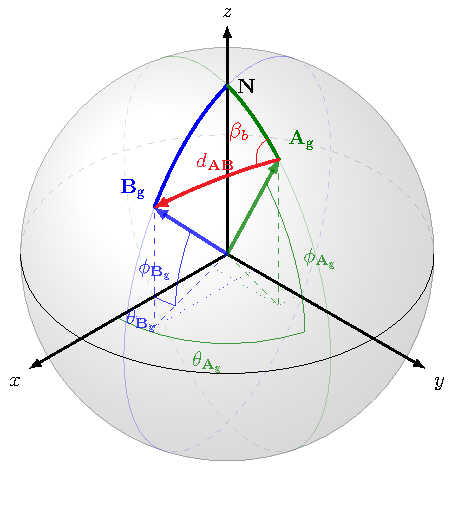
\includegraphics[width=0.95\textwidth]{../pictures/globo.pdf}
            \end{column}
            \begin{column}{0.45\textwidth}
                \begin{itemize}[<+(-3)->]\addtolength{\itemsep}{0.5\baselineskip}
                    \item \textcolor{Green}{$\mathbf{A}_\text{g}$} e \textcolor{Blue}{$\mathbf{B}_\text{g}$} são coordenadas geográficas
                    \item \textcolor{Green}{$\theta_{\mathbf{A}_\text{g}}$} e \textcolor{Blue}{$\theta_{\mathbf{B}_\text{g}}$} são latitudes
                    \item \textcolor{Green}{$\phi_{\mathbf{A}_\text{g}}$} e \textcolor{Blue}{$\phi_{\mathbf{B}_\text{g}}$} são longitudes
                    \item Conhecendo essas informações, é possível determinar o ângulo \textcolor{Red}{$\beta_b$} relativo entre as duas coordenadas
                    \item Também é possível determinar sua distância \textcolor{Red}{$d_\mathbf{AB}$}
                \end{itemize}
            \end{column}
        \end{columns}
    \end{frame}

% \subsection{Cálculo de Bearing}
%     \begin{frame}{Cálculo de Bearing}
%         % \begin{multicols}{2}
%             \begin{equation*}
%                 \Delta_\phi = \textcolor{Blue}{\phi_{\mathbf{B}_\text{g}}} - \textcolor{Green}{\phi_{\mathbf{A}_\text{g}}}
%             \end{equation*}
%             \begin{equation*}
%                 \Delta_\theta = \textcolor{Blue}{\theta_{\mathbf{B}_\text{g}}} - \textcolor{Green}{\theta_{\mathbf{A}_\text{g}}}
%             \end{equation*}
%             \begin{equation*}
%                 X = \cos\left(\textcolor{Blue}{\theta_{\mathbf{B}_\text{g}}}\right)\cdot \sin\left(\Delta_\phi\right)
%             \end{equation*}
%             \begin{equation*}
%                 Y = \cos\left(\textcolor{Green}{\theta_{\mathbf{A}_\text{g}}}\right)\cdot\sin\left(\textcolor{Blue}{\theta_{\mathbf{B}_\text{g}}}\right) - \sin\left(\textcolor{Green}{\theta_{\mathbf{A}_\text{g}}}\right) \cdot \cos\left(\textcolor{Green}{\theta_{\mathbf{B}_\text{g}}}\right) \cdot \cos\left(\Delta_\phi\right)
%             \end{equation*}
%             \begin{equation*}
%                 Z = \sin^2\left(\frac{\Delta_\theta}{2}\right) + \cos\left(\textcolor{Blue}{\theta_{\mathbf{B}_\text{g}}}\right) \cdot \cos\left(\textcolor{Green}{\theta_{\mathbf{A}_\text{g}}}\right) \cdot \sin^2\left(\frac{\Delta_\phi}{2}\right)
%             \end{equation*}
%             \begin{equation*}
%                 \textcolor{Red}{\beta_b} = \arctan\left(\frac{X}{Y}\right) - \frac{\pi}{2}
%             \end{equation*}
%             \begin{equation*}
%                 \textcolor{Red}{d_\mathbf{AB}} = R_\text{Terra} \cdot 2 \cdot \arctan\left(\frac{\sqrt{Z}}{\sqrt{1-Z}}\right)
%             \end{equation*}
%         % \end{multicols}
%     \end{frame}

\begin{frame}{Coordenadas Geográficas}
	\begin{itemize}[<+->]\addtolength{\itemsep}{0.5\baselineskip}
		\item É necessário decodificar os dados recebidos pela telemetria do foguete;
		\item A precisão da busca fica dependente da precisão do GNSS;
		\item O método baseia-se na ideia de que a equipe de busca tem acesso à própria coordenada geográfica;
		\item Num espaço sem acesso à internet, obter tal coordenada pode ser um problema;
		\item Se o sinal da telemetria for fraco, pode se tornar inviável utilizar este método.
	\end{itemize}
\end{frame}

    
\section{Emissão de sinais}

    \begin{frame}{Emissão de sinal radial}
        % % \begin{center}
\begin{circuitikz}[american, voltage shift=0.5, line width=0.5]
    % Variables
    \def\D{\N*\T}        
    \def\wavelength{1}
    \def\d{0.5*\wavelength}

    
    \begin{axis}[
        at={(0,0)},
        view={0}{90},
        hide axis,
        colormap={custom}{color=(white) color=(Gray)},
        trig format plots=rad,
        x=1cm,
        y=1cm,
        z=0cm,
    ]
    
    \clip[] (-0.5,-4) rectangle (13.1,4);
    \addplot3[
        data cs=polar,
        samples=25,
        domain=0:2*pi,
        domain y=0:15,
        samples y=100,
        surf,shader=interp,
    ] {sin(2*pi*y + 0.5*pi)};



    \coordinate (O) at (0,0);
    % \draw [help lines, dashed] (-5,-3) grid (5,3); % desenha grid
    % \draw [red] (O) node[draw,cross out] {}; % marca pont(0,0) 

    \draw[thick]
        (0,0) node[dinantenna]{}
    ;
        



    \end{axis}
        

\end{circuitikz}
% \end{center}
        
\includegraphics{../pictures/signal.pdf}
    \end{frame}

    \begin{frame}{Frentes de onda}
        % \begin{circuitikz}[american, voltage shift=0.5, line width=0.5]
    % Variables
    \def\T{1}
    \def\A{1}
    \def\N{5}
    \def\D{\N*\T}
    \def\wavelength{1}
    \def\d{0.5*\wavelength}


    \begin{axis}[
        at={(0,0)},
        view={0}{90},
        hide axis,
        colormap={custom}{color=(white) color=(Gray)},
        trig format plots=rad,
        x=1cm,
        y=1cm,
        z=0cm,
    ]
    \clip[] (-0.5,-4) rectangle (13.1,4);
    \addplot3[
        data cs=polar,
        samples=25,
        domain=0:2*pi,
        domain y=0:15,
        samples y=100,
        surf,shader=interp,
    ] {sin(2*pi*y/\wavelength + 0.5*pi)};



        \coordinate (O) at (0,0);
        % \draw [help lines, dashed] (-5,-3) grid (5,3); % desenha grid
        % \draw [red] (O) node[draw,cross out] {}; % marca pont(0,0)

        \draw[thick]
            (0,0) node[dinantenna]{}
        ;

        % \clip[] (-0.1,-4) rectangle (13.1,4);
        \pgfplotsinvokeforeach{1,2,...,13} {
        \draw [Black] (axis cs:0,0) circle (#1*\wavelength);
        }


    \end{axis}


\end{circuitikz}
        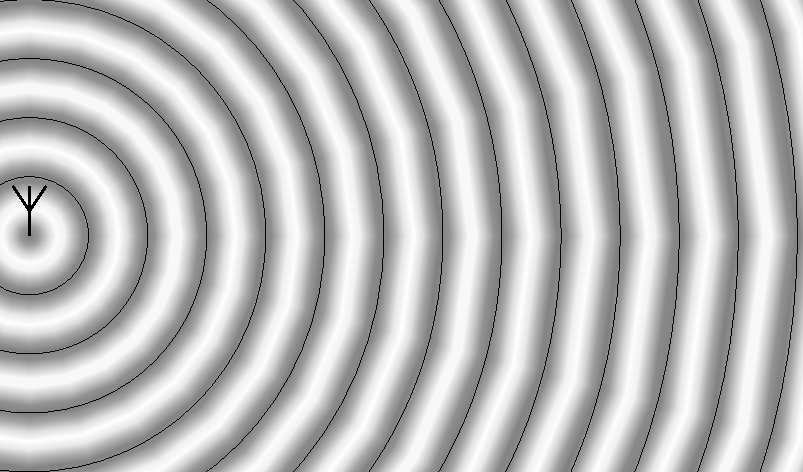
\includegraphics{../pictures/signal+lines.pdf}
    \end{frame}

    \begin{frame}{Representação de frentes de onda}
            \begin{circuitikz}[american, voltage shift=0.5, line width=0.5]

        \def\wavelength{1}
        \def\d{0.5*\wavelength}

        \coordinate (O) at (0,0);
        \coordinate (antenna) at (0,0);
        % \draw [help lines, dashed] (-5,-3) grid (5,3); % desenha grid
        % \draw [red] (O) node[draw,cross out] {}; % marca pont(0,0) 

        \draw[thick]
            (antenna) node[dinantenna]{}
        ;
        
        \clip[] (-0.5,-4) rectangle (13.1,4);
        \draw [gray, thin]
        \foreach \x in {1,2,...,13} {
            (antenna) circle (\x*\wavelength)
        }
        ;

        % \foreach \x in {0,60,...,300} {
        %     \draw[thick] (\x:1 cm) -- (\x + 60:1 cm);
            
        %     \draw (\x + 30:1.732 cm) node[Gray, circ]{};
        %     \draw[Gray, dashed] (\x:1 cm) -- ++(\x: 0.9cm);
        %     \draw[Gray, dotted]
        %     %     % (\x:1 cm) arc (\x+240:\x+180:1cm)
        %         (\x:1 cm) arc [start angle=\x+120, delta angle=110, radius=1cm]
        %         (\x:1 cm) arc [start angle=\x+120, delta angle=-50, radius=1cm]
        %     ;
        % }
    
        % \draw (0,0) node [circ] {} node [below left,font={\scriptsize\bfseries}] {BS};
        % \draw[thick, densely dotted] (0,0) circle (1cm);
        
        % \draw[-latex] (0,0) -- (0:1cm) node[midway, below] {$R_c$};
        % \draw[-latex] (0,0) -- (90:0.866cm) node[midway, left] {$R$};
            
    \end{circuitikz}

    \end{frame}

\subsection{Onda plana}

    \begin{frame}{Comportamento da onda no espaço próximo}
            % \resizebox{\textwidth}{!}{%
    \begin{circuitikz}[american, voltage shift=0.5, line width=0.5]

        \def\wavelength{0.5}
        \def\d{0.5*\wavelength}

        \def\closeRange{1}
        \def\farRange{\closeRange+30}

        \coordinate (O) at (0,0);
        \coordinate (antenna) at (-\closeRange,0);
        % \draw [help lines, dashed] (-5,-3) grid (5,3); % desenha grid
        % \draw [red] (O) node[draw,cross out] {}; % marca pont(0,0)

        \draw[thick]
            (antenna) node[dinantenna, scale=0.75]{}
        ;

        % \draw (\closeRange-0.5,-4) rectangle (\farRange+0.1,4);
        \clip (-0.75,-1.5) rectangle (12.1,1.5);
        \foreach \x [evaluate={\z=int((\x+\closeRange));}] in {0,...,30} {
            \draw [gray, thin, opacity=0.5] (antenna) circle (\z*\wavelength);
            \draw [black]
            (antenna) ++ (\z*\wavelength,0)
            node[anchor=south, font = {\footnotesize\bfseries}, rotate=-90,scale=0.75]{$\z\lambda$}
            ++(0, -4)
            -- ++(0,8);
        }

        \draw [Red, thick] (antenna) ++ (8*\wavelength,-4) -- ++(0,8);

        % \foreach \x in {0,60,...,300} {
        %     \draw[thick] (\x:1 cm) -- (\x + 60:1 cm);

        %     \draw (\x + 30:1.732 cm) node[Gray, circ]{};
        %     \draw[Gray, dashed] (\x:1 cm) -- ++(\x: 0.9cm);
        %     \draw[Gray, dotted]
        %     %     % (\x:1 cm) arc (\x+240:\x+180:1cm)
        %         (\x:1 cm) arc [start angle=\x+120, delta angle=110, radius=1cm]
        %         (\x:1 cm) arc [start angle=\x+120, delta angle=-50, radius=1cm]
        %     ;
        % }

        % \draw (0,0) node [circ] {} node [below left,font={\scriptsize\bfseries}] {BS};
        % \draw[thick, densely dotted] (0,0) circle (1cm);

        % \draw[-latex] (0,0) -- (0:1cm) node[midway, below] {$R_c$};
        % \draw[-latex] (0,0) -- (90:0.866cm) node[midway, left] {$R$};

    \end{circuitikz}
  % }

    \end{frame}

    \begin{frame}{Comportamento da onda em espaço distante (\textit{far field})}
        \resizebox{\textwidth}{!}{%
    \begin{circuitikz}[american, voltage shift=0.5, line width=0.5]

        \def\wavelength{0.75}
        \def\d{0.5*\wavelength}

        \def\closeRange{25}
        \def\farRange{\closeRange+20}

        \coordinate (O) at (0,0);
        \coordinate (antenna) at (-\closeRange*\wavelength,0);
        % \draw [help lines, dashed] (-5,-3) grid (5,3); % desenha grid
        % \draw [red] (O) node[draw,cross out] {}; % marca pont(0,0) 

        % \draw[thick]
        %     (antenna) node[dinantenna]{}
        % ;
        
        % \draw (-0.5,-1.5) rectangle (13.1,1.5);
        \clip (-0.5,-1.5) rectangle (13.1,1.5);
        \foreach \x [evaluate={\z=int((\x+\closeRange));}] in {0,...,20} {
            \draw [black, thick] 
            (antenna) ++ (\z*\wavelength,0) 
            node[anchor=south, font = {\footnotesize\bfseries}, rotate=-90]{$\z\lambda$}
            ++(0, -4) 
            -- ++(0,8);
            \draw [gray, thin] (antenna) circle (\z*\wavelength);
        }


        % \foreach \x in {0,60,...,300} {
        %     \draw[thick] (\x:1 cm) -- (\x + 60:1 cm);
            
        %     \draw (\x + 30:1.732 cm) node[Gray, circ]{};
        %     \draw[Gray, dashed] (\x:1 cm) -- ++(\x: 0.9cm);
        %     \draw[Gray, dotted]
        %     %     % (\x:1 cm) arc (\x+240:\x+180:1cm)
        %         (\x:1 cm) arc [start angle=\x+120, delta angle=110, radius=1cm]
        %         (\x:1 cm) arc [start angle=\x+120, delta angle=-50, radius=1cm]
        %     ;
        % }
    
        % \draw (0,0) node [circ] {} node [below left,font={\scriptsize\bfseries}] {BS};
        % \draw[thick, densely dotted] (0,0) circle (1cm);
        
        % \draw[-latex] (0,0) -- (0:1cm) node[midway, below] {$R_c$};
        % \draw[-latex] (0,0) -- (90:0.866cm) node[midway, left] {$R$};
            
    \end{circuitikz}
}



% \begin{center}
%     % \resizebox{\textwidth}{!}{%
%     \begin{circuitikz}[american, voltage shift=0.5, line width=0.5]

%         \def\wavelength{1}
%         \def\d{0.5*\wavelength}

        
%         \def\closeRange{-50}
%         \def\closeRangePlus{\closeRange+1}
%         \def\farRange{\closeRange+13}

%         \coordinate (O) at (0,0);
%         \coordinate (antenna) at (\closeRange,0);
%         % \draw [help lines, dashed] (-5,-3) grid (5,3); % desenha grid
%         % \draw [red] (O) node[draw,cross out] {}; % marca pont(0,0) 

%         % \draw[thick]
%         %     (antenna) node[dinantenna]{}
%         % ;
        
%         % \draw (\closeRange-0.5,-4) rectangle (\farRange+0.1,4);
%         \clip (-0.5,-4) rectangle (13.1,4);
%         \foreach \x in {0,...,13} {
%         \draw [black, thick] (antenna) ++ ({(\x-\closeRange)*\wavelength}, -4) -- ++(0,8);
%         \draw [gray, thin] (antenna) circle ({(\x-\closeRange)*\wavelength});
%         }

%         % \foreach \x in {0,60,...,300} {
%         %     \draw[thick] (\x:1 cm) -- (\x + 60:1 cm);
            
%         %     \draw (\x + 30:1.732 cm) node[Gray, circ]{};
%         %     \draw[Gray, dashed] (\x:1 cm) -- ++(\x: 0.9cm);
%         %     \draw[Gray, dotted]
%         %     %     % (\x:1 cm) arc (\x+240:\x+180:1cm)
%         %         (\x:1 cm) arc [start angle=\x+120, delta angle=110, radius=1cm]
%         %         (\x:1 cm) arc [start angle=\x+120, delta angle=-50, radius=1cm]
%         %     ;
%         % }
    
%         % \draw (0,0) node [circ] {} node [below left,font={\scriptsize\bfseries}] {BS};
%         % \draw[thick, densely dotted] (0,0) circle (1cm);
        
%         % \draw[-latex] (0,0) -- (0:1cm) node[midway, below] {$R_c$};
%         % \draw[-latex] (0,0) -- (90:0.866cm) node[midway, left] {$R$};
            
%     \end{circuitikz}
%   % }
% \end{center}

    \end{frame}
    \section{AoA}

    \begin{frame}{\textit{Angle of Arrival}}
        % % \resizebox{!}{0.7\textheight}{%
\begin{circuitikz}[american, voltage shift=0.5, line width=0.5, every node/.style={font = {\footnotesize\bfseries}}]

    \def\wavelength{3.5}
    \pgfmathsetmacro\d{0.5*\wavelength}

    \def\antennaAngle{20}
    \pgfmathsetmacro\signalAngle{\antennaAngle+40}

    \def\closeRange{9}
    \def\farRange{\closeRange+13}

	\def\NAntennas{3}
	\pgfmathsetmacro\AngleAntennas{360/\NAntennas}
	\def\ShiftAngleAntennas{-90}

	\pgfmathsetmacro\RhoAntennas{\d/(2*sin(180/\NAntennas))}

    \def\centerarc(#1)(#2:#3:#4)% Syntax: [draw options] (center) (initial angle:final angle:radius)
    { ($(#1)+({#4*cos(#2)},{#4*sin(#2)})$) arc (#2:#3:#4) }

    \def\coordref[#1](#2){%

        \coordinate(sysref) at (#2);

        \draw[#1, -latex] (sysref) ++(-0.4,-0.3) -- ++(0.9,0) node[midway, below]{$x$};
        \draw[#1, -latex] (sysref) ++(-0.3,-0.4) -- ++(0,0.9) node[midway, left]{$y$};
        \draw[#1, -latex] \centerarc(sysref)(-90:180:0.25);
        \draw[#1] (sysref) node{$+$}
    }

    \coordinate (bottomleft) at (-3.5,-1);
    \coordinate (topright) at (3.5,5);


    % \draw[Red,dashed] (bottomleft) rectangle (topright);
    \clip (bottomleft) rectangle (topright);

    \coordinate (O) at (0,0);
    \coordinate (sourceAntenna) at (\signalAngle:\closeRange*\wavelength);
    % \draw [help lines, dashed] (bottomleft) grid (topright); % desenha grid
    % \draw [red] (O) node[draw,cross out] {}; % marca pont(0,0)

    % Circulo de antenas
	% \draw[densely dotted, opacity=0.25] (O) ++(90:\RhoAntennas) circle (\RhoAntennas);

    % Linhas do sinal de fundo
    \foreach \x [evaluate={\y=int((\x+\closeRange));\z=int((\x+\closeRange));}] in {-3,...,3} {
        \draw [black!75, very thin]
        (sourceAntenna) ++ (\signalAngle:-\z*\wavelength)
            % node[anchor=west, font = {\footnotesize\bfseries}]{$\y\lambda$}
        ($(sourceAntenna) + (\signalAngle:-\z*\wavelength) + ({10*cos(\signalAngle+90)},{10*sin(\signalAngle+90)})$)
            --
        ($(sourceAntenna) + (\signalAngle:-\z*\wavelength) - ({10*cos(\signalAngle+90)},{10*sin(\signalAngle+90)})$)
        % \draw [gray, thin] (sourceAntenna) circle (\z)
        ;
    }

    % Antenas
    \draw[thick, cmyk_R] (O) node[dinantenna] (A00) {} ;
    % \draw[thick, cmyk_G, opacity=0.75] (O) ++(60:\d) node[dinantenna] (A0d) {} node [below] {$A_{k+2}$};
    \draw[thick, cmyk_B] (O) ++(\antennaAngle:\d) node[dinantenna] (Ad0) {} ;

    \draw[very thin, Black!50, -latex] % Desenha eixo X
        (-3,0) -- (3,0) node[below left] {$x$}
    ;

    % Ângulo alpha entre antenas
    \draw[thin, cmyk_M]
        \centerarc(O)(0:\antennaAngle:0.3)
        node [above, inner sep=3pt] {$\alpha$}
    ;


    % Desenha senoide de fundo
    \draw[Goldenrod, domain=-8:8, samples=100]
        (A00) ++(\signalAngle+90:0.5*\wavelength) coordinate(signalAux)
        plot[shift={(signalAux)}, rotate=\signalAngle]({\x},{cos(\x * pi * 2 / \wavelength r)})
    ;

    % Direção do sinal
    \draw[very thick, dashed, -latex, Goldenrod]
        % (A00) ++(1.5*\d,0) ++ (\signalAngle:-0.5*\d) -- coordinate(angleArrow) ++(\signalAngle:\d)
        (A00) ++(-2,0) ++ (\signalAngle:-0.25*\d) -- coordinate(angleArrow) ++ (\signalAngle:0.5*\d) --++(\signalAngle:0.25*\d)
    ;
    % Angulo Theta do sinal
    \draw[thin]
        (angleArrow) ++ (0.4, 0) node [below,inner sep=2pt] {$\theta_\text{\ac{AoA}}$}
        \centerarc(angleArrow)(0:\signalAngle:0.4)
    ;

    % Triangulo retângulo + quadradinho
    \draw[Black]

        (A00) --++($({\signalAngle-90}:{\d*sin(\signalAngle-\antennaAngle)})$) coordinate (pontoTriangulo) -- (Ad0) -- (A00)

        (pontoTriangulo)
          ++(\signalAngle:0.125)
        --++(\signalAngle+90:0.125)
        --++(\signalAngle+180:0.125)
    ;

    % Arco do angulo beta
    \draw[thin, Purple]
        (Ad0) ++ (180+\antennaAngle:0.4) node[above, inner sep=3pt] {$\beta$}
        \centerarc(Ad0)(180+\antennaAngle:180+\signalAngle:0.4)
    ;

    % Distânci d entre antenas
    \draw[latex-latex]
        ($(A00)+(0,1)$) -- ($(Ad0)+(0,1)$) node [midway, fill=white, circle, inner sep=1pt] {$d$}
    ;

    \newcommand\CircleRadius{3cm}
    %   \draw (0,0) circle (\CircleRadius);
    % special method of noting the position of a point
    \coordinate (P) at (50:\CircleRadius);

\end{circuitikz}
% }


        \centering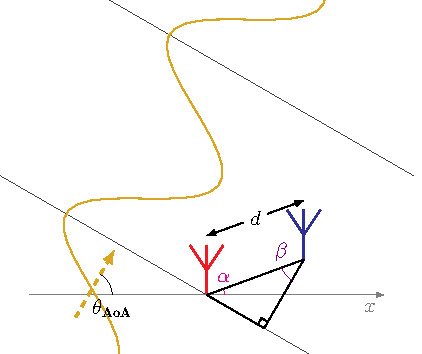
\includegraphics{../pictures/AoA_1_new}
    \end{frame}

    \begin{frame}{\textit{Angle of Arrival}}
        %     % \resizebox{!}{0.7\textheight}{%
    \begin{circuitikz}[american, voltage shift=0.5, line width=0.5,every node/.style={font = {\footnotesize\bfseries}}]

        \def\wavelength{3.5}
        \def\d{0.5*\wavelength}

        \def\antennaAngle{210}

        \def\closeRange{9}
        \def\farRange{\closeRange+13}

        \def\centerarc[#1](#2)(#3:#4:#5)% Syntax: [draw options] (center) (initial angle:final angle:radius)
        { \draw[#1] ($(#2)+({#5*cos(#3)},{#5*sin(#3)})$) arc (#3:#4:#5) node[midway,anchor=west] {$\beta$}; }


        \coordinate (O) at (0,0);
        \coordinate (antenna) at (\antennaAngle:\closeRange*\wavelength);
        % \draw [help lines, dashed] (-5,-3) grid (5,3); % desenha grid
        % \draw [red] (O) node[draw,cross out] {}; % marca pont(0,0) 
        
        % \draw (-6.8,-4) rectangle (6.8,4);
        \clip (-3.5,-3.5) rectangle (3.5,3.5);

        % \draw[thick]
        %     (antenna) node[dinantenna]{}
        % ;
        
        \foreach \x [evaluate={\y=int((\x+\closeRange));\z=int((\x+\closeRange));}] in {-3,...,3} {
            \draw [black, thin] 
            (antenna) ++ (\antennaAngle:-\z*\wavelength)
                % node[anchor=west, font = {\footnotesize\bfseries}]{$\y\lambda$}
            ($(antenna) + (\antennaAngle:-\z*\wavelength) + ({10*cos(\antennaAngle+90)},{10*sin(\antennaAngle+90)})$)
                -- 
            ($(antenna) + (\antennaAngle:-\z*\wavelength) - ({10*cos(\antennaAngle+90)},{10*sin(\antennaAngle+90)})$);
            % \draw [gray, thin] (antenna) circle (\z);
        }
        
        \draw[thick]
            (0,0)  node[Green, dinantenna] (A00) {}
            % (0,\d) node[Blue,  dinantenna] (A0d) {}
            (\d,0) node[Red,   dinantenna] (Ad0) {}
        ;

        \draw[very thick, dashed, -latex]
            (A00) ++(-\d,0) coordinate(aux) ++(\antennaAngle:0.5*\d) -- ++(\antennaAngle:-\d)
        ;

        
        \draw[Goldenrod, domain=-8:8, samples=100] plot[shift={(aux)}, rotate=\antennaAngle]({\x},{sin(\x * pi * 2 / \wavelength r)});
        
        \draw[thin, opacity=0.5]
            (A00) ++ ($({\antennaAngle-90}:{\d*sin(\antennaAngle)})$) -- (Ad0) -- (A00)

            ($({\antennaAngle-90}:{\d*sin(\antennaAngle)})$) 
              ++(\antennaAngle+180:0.125)
            --++(\antennaAngle-90:0.125)
            --++(\antennaAngle:0.125)

            
        ;

        \centerarc[thin, opacity=0.5](A00)(\antennaAngle+90:360:0.4)

        \draw[latex-latex]
            ($(A00)+(0,1)$) -- ($(Ad0)+(0,1)$) node [midway, fill=white] {$d$}
        ;
        


        % \foreach \x in {0,60,...,300} {
        %     \draw[thick] (\x:1 cm) -- (\x + 60:1 cm);
            
        %     \draw (\x + 30:1.732 cm) node[Gray, circ]{};
        %     \draw[Gray, dashed] (\x:1 cm) -- ++(\x: 0.9cm);
        %     \draw[Gray, dotted]
        %     %     % (\x:1 cm) arc (\x+240:\x+180:1cm)
        %         (\x:1 cm) arc [start angle=\x+120, delta angle=110, radius=1cm]
        %         (\x:1 cm) arc [start angle=\x+120, delta angle=-50, radius=1cm]
        %     ;
        % }
    
        % \draw (0,0) node [circ] {} node [below left,font={\scriptsize\bfseries}] {BS};
        % \draw[thick, densely dotted] (0,0) circle (1cm);
        
        % \draw[-latex] (0,0) -- (0:1cm) node[midway, below] {$R_c$};
        % \draw[-latex] (0,0) -- (90:0.866cm) node[midway, left] {$R$};
            
    \end{circuitikz}
  % }


        \centering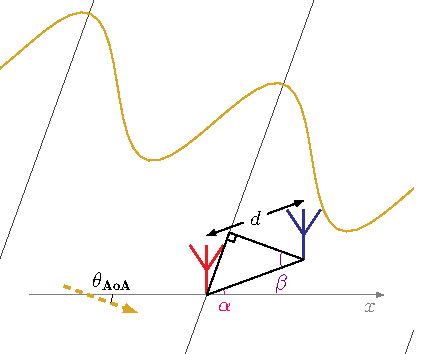
\includegraphics{../pictures/AoA_2_new}
    \end{frame}

    \begin{frame}{\textit{Angle of Arrival}}
        %     % \resizebox{!}{0.7\textheight}{%
    \begin{circuitikz}[american, voltage shift=0.5, line width=0.5,every node/.style={font = {\footnotesize\bfseries}}]

        \def\wavelength{3.5}
        \def\d{0.5*\wavelength}


        \def\antennaAngle{180}
        \def\closeRange{9}
        \def\farRange{\closeRange+13}

        \def\centerarc[#1](#2)(#3:#4:#5)% Syntax: [draw options] (center) (initial angle:final angle:radius)
        { \draw[#1] ($(#2)+({#5*cos(#3)},{#5*sin(#3)})$) arc (#3:#4:#5) node[midway,anchor=west] {$\beta$}; }


        \coordinate (O) at (0,0);
        \coordinate (antenna) at (\antennaAngle:\closeRange*\wavelength);
        % \draw [help lines, dashed] (-5,-3) grid (5,3); % desenha grid
        % \draw [red] (O) node[draw,cross out] {}; % marca pont(0,0) 
        
        % \draw (-6.8,-4) rectangle (6.8,4);
        \clip (-3.5,-3.5) rectangle (3.5,3.5);

        % \draw[thick]
        %     (antenna) node[dinantenna]{}
        % ;
        
        \foreach \x [evaluate={\y=int((\x+\closeRange));\z=int((\x+\closeRange));}] in {-3,...,3} {
            \draw [black, thin] 
            (antenna) ++ (\antennaAngle:-\z*\wavelength)
                % node[anchor=west, font = {\footnotesize\bfseries}]{$\y\lambda$}
            ($(antenna) + (\antennaAngle:-\z*\wavelength) + ({10*cos(\antennaAngle+90)},{10*sin(\antennaAngle+90)})$)
                -- 
            ($(antenna) + (\antennaAngle:-\z*\wavelength) - ({10*cos(\antennaAngle+90)},{10*sin(\antennaAngle+90)})$);
            % \draw [gray, thin] (antenna) circle (\z);
        }
        
        \draw[thick]
            (0,0)  node[Green, dinantenna] (A00) {}
            % (0,\d) node[Blue,  dinantenna] (A0d) {}
            (\d,0) node[Red,   dinantenna] (Ad0) {}
        ;

        \draw[very thick, dashed, -latex]
            (A00) ++(-\d,0) coordinate(aux) ++(\antennaAngle:0.5*\d) -- ++(\antennaAngle:-\d)
        ;

        
        \draw[Goldenrod, domain=-8:8, samples=100] plot[shift={(aux)}, rotate=\antennaAngle]({\x},{cos(\x * pi * 2 / \wavelength r)});
        % \draw[thin, densely dotted]
        %     (A00) ++ ($({\antennaAngle-90}:{\d*sin(\antennaAngle)})$) -- (Ad0) -- (A00)

        %     ($({\antennaAngle-90}:{\d*sin(\antennaAngle)})$) 
        %       ++(\antennaAngle+180:0.25)
        %     --++(\antennaAngle-90:0.25)
        %     --++(\antennaAngle:0.25)

            
        % ;

        % \centerarc[thin, densely dotted](A00)(\antennaAngle+90:360:0.4)

        \draw[latex-latex]
            ($(A00)+(0,1)$) -- ($(Ad0)+(0,1)$) node [midway, fill=white] {$d$}
        ;

        % \draw[color=Blue, samples=100, domain=-4:4, smooth]
        %     (A00)++(-\d,0)
        %     % plot[rotate=\antennaAngle] ({\x},{sin((\x r)*0.31830)})
        % ;


        % \foreach \x in {0,60,...,300} {
        %     \draw[thick] (\x:1 cm) -- (\x + 60:1 cm);
            
        %     \draw (\x + 30:1.732 cm) node[Gray, circ]{};
        %     \draw[Gray, dashed] (\x:1 cm) -- ++(\x: 0.9cm);
        %     \draw[Gray, dotted]
        %     %     % (\x:1 cm) arc (\x+240:\x+180:1cm)
        %         (\x:1 cm) arc [start angle=\x+120, delta angle=110, radius=1cm]
        %         (\x:1 cm) arc [start angle=\x+120, delta angle=-50, radius=1cm]
        %     ;
        % }
    
        % \draw (0,0) node [circ] {} node [below left,font={\scriptsize\bfseries}] {BS};
        % \draw[thick, densely dotted] (0,0) circle (1cm);
        
        % \draw[-latex] (0,0) -- (0:1cm) node[midway, below] {$R_c$};
        % \draw[-latex] (0,0) -- (90:0.866cm) node[midway, left] {$R$};
            
    \end{circuitikz}
  % }


        \centering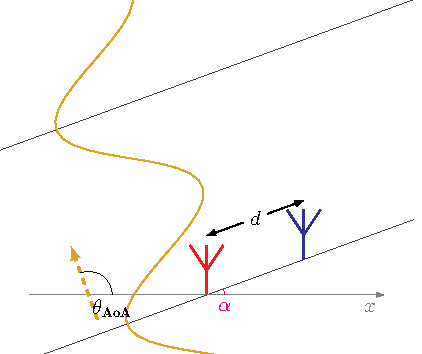
\includegraphics{../pictures/AoA_3_new}
    \end{frame}

    \begin{frame}{\textit{Angle of Arrival}}
        % % \resizebox{!}{0.7\textheight}{%
\begin{circuitikz}[american, voltage shift=0.5, line width=0.5, every node/.style={font = {\footnotesize\bfseries}}]

    \def\wavelength{3.5}
    \pgfmathsetmacro\d{0.5*\wavelength}

    \def\antennaAngle{20}
    \def\signalAngle{\antennaAngle}

    \def\closeRange{9}
    \def\farRange{\closeRange+13}

	\def\NAntennas{3}
	\pgfmathsetmacro\AngleAntennas{360/\NAntennas}
	\def\ShiftAngleAntennas{-90}

	\pgfmathsetmacro\RhoAntennas{\d/(2*sin(180/\NAntennas))}

    \def\centerarc(#1)(#2:#3:#4)% Syntax: [draw options] (center) (initial angle:final angle:radius)
    { ($(#1)+({#4*cos(#2)},{#4*sin(#2)})$) arc (#2:#3:#4) }

    \def\coordref[#1](#2){%

        \coordinate(sysref) at (#2);

        \draw[#1, -latex] (sysref) ++(-0.4,-0.3) -- ++(0.9,0) node[midway, below]{$x$};
        \draw[#1, -latex] (sysref) ++(-0.3,-0.4) -- ++(0,0.9) node[midway, left]{$y$};
        \draw[#1, -latex] \centerarc(sysref)(-90:180:0.25);
        \draw[#1] (sysref) node{$+$}
    }

    \coordinate (bottomleft) at (-3.5,-1);
    \coordinate (topright) at (3.5,5);


    % \draw[Red,dashed] (bottomleft) rectangle (topright);
    \clip (bottomleft) rectangle (topright);

    \coordinate (O) at (0,0);
    \coordinate (sourceAntenna) at (\signalAngle:\closeRange*\wavelength);
    % \draw [help lines, dashed] (bottomleft) grid (topright); % desenha grid
    % \draw [red] (O) node[draw,cross out] {}; % marca pont(0,0)

    % Circulo de antenas
	% \draw[densely dotted, opacity=0.25] (O) ++(90:\RhoAntennas) circle (\RhoAntennas);

    % Linhas do sinal de fundo
    \foreach \x [evaluate={\y=int((\x+\closeRange));\z=int((\x+\closeRange));}] in {-3,...,3} {
        \draw [black!75, very thin]
        (sourceAntenna) ++ (\signalAngle:-\z*\wavelength)
            % node[anchor=west, font = {\footnotesize\bfseries}]{$\y\lambda$}
        ($(sourceAntenna) + (\signalAngle:-\z*\wavelength) + ({10*cos(\signalAngle+90)},{10*sin(\signalAngle+90)})$)
            --
        ($(sourceAntenna) + (\signalAngle:-\z*\wavelength) - ({10*cos(\signalAngle+90)},{10*sin(\signalAngle+90)})$)
        % \draw [gray, thin] (sourceAntenna) circle (\z)
        ;
    }

    % Antenas
    \draw[thick, cmyk_R] (O) node[dinantenna] (A00) {} ;
    % \draw[thick, cmyk_G, opacity=0.75] (O) ++(60:\d) node[dinantenna] (A0d) {} node [below] {$A_{k+2}$};
    \draw[thick, cmyk_B] (O) ++(\antennaAngle:\d) node[dinantenna] (Ad0) {} ;

    \draw[very thin, Black!50, -latex] % Desenha eixo X
        (-3,0) -- (3,0) node[below left] {$x$}
    ;

    % Ângulo alpha entre antenas
    \draw[thin, cmyk_M]
		(0.3,0) node [below, inner sep=3pt] {$\alpha$}
		\centerarc(O)(0:\antennaAngle:0.3)
    ;


    % Desenha senoide de fundo
    \draw[Goldenrod, domain=-8:8, samples=100]
        (A00) ++(\signalAngle+90:0.75*\wavelength) coordinate(signalAux)
        plot[shift={(signalAux)}, rotate=\signalAngle]({\x},{cos(\x * pi * 2 / \wavelength r)})
    ;

    % Direção do sinal
    \draw[very thick, dashed, -latex, Goldenrod]
        % (A00) ++(1.5*\d,0) ++ (\signalAngle:-0.25*\d) -- coordinate(angleArrow) ++(\signalAngle:0.85*\d)
        (A00) ++(-2,0) ++ (\signalAngle:-0.25*\d) -- coordinate(angleArrow) ++ (\signalAngle:0.5*\d) --++(\signalAngle:0.25*\d)
    ;
    % Angulo Theta do sinal
    \draw[thin]
        (angleArrow) ++ (0.4, 0) node [below,inner sep=2pt] {$\theta_\text{\ac{AoA}}$}
        \centerarc(angleArrow)(0:\signalAngle:0.4)
    ;

    % Triangulo retângulo + quadradinho
    \draw[Black]

    %     % (A00) --++($({\signalAngle-90}:{\d*sin(\signalAngle-\antennaAngle)})$) coordinate (pontoTriangulo) --
		(Ad0) -- (A00)

    %     % (pontoTriangulo)
    %     %   ++(\signalAngle:0.125)
    %     % --++(\signalAngle+90:0.125)
    %     % --++(\signalAngle+180:0.125)
    ;

    % % Arco do angulo beta
    % \draw[thin]
    %     \centerarc(Ad0)(180+\antennaAngle:180+\signalAngle:0.4) node[below, inner sep=3pt] {$\beta$}
    % ;

    % Distânci d entre antenas
    \draw[latex-latex]
        ($(A00)+(0,1)$) -- ($(Ad0)+(0,1)$) node [midway, fill=white, circle, inner sep=1pt] {$d$}
    ;

    \newcommand\CircleRadius{3cm}
    %   \draw (0,0) circle (\CircleRadius);
    % special method of noting the position of a point
    \coordinate (P) at (50:\CircleRadius);

\end{circuitikz}
% }


        \centering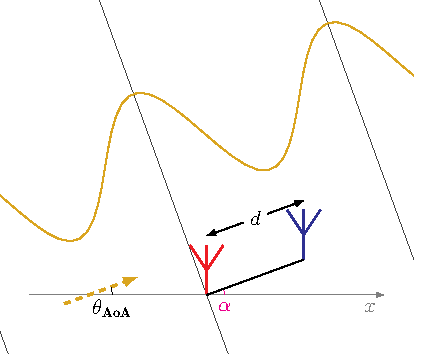
\includegraphics{../pictures/AoA_4_new}
    \end{frame}

    \begin{frame}{Distância $d$}
                \begin{columns}
            \begin{column}{0.45\textwidth}
                \centering \vfill
                    % \resizebox{!}{0.7\textheight}{%
    \begin{circuitikz}[american, voltage shift=0.5, line width=0.5,every node/.style={font = {\footnotesize\bfseries}}]

        \def\wavelength{4}
        \def\d{0.5*\wavelength}


        \def\antennaAngle{120}
        \def\closeRange{9}
        \def\farRange{\closeRange+13}

        \def\centerarc[#1](#2)(#3:#4:#5)% Syntax: [draw options] (center) (initial angle:final angle:radius)
        { \draw[#1] ($(#2)+({#5*cos(#3)},{#5*sin(#3)})$) arc (#3:#4:#5) node[midway,anchor=west] {$\beta$}; }


        \coordinate (O) at (0,0);
        \coordinate (antenna) at (\antennaAngle:\closeRange*\wavelength);
        % \draw [help lines, dashed] (-3,-3) grid (3,3); % desenha grid
        % \draw [red] (O) node[draw,cross out] {}; % marca pont(0,0) 
        
        % \draw (5,1.25) rectangle (-1,-1.1);
        \clip (5,1.25) rectangle (-1,-1.1);

        
        % \draw[Goldenrod, domain=-3:3, samples=100] plot[shift={(-1,-1)}, rotate=30]({\x},{sin(\x * pi * 2 / \wavelength r)});
        \draw[Goldenrod, domain=-3:6, samples=50] 
            plot ({\x},{cos(\x * pi * 2 / \wavelength r)})
        ;
        
        \draw[Black, dashed, domain=-3:6, samples=2] 
            plot[Black, thin, dashed, samples=2] (\x,0)
        ;
        
        
        % \pause
        \draw[thick]
            (0,0)  node[Green, dinantenna] (A00) {}
            % (0,\d) node[Blue,  dinantenna] (A0d) {}
            % (\d,0) node[Red,   dinantenna] (Ad0) {}
        ;
        
        % \pause
        \draw[thick]
            % (0,0)  node[Green, dinantenna] (A00) {}
            % (0,\d) node[Blue,  dinantenna] (A0d) {}
            (\d,0) node[Red,   dinantenna] (Ad0) {}
        ;

        \draw[latex-latex]
            ($(A00)+(0,1.1)$) -- ++(\wavelength,0) node [midway, fill=white] {$\lambda$}
        ;
    % \visible<7->{
        \draw[latex-latex]
            ($(A00)+(0,-0.1)$) -- ++(0.5*\wavelength,0) node [midway, fill=white, fill opacity=0.75, anchor=north] {$d = \sfrac{\lambda}{2}$}
        ;
    % }
            
    \end{circuitikz}
  % }\vfill
                \visible<5->{    % \resizebox{!}{0.7\textheight}{%
    \begin{circuitikz}[american, voltage shift=0.5, line width=0.5,every node/.style={font = {\footnotesize\bfseries}}]

        \def\wavelength{4}
        \def\d{0.5*\wavelength}


        \def\antennaAngle{120}
        \def\closeRange{9}
        \def\farRange{\closeRange+13}

        \def\centerarc[#1](#2)(#3:#4:#5)% Syntax: [draw options] (center) (initial angle:final angle:radius)
        { \draw[#1] ($(#2)+({#5*cos(#3)},{#5*sin(#3)})$) arc (#3:#4:#5) node[midway,anchor=west] {$\beta$}; }


        \coordinate (O) at (0,0);
        \coordinate (antenna) at (\antennaAngle:\closeRange*\wavelength);
        % \draw [help lines, dashed] (-3,-3) grid (3,3); % desenha grid
        % \draw [red] (O) node[draw,cross out] {}; % marca pont(0,0)

        % \draw (-6.8,-4) rectangle (6.8,4);
        \clip (-1,-1.1) rectangle (5,1.1);


        \draw[thick]
            (0,0)  node[cmyk_B, dinantenna] (A00) {}
            % (0,\d) node[Blue,  dinantenna] (A0d) {}
            (1.2*\d,0) node[cmyk_R,   dinantenna] (Ad0) {}
            (0.8*\d,0) node[cmyk_R,   dinantenna, opacity=0.2] (Ad0_phantom) {}
        ;

        % \draw[Goldenrod, domain=-3:3, samples=100] plot[shift={(-1,-1)}, rotate=30]({\x},{sin(\x * pi * 2 / \wavelength r)});
        \draw[Goldenrod, domain=-3:6, samples=50]
            plot ({\x},{cos(\x * pi * 2 / \wavelength r)})
        ;

        \draw[Black, dashed, domain=-3:6, samples=2]
            plot[Black, thin, dashed, samples=2] (\x,0)
        ;

        \draw [densely dotted, cmyk_R]
            (Ad0_phantom) --
            ++(0,{cos(1.2*\d * pi * 2 / \wavelength r)}) --
            ++({0.4*\d},0) --
            (Ad0)
        ;

    \end{circuitikz}
  % }}\vfill
                \visible<6->{    % \resizebox{!}{0.7\textheight}{%
    \begin{circuitikz}[american, voltage shift=0.5, line width=0.5,every node/.style={font = {\footnotesize\bfseries}}]

        \def\wavelength{4}
        \def\d{0.5*\wavelength}

        \def\centerarc[#1](#2)(#3:#4:#5)% Syntax: [draw options] (center) (initial angle:final angle:radius)
        { \draw[#1] ($(#2)+({#5*cos(#3)},{#5*sin(#3)})$) arc (#3:#4:#5) node[midway,anchor=west] {$\beta$}; }

        \coordinate (bottomleft) at (-1,-1.25);
        \coordinate (topright) at (5,1.1);

        % \draw[Red,dashed] (bottomleft) rectangle (topright);
        \clip (bottomleft) rectangle (topright);

        \coordinate (O) at (0,0);
        % \draw [help lines, dashed] (bottomleft) grid (topright); % desenha grid
        % \draw [red] (O) node[draw,cross out] {}; % marca pont(0,0)

        \pgfmathsetmacro\vCos{-cos(-0.5*pi*2/\wavelength r)}

        \draw[thick]
            (2,0)  node[cmyk_B, dinantenna] (A00) {}
            % (0,\d) node[Blue,  dinantenna] (A0d) {}
            (0.5,0) node[cmyk_R,   dinantenna] (Ad0) {}
            % (3.5,0) node[cmyk_R,   dinantenna, opacity=0.2] (Ad0_phantom) {}
        ;

        % \draw[Goldenrod, domain=-3:3, samples=100] plot[shift={(-1,-1)}, rotate=30]({\x},{sin(\x * pi * 2 / \wavelength r)});
        \draw[Goldenrod, domain=-3:6, samples=50]
            plot ({\x},{-cos(\x * pi * 2 / \wavelength r)})
        ;

        \draw[Black, dashed, domain=-3:6, samples=2]
            plot[Black, thin, dashed, samples=2] (\x,0)
        ;

    \end{circuitikz}
  % }}\vfill
            \end{column}
            \begin{column}{0.55\textwidth}
                \begin{itemize}[<+(-1)->]
                    \item Toma-se uma \textcolor{cmyk_B}{antena} como referência
                    \item Posiciona-se uma segunda \textcolor{Red}{antena} a uma distância determinada
                    \item Analisando a defasagem entre as antenas, é possível determinar o ângulo de incidência do sinal
                    \item Se a distância for maior que $\sfrac{\lambda}{2}$, haverá conflito de defasagem
                    \item Se for menor, há perda de resolução
                    \item Adota-se a distância de $d = \sfrac{\lambda}{2}$
                \end{itemize}
            \end{column}
        \end{columns}
    \end{frame}

\subsection{Malha de antenas}
    \begin{frame}{Geometria da malha de antenas}

        \begin{equation*}
            \rho = \frac{d}{2\cdot \sin\left(\displaystyle\frac{\pi}{N_\text{ant}}\right)}
        \end{equation*}

        \begin{equation*}
            k = \left\{1, 2, \dotsc, N_\text{ant}\right\}
        \end{equation*}

        \begin{equation*}
            \textcolor{cmyk_B}{A_k} =
            \rho
            \cdot \exp\left(\imath\cdot k \cdot \frac{2\pi}{N_\text{ant}}\right) =
            \left( \operatorname{\mathcal{Re}}\left( \textcolor{cmyk_B}{A_k} \right), ~\operatorname{\mathcal{Im}}\left( \textcolor{cmyk_B}{A_k} \right) \right) =
            \left( x_{A_k}, ~ y_{A_k} \right)
        \end{equation*}

        \begin{equation*}
            \textcolor{cmyk_M}{\alpha_k} = \arg\left( \textcolor{cmyk_B}{A_k} - \textcolor{cmyk_R}{A_{k+1}} \right)
        \end{equation*}
    \end{frame}

    \begin{frame}{Três antenas}
        \centering%
        % \fbox{%
            % \scalebox{0.75}%
            % \resizebox{0.5\textwidth}{!}
            % {% \resizebox{!}{0.7\textheight}{%
\begin{circuitikz}[american, voltage shift=0.5, line width=0.5,every node/.style={font = {\footnotesize\bfseries}}]

    \def\wavelength{8}
    \pgfmathsetmacro\d{0.5*\wavelength}

    \def\signalAngle{75}
    \def\antennaAngle{120}

    \def\closeRange{9}
    \def\farRange{\closeRange+13}

	\def\NAntennas{3}
	\pgfmathsetmacro\AngleAntennas{360/\NAntennas}
	\def\ShiftAngleAntennas{-90}

	\pgfmathsetmacro\RhoAntennas{\d/(2*sin(180/\NAntennas))}

    \def\centerarc(#1)(#2:#3:#4)% Syntax: [draw options] (center) (initial angle:final angle:radius)
    { ($(#1)+({#4*cos(#2)},{#4*sin(#2)})$) arc (#2:#3:#4) }

    \def\coordref[#1](#2){%

        \coordinate(sysref) at (#2);

        \draw[#1, -latex] (sysref) ++(-0.4,-0.3) -- ++(0.9,0) node[midway, below]{$x$};
        \draw[#1, -latex] (sysref) ++(-0.3,-0.4) -- ++(0,0.9) node[midway, left]{$y$};
        \draw[#1, -latex] \centerarc(sysref)(-90:180:0.25);
        \draw[#1] (sysref) node{$+$}
    }

    \coordinate (bottomleft) at (-3,-3);
    \coordinate (topright) at (3,3);


    % \draw[Red,dashed] (bottomleft) rectangle (topright);
    \clip (bottomleft) rectangle (topright);

    \coordinate (O) at (0,0);
    \coordinate (sourceAntenna) at (\signalAngle:\closeRange*\wavelength);
    % \draw [help lines, dashed] (bottomleft) grid (topright); % desenha grid
    % \draw [red] (O) node[draw,cross out] {}; % marca pont(0,0)

	\draw[densely dotted] (O) circle (\RhoAntennas);

    \draw[thick, cmyk_G] (O) ++(1*\AngleAntennas+\ShiftAngleAntennas:\RhoAntennas) node[dinantenna] (A1) {} node [above right] {$A_{1}$};
    \draw[thick, cmyk_B] (O) ++(2*\AngleAntennas+\ShiftAngleAntennas:\RhoAntennas) node[dinantenna] (A2) {} node [above left] {$A_{2}$};
    \draw[thick, cmyk_R] (O) ++(3*\AngleAntennas+\ShiftAngleAntennas:\RhoAntennas) node[dinantenna] (A3) {};

	\coordinate (A1_2) at ($(A1)!0.5!(A2)$);

	\draw[Black!25, dotted]
		(A1) --
		(A3) --
		(A2)
	;

	\draw[Black!50, densely dotted]
		(O) --
		(A2) --
		(A1_2)
	;

	\draw
		(A1) --
		(O) --
		(A1_2) --
		(A1)
	;

	\draw
         (A1_2)
           ++(0:0.125)
         --++(-90:0.125)
         --++(+180:0.125)
	;

	\node at (O) {\tiny\textbullet};

	\draw
		(O) ++(90:0.3) node[left, inner sep=1.5pt] {$\textstyle \frac{\pi}{N_\text{ant}}$}
		\centerarc(O)(1*\AngleAntennas+\ShiftAngleAntennas:90:0.3)
	;


    % Distânci d entre antenas
    \draw[latex-latex]
        ($(A1)+(0,1)$) -- ($(A2)+(0,1)$) node [midway, fill=white, circle, inner sep=1pt] {$d$}
    ;

    \draw[decorate, decoration={brace, amplitude=5pt}, thin]
    ($(A1)+({1*\AngleAntennas+\ShiftAngleAntennas-90}:0.1)$)
    -- coordinate (brace)
    ($(O)+({1*\AngleAntennas+\ShiftAngleAntennas-90}:0.1)$)
    ;

    \draw (brace) ++({1*\AngleAntennas+\ShiftAngleAntennas-90}:5pt)
        node[anchor=north west, circle, fill=white, inner sep=1pt] {$\rho$}
    ;

	\draw[decorate, decoration={brace, amplitude=5pt}, thin]
    ($(A1_2)+({90}:0.1)$)
    -- coordinate (brace)
    ($(A1)+({90}:0.1)$)
    ;

    \draw (brace) ++({90}:5pt)
        node[anchor=south, circle, inner sep=1pt] {$\sfrac{d}{2}$}
    ;

    % \coordref[Black!25](3.5,0);

\end{circuitikz}
% }

}%
            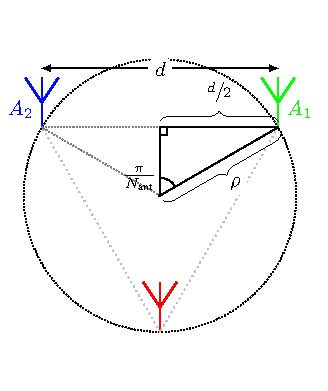
\includegraphics[scale=0.8]{../pictures/antennas_3.pdf}%
        % }
        % \vfill
    \end{frame}
    \begin{frame}{Cinco antenas}
        \centering%
        % \fbox{%
            % \scalebox{0.75}%
            % \resizebox{0.5\textwidth}{!}
            % {% \resizebox{!}{0.7\textheight}{%
\begin{circuitikz}[american, voltage shift=0.5, line width=0.5,every node/.style={font = {\footnotesize\bfseries}}]

    \def\wavelength{8}
    \pgfmathsetmacro\d{0.5*\wavelength}

    \def\signalAngle{75}
    \def\antennaAngle{120}

    \def\closeRange{9}
    \def\farRange{\closeRange+13}

	\def\NAntennas{5}
	\pgfmathsetmacro\AngleAntennas{360/\NAntennas}
	\pgfmathsetmacro\ShiftAngleAntennas{-90+\AngleAntennas}

	\pgfmathsetmacro\RhoAntennas{\d/(2*sin(180/\NAntennas))}

    \def\centerarc(#1)(#2:#3:#4)% Syntax: [draw options] (center) (initial angle:final angle:radius)
    { ($(#1)+({#4*cos(#2)},{#4*sin(#2)})$) arc (#2:#3:#4) }

    \def\coordref[#1](#2){%

        \coordinate(sysref) at (#2);

        \draw[#1, -latex] (sysref) ++(-0.4,-0.3) -- ++(0.9,0) node[midway, below]{$x$};
        \draw[#1, -latex] (sysref) ++(-0.3,-0.4) -- ++(0,0.9) node[midway, left]{$y$};
        \draw[#1, -latex] \centerarc(sysref)(-90:180:0.25);
        \draw[#1] (sysref) node{$+$}
    }

    \coordinate (bottomleft) at (-4,-4);
    \coordinate (topright) at (4,4);


    % \draw[Red,dashed] (bottomleft) rectangle (topright);
    \clip (bottomleft) rectangle (topright);

    \coordinate (O) at (0,0);
    \coordinate (sourceAntenna) at (\signalAngle:\closeRange*\wavelength);
    % \draw [help lines, dashed] (bottomleft) grid (topright); % desenha grid
    % \draw [red] (O) node[draw,cross out] {}; % marca pont(0,0)

	\draw[densely dotted] (O) circle (\RhoAntennas);

    \draw[thick, cmyk_G] (O) ++(1*\AngleAntennas+\ShiftAngleAntennas:\RhoAntennas) node[dinantenna] (A1) {} node [above right] {$A_{1}$};
    \draw[thick, cmyk_B] (O) ++(2*\AngleAntennas+\ShiftAngleAntennas:\RhoAntennas) node[dinantenna] (A2) {} node [above left] {$A_{2}$};
    \draw[thick, cmyk_R] (O) ++(3*\AngleAntennas+\ShiftAngleAntennas:\RhoAntennas) node[dinantenna] (A3) {};
    \draw[thick, cmyk_C] (O) ++(4*\AngleAntennas+\ShiftAngleAntennas:\RhoAntennas) node[dinantenna] (A4) {};
    \draw[thick, cmyk_M] (O) ++(5*\AngleAntennas+\ShiftAngleAntennas:\RhoAntennas) node[dinantenna] (A5) {};

	\coordinate (A1_2) at ($(A1)!0.5!(A2)$);

	\draw[Black!25, dotted]
		(A1) --
		(A5) --
		(A4) --
		(A3) --
		(A2)
	;

	\draw[Black!50, densely dotted]
		(O) --
		(A2) --
		(A1_2)
	;

	\draw
		(A1) --
		(O) --
		(A1_2) --
		(A1)
	;

	\draw
         (A1_2)
           ++(0:0.125)
         --++(-90:0.125)
         --++(+180:0.125)
	;

	\node at (O) {\tiny\textbullet};

	\draw
		(O) ++(90:0.3) node[left, inner sep=1.5pt] {$\textstyle \frac{\pi}{N_\text{ant}}$}
		\centerarc(O)(1*\AngleAntennas+\ShiftAngleAntennas:90:0.3)
	;


    % Distânci d entre antenas
    \draw[latex-latex]
        ($(A1)+(0,1)$) -- ($(A2)+(0,1)$) node [midway, fill=white, circle, inner sep=1pt] {$d$}
    ;

    \draw[decorate, decoration={brace, amplitude=5pt}, thin]
    ($(A1)+({1*\AngleAntennas+\ShiftAngleAntennas-90}:0.1)$)
    -- coordinate (brace)
    ($(O)+({1*\AngleAntennas+\ShiftAngleAntennas-90}:0.1)$)
    ;

    \draw (brace) ++({1*\AngleAntennas+\ShiftAngleAntennas-90}:5pt)
        node[anchor=north west, circle, fill=white, inner sep=1pt] {$\rho$}
    ;

	\draw[decorate, decoration={brace, amplitude=5pt}, thin]
    ($(A1_2)+({90}:0.1)$)
    -- coordinate (brace)
    ($(A1)+({90}:0.1)$)
    ;

    \draw (brace) ++({90}:5pt)
        node[anchor=south, circle, inner sep=1pt] {$\sfrac{d}{2}$}
    ;

    % \coordref[Black!25](3.5,0);

\end{circuitikz}
% }

}%
            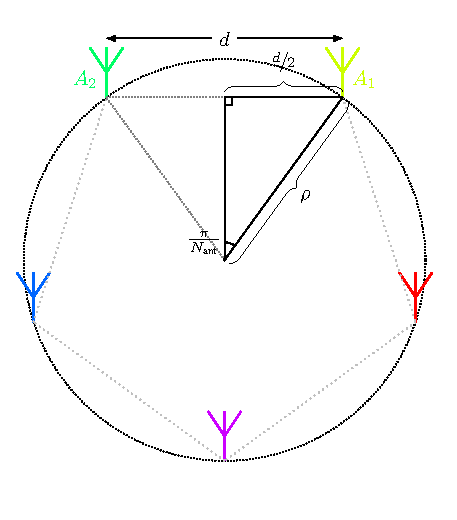
\includegraphics[scale=0.8]{../pictures/antennas_5.pdf}%
        % }
        % \vfill
    \end{frame}
    \begin{frame}{Sete antenas}
        \centering%
        % \fbox{%
            % \scalebox{0.75}%
            % \resizebox{0.5\textwidth}{!}
            % {% \resizebox{!}{0.7\textheight}{%
\begin{circuitikz}[american, voltage shift=0.5, line width=0.5,every node/.style={font = {\footnotesize\bfseries}}]

    \def\wavelength{8}
    \pgfmathsetmacro\d{0.5*\wavelength}

    \def\signalAngle{75}
    \def\antennaAngle{120}

    \def\closeRange{9}
    \def\farRange{\closeRange+13}

	\def\NAntennas{7}
	\pgfmathsetmacro\AngleAntennas{360/\NAntennas}
	\pgfmathsetmacro\ShiftAngleAntennas{-90+2*\AngleAntennas}

	\pgfmathsetmacro\RhoAntennas{\d/(2*sin(180/\NAntennas))}

    \def\centerarc(#1)(#2:#3:#4)% Syntax: [draw options] (center) (initial angle:final angle:radius)
    { ($(#1)+({#4*cos(#2)},{#4*sin(#2)})$) arc (#2:#3:#4) }

    \def\coordref[#1](#2){%

        \coordinate(sysref) at (#2);

        \draw[#1, -latex] (sysref) ++(-0.4,-0.3) -- ++(0.9,0) node[midway, below]{$x$};
        \draw[#1, -latex] (sysref) ++(-0.3,-0.4) -- ++(0,0.9) node[midway, left]{$y$};
        \draw[#1, -latex] \centerarc(sysref)(-90:180:0.25);
        \draw[#1] (sysref) node{$+$}
    }

    \pgfmathsetmacro\vSize{\RhoAntennas + 1}
    \pgfmathsetmacro\hSize{\RhoAntennas + 0.4}

    \coordinate (bottomleft) at (-\hSize,-\vSize);
    \coordinate (topright) at (\hSize,\vSize);

    % \draw[Red, thick]
    %     (bottomleft) -- (topright)
    %     (\hSize,-\vSize) -- (-\hSize,\vSize)
    % ;

    % \draw[Red,dashed] (bottomleft) rectangle (topright);
    \clip (bottomleft) rectangle (topright);

    \coordinate (O) at (0,0);
    \coordinate (sourceAntenna) at (\signalAngle:\closeRange*\wavelength);
    % \draw [help lines, dashed] (bottomleft) grid (topright); % desenha grid
    % \draw [red] (O) node[draw,cross out] {}; % marca pont(0,0)

	\draw[densely dotted] (O) circle (\RhoAntennas);

    \draw[thick, antena_7_1] (O) ++(1*\AngleAntennas+\ShiftAngleAntennas:\RhoAntennas) node[dinantenna] (A1) {} node [above right] {$A_{1}$};
    \draw[thick, antena_7_2] (O) ++(2*\AngleAntennas+\ShiftAngleAntennas:\RhoAntennas) node[dinantenna] (A2) {} node [above left] {$A_{2}$};
    \draw[thick, antena_7_3] (O) ++(3*\AngleAntennas+\ShiftAngleAntennas:\RhoAntennas) node[dinantenna] (A3) {};
    \draw[thick, antena_7_4] (O) ++(4*\AngleAntennas+\ShiftAngleAntennas:\RhoAntennas) node[dinantenna] (A4) {};
    \draw[thick, antena_7_5] (O) ++(5*\AngleAntennas+\ShiftAngleAntennas:\RhoAntennas) node[dinantenna] (A5) {};
    \draw[thick, antena_7_6] (O) ++(6*\AngleAntennas+\ShiftAngleAntennas:\RhoAntennas) node[dinantenna] (A6) {};
    \draw[thick, antena_7_7] (O) ++(7*\AngleAntennas+\ShiftAngleAntennas:\RhoAntennas) node[dinantenna] (A7) {};

	\coordinate (A1_2) at ($(A1)!0.5!(A2)$);

	\draw[Black!25, dotted]
		(A1) --
		(A7) --
		(A6) --
		(A5) --
		(A4) --
		(A3) --
		(A2)
	;

	\draw[Black!50, densely dotted]
		(O) --
		(A2) --
		(A1_2)
	;

	\draw
		(A1) --
		(O) --
		(A1_2) --
		(A1)
	;

	\draw
         (A1_2)
           ++(0:0.125)
         --++(-90:0.125)
         --++(+180:0.125)
	;

	\node at (O) {\tiny\textbullet};

	\draw
		(O) ++(90:0.3) node[left, inner sep=1.5pt] {$\textstyle \frac{\pi}{N_\text{ant}}$}
		\centerarc(O)(1*\AngleAntennas+\ShiftAngleAntennas:90:0.3)
	;


    % Distânci d entre antenas
    \draw[latex-latex]
        ($(A1)+(0,1)$) -- ($(A2)+(0,1)$) node [midway, fill=white, circle, inner sep=1pt] {$d$}
    ;

    \draw[decorate, decoration={brace, amplitude=5pt}, thin]
    ($(A1)+({1*\AngleAntennas+\ShiftAngleAntennas-90}:0.1)$)
    -- coordinate (brace)
    ($(O)+({1*\AngleAntennas+\ShiftAngleAntennas-90}:0.1)$)
    ;

    \draw (brace) ++({1*\AngleAntennas+\ShiftAngleAntennas-90}:5pt)
        node[anchor=north west, circle, fill=white, inner sep=1pt] {$\rho$}
    ;

	\draw[decorate, decoration={brace, amplitude=5pt}, thin]
    ($(A1_2)+({90}:0.1)$)
    -- coordinate (brace)
    ($(A1)+({90}:0.1)$)
    ;

    \draw (brace) ++({90}:5pt)
        node[anchor=south, circle, inner sep=1pt] {$\sfrac{d}{2}$}
    ;

    % \coordref[Black!25](3.5,0);

\end{circuitikz}
% }

}%
            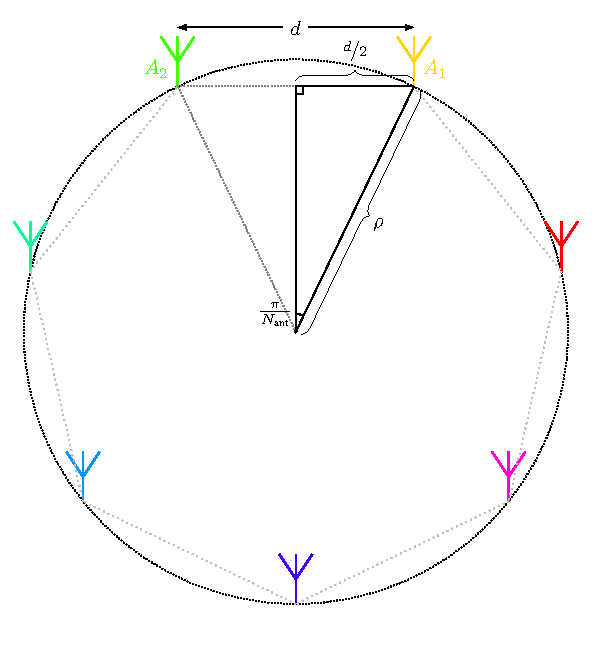
\includegraphics[scale=0.8]{../pictures/antennas_7.pdf}%
        % }
        % \vfill
    \end{frame}

\section{Calculo de fase}
    \begin{frame}{Geometria do sistema}
        \begin{equation*}
            T = \frac{2\pi}{\omega} = \frac{1}{f}
        \end{equation*}

        \begin{equation*}
            I_k =
            \int\limits_0^{T} \cos\left(\omega \cdot\tau\right)
            \cdot w\left( x_{A_k}, ~y_{A_k}, ~\tau \right) \partial \tau
        \end{equation*}

        \begin{equation*}
            Q_k =
            \int\limits_0^{T} \sin\left(\omega\cdot\tau\right)
            \cdot w\left( x_{A_k}, ~y_{A_k}, ~\tau \right) \partial \tau
        \end{equation*}

        \begin{equation*}
            \textcolor{cmyk_B}{Z_k} =
            \frac{\omega}{\pi}\cdot\left(I_k + \imath Q_k\right)
        \end{equation*}

        \begin{equation*}
            \Delta_\Phi =
            \textcolor{cmyk_B}{\Phi_k} - \textcolor{cmyk_R}{\Phi_{k+1}} =
            \arg\left(\textcolor{cmyk_B}{Z_k}\right) - \arg\left(\textcolor{cmyk_R}{Z_{k+1}}\right) =
            \arg\left(\textcolor{cmyk_B}{Z_k} \cdot \overline{\textcolor{cmyk_R}{Z_{k+1}}}\right)
        \end{equation*}

        \begin{equation*}
            \textcolor{Purple}{\beta_{\pm k}} = \arccos\left(\frac{\cancel{\lambda}}{\cancel{d}}\cdot\frac{\Delta_\Phi}{\cancel{2}\pi}\right)
        \end{equation*}

    \end{frame}

    \begin{frame}{Geometria do sistema}
        \centering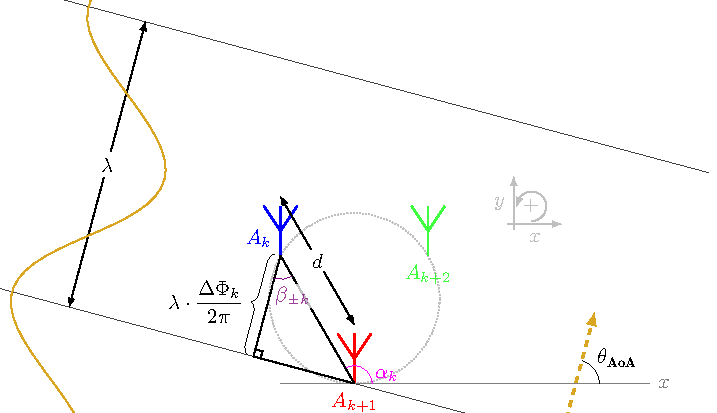
\includegraphics{../pictures/AoA_geometria.pdf}
    \end{frame}

    \begin{frame}{Determinar AoA}
        \begin{equation*}
            \theta_{\pm k} = \textcolor{cmyk_M}{\alpha_k}\pm \textcolor{Purple}{\beta_{\pm k}}
        \end{equation*}

        \begin{equation*}
            \Theta = \left\{\theta_{\pm k} ~\middle\vert~ \forall k\right\}
        \end{equation*}

        \begin{equation*}
            \delta = \frac{\pi}{2 \cdot \left( 1 + N_\text{ant} \right)}
        \end{equation*}

        \begin{equation*}
            \Theta_{\left\lfloor\bullet\right\rceil} =
            \left\{\left\lfloor\frac{\theta}{\delta}\right\rceil\cdot\delta ~\middle\vert~ \forall \theta \in \Theta  \right\}
        \end{equation*}

        \begin{equation*}
            \theta_\mathcal{M_o} = \operatorname{\mathcal{M_o}}\left( \Theta_{\left\lfloor\bullet\right\rceil}  \right)
        \end{equation*}

        \begin{equation*}
            \Theta_\text{F} = \left\{\theta \in \Theta  ~\middle\vert~
            \theta_\mathcal{M_o} - \delta \leq \theta \leq \theta_\mathcal{M_o} + \delta\right\}
        \end{equation*}

        \begin{equation*}
            \theta_\text{AoA} = \widetilde{\Theta_\text{F}}
        \end{equation*}
    \end{frame}

\section{Simulação}
    \begin{frame}{Definição de onda}
        % \begin{multicols}{2}
            \begin{equation*}
                r_0 = r \cdot \lambda
            \end{equation*}

            \begin{equation*}
                x_0 = r_0 \cdot \cos(\theta)
            \end{equation*}

            \begin{equation*}
                y_0 = r_0 \cdot \sin(\theta)
            \end{equation*}

            \begin{equation*}
                \mathcal{aux}_{\text{\lstinline|argument_r|}}(x, y, t, \theta, r, \phi, \lambda, \omega) =
                \frac{2\pi}{\lambda} \cdot \sqrt{(y - y_0)^2+(x - x_0)^2} + \omega \cdot t + \phi
            \end{equation*}

            \begin{equation*}
                w(x, y, t, \theta, r, \phi, \lambda, \omega) = \frac{\sin\left(\mathcal{aux}\right)+ \cos\left(\mathcal{aux}\right)}{\sqrt{2}}
            \end{equation*}
        % \end{multicols}
    \end{frame}


    \begin{frame}

        \centering
        \href{https://github.com/HeckRodSav/TG/blob/main/documentation/pictures/POLY_3/simul_POLY_3_R_50.gif}{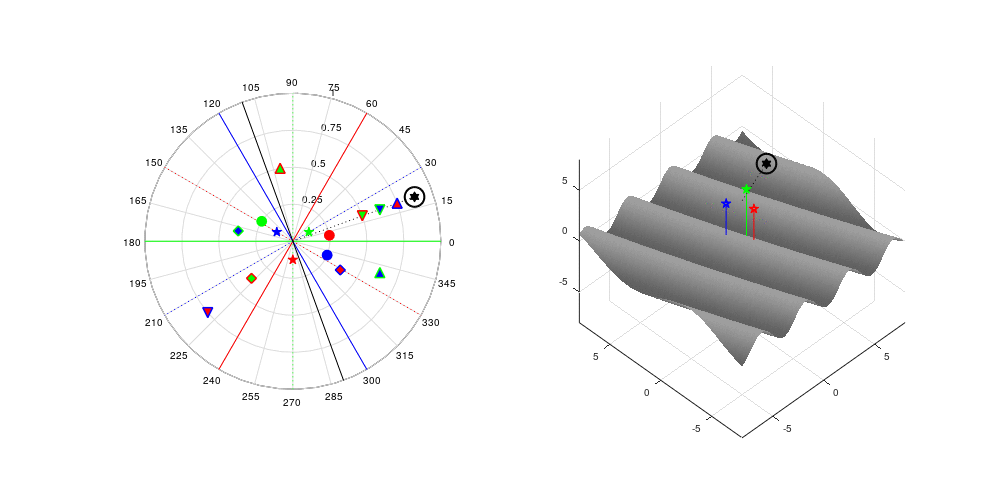
\includegraphics[width=\textwidth]{../pictures/simul_POLY_3_R_50.png}}

    \end{frame}

    % \begin{frame}{\href{https://drive.google.com/file/d/1-ep5hH8TSrnHU_m9b4AFmUJlB_hGR41m/view?usp=drive_link}{Análise de vetores complexos}}
    %     % \begin{multicols}{2}
    %         \begin{equation*}
    %             C(x,y) = \int_0^T w(x,y,t) \cdot \cos(k(x,y,t)) \partial t
    %         \end{equation*}

    %         \begin{equation*}
    %             S(x,y) = \int_0^T w(x,y,t) \cdot \sin(k(x,y,t)) \partial t
    %         \end{equation*}

    %         \begin{equation*}
    %             Z(x,y) = 2\cdot(S + \imath C)
    %         \end{equation*}

    %         \begin{equation*}
    %             \Delta_{x,y} = \arg(\textcolor{Green}{Z_{0,0}}\cdot Z^*_{x,y})
    %         \end{equation*}

    %         \begin{equation*}
    %             \text{componente}_{x,y} = -\frac{\Delta_{x,y}}{\pi}\cdot\frac{\cancel{\lambda}}{\cancel{d \cdot 2}} = -\frac{\Delta_{x,y}}{\pi}
    %         \end{equation*}
    %         % \end{multicols}
    % \end{frame}
    \section{Resultados}


\subsection{Simulação}

    \begin{frame}

        \centering
        \href{https://github.com/HeckRodSav/TG/blob/main/documentation/pictures/POLY_3/simul_POLY_3_R_50.gif}{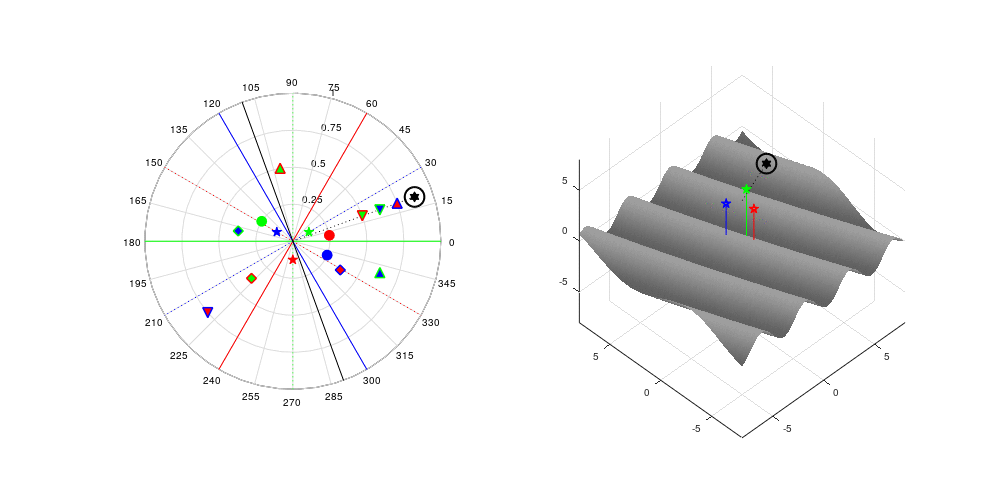
\includegraphics[width=\textwidth]{../pictures/simul_POLY_3_R_50.png}}

    \end{frame}

\subsection{Três antenas}
	\begin{frame}{R\textsuperscript{2} para três antenas}
		\begin{table}
			\centering
			\begin{tabular}{@{}
				S[table-format = 3.1]
				S[table-format = 3.2, table-model-setup = \bfseries]
				S[table-format = 3.2, table-model-setup = \bfseries]
				@{}}
				\toprule
				{SNR (\unit{\deci\bel})} & {R\textsuperscript{2} sem ATT (\unit{\percent})} & {R\textsuperscript{2} com ATT (\unit{\percent})}
				\\\midrule
				\infinity & \bfseries 100.00 & 100.00\\
				20 & 88.06 & 90.45\\
				17 & 88.18 & 87.98\\
				14 & 99.99 & 84.49\\
				7 & 90.12 & 83.50\\
				0 & \bfseries 76.32 & \bfseries 78.73\\
				\bottomrule
			\end{tabular}
			\caption*{\tiny Fonte: Autor, saídas das simulações disponíveis em \href{https://github.com/HeckRodSav/TG/tree/main/documentation/data/POLY_3}{\underline{GitHub}}.}
		\end{table}
	\end{frame}

	\begin{frame}
		\begin{figure}
			\centering
			\caption*{Caso ideal ($\text{SNR} \rightarrow \qty{\infinity}{\deci\bel}$).}
			% \begin{tikzpicture}
    % \pgfsetfillopacity{0.5}

    \def\fileName{simul_POLY_3_R_50}
    \def\fileAddress{../../code/simul/Output/POLY_3/\fileName.dat}
    % \def\fileAddress{../data/\fileName.dat}

    \def\height{.225\linewidth}
    \def\width{0.75\linewidth}
    \def\distance{0.25cm}
    \def\xmin{-1}
    \def\xmax{101}

    \begin{axis} %configuração do eixo Y esquerdo e eixo X
    [
        name=plot1,
        reverse legend, % inverte a ordem que os items aparecem na legenda
    	% legend style={
        % 	at=(current bounding box.north),
        % 	anchor=south,
        % 	legend columns=6,
        % 	transpose legend,
        % 	draw=none,
        % 	/tikz/every even column/.append style={column sep=0.5cm}
    	% }, % onde exibir
        % axis x line=center,
        % axis y line=center,
        height=\height, % altura da região do gráfico
        width=\width, % largura da região do gráfico
        scale only axis, %
        minor grid style={densely dotted}, % estilo da grade secundária
        major grid style={densely dashed}, % estilo da grade principal
        grid style={lightgray, thin}, % cor das grades
        % axis on top, % forçar grade para ficar por cima do gráfico
        %
        %
        % axis y line*=left, % define gráfico para usar eixo esquerdo sem exibir direito
        y tick label style={
            /pgf/number format/.cd,
            fixed,
            % fixed zerofill,
            precision=1, % quantidade de casas depois da virgula
            /tikz/.cd
        },
        % y filter/.expression={y==0 ? NaN : y},
        scaled y ticks = false,
        ylabel={$\alpha_{k}\pm \beta_{k}$ (\si{\radian})}, % titulo eixo vertical
        % yticklabel={\pgfmathparse{\tick-50}\pgfmathprintnumber{\pgfmathresult}}, % fator multiplicativo para valores do eixo
        y tick label style={/pgf/number format/1000 sep=}, % Altera marcação de milhar
        % yticklabel style={rotate=90},
		ytick={-3.1415, -1.5708, 0, 1.5708, 3.1415},
		yticklabels={$-\pi$,$-\dfrac{\pi}{2}$,$0$,$\dfrac{\pi}{2}$,$\pi$},
        % ytick={0,1,2,3,4,5}, % lista de valores a serem utilizados no eixo
        % ymin=-1,  ymax=4,  % intervalo de valores no eixo y -> na dúvida, deixe comentado
        %
        ymajorgrids=true, % exibir grade principal y
        yminorgrids=true, % exibir grade secundária y
        minor y tick num=4, % contagem de linhas na grade secundária y
        % ybar,
        %
        %
        xlabel={$\theta_{DoA}$ (\si{\radian})}, % título eixo horizontal
        % xticklabel={\pgfmathparse{\tick-50}\pgfmathprintnumber{\pgfmathresult}}, % fator multiplicativo para valores do eixo
        % xticklabels={}, % fator multiplicativo para valores do eixo
		% xtick={0, 12.5, 25, 37.5, 50, 62.6, 75, 87.5, 100},
		% xticklabels={$-2~\pi$,$-\dfrac{3~\pi}{2}$,$-\pi$,$-\dfrac{\pi}{2}$,$0$,$-\dfrac{\pi}{2}$,$\pi$,$-\dfrac{3~\pi}{2}$,$2~\pi$},
		xtick={0, 25, 50, 75, 100},
		xticklabels={$-2 \pi$,$-\pi$,$0$,$\pi$,$2 \pi$},
        % xmode=log,
        % log ticks with fixed point,
        % x filter/.code=\pgfmathparse{#1 + 6.90775527898214},
        x tick label style={
            /pgf/number format/.cd,
            fixed,
            % fixed zerofill,
            precision=1,
            /tikz/.cd,
            /pgf/number format/use comma
        },
        xmin=\xmin, xmax=\xmax, % intervalo de valores no eixo x -> na dúvida, deixe comentado
        scaled x ticks = false,
        %
        xmajorgrids=true, % exibir grade principal x
        xminorgrids=true, % exibir grade secundária x
        minor x tick num=7, % contagem de linhas na grade secundária x
        %
        %
        %
        % unbounded coords=jump,
        % jump threshold/.initial=0.25
    ]

	\addplot[
        cmyk_G,
        mark=triangle*,
		opacity=0.5,
        only marks,
        % smooth
    ] table [
        % col sep=comma,
        x=percent, % cabeçalho da coluna de dados X no arquivo
        y=delta_1_x_3, % cabeçalho da coluna de dados Y no arquivo
    ]
    {\fileAddress};	\label{\fileName.1.1}

    \addplot[
        cmyk_G,
        mark=triangle*,
		opacity=0.5,
		mark options={rotate=180},
        only marks,
        % smooth
    ] table [
        % col sep=comma,
        x=percent, % cabeçalho da coluna de dados X no arquivo
        y=delta_3_x_1, % cabeçalho da coluna de dados Y no arquivo
    ]
    {\fileAddress};	\label{\fileName.1.2}

	\addplot[
        cmyk_B,
        mark=triangle*,
		opacity=0.5,
        only marks,
        % smooth
    ] table [
        % col sep=comma,
        x=percent, % cabeçalho da coluna de dados X no arquivo
        y=delta_2_x_1, % cabeçalho da coluna de dados Y no arquivo
    ]
    {\fileAddress};	\label{\fileName.1.3}

    \addplot[
        cmyk_B,
        mark=triangle*,
		opacity=0.5,
		mark options={rotate=180},
        only marks,
        % smooth
    ] table [
        % col sep=comma,
        x=percent, % cabeçalho da coluna de dados X no arquivo
        y=delta_1_x_2, % cabeçalho da coluna de dados Y no arquivo
    ]
    {\fileAddress};	\label{\fileName.1.4}

	\addplot[
        cmyk_R,
        mark=triangle*,
		opacity=0.5,
        only marks,
        % smooth
    ] table [
        % col sep=comma,
        x=percent, % cabeçalho da coluna de dados X no arquivo
        y=delta_3_x_2, % cabeçalho da coluna de dados Y no arquivo
    ]
    {\fileAddress};	\label{\fileName.1.5}

    \addplot[
        cmyk_R,
        mark=triangle*,
		opacity=0.5,
		mark options={rotate=180},
        only marks,
        % smooth
    ] table [
        % col sep=comma,
        x=percent, % cabeçalho da coluna de dados X no arquivo
        y=delta_2_x_3, % cabeçalho da coluna de dados Y no arquivo
    ]
    {\fileAddress};	\label{\fileName.1.6}

    \end{axis}

    % \begin{axis} %configuração do eixo Y direito e legenda
    % [
    %     legend cell align=left, % alinhamento de texto na legenda
    %     % legend pos={outer north east}, % onde exibir caixa de legenda
    %     % reverse legend, % inverte a ordem que os items aparecem na legenda
    % 	legend style={
    %     	at=(current bounding box.north),
    %     	anchor=south,
    %     	legend columns=2,
    %     % 	transpose legend,
    %     	draw=none
    % 	}, % onde exibir
    %     % axis x line=center,
    %     % axis y line=center,
    %     height=\height, % altura da região do gráfico
    %     width=\width, % largura da região do gráfico
    %     scale only axis, %
    %     minor grid style={densely dotted}, % estilo da grade secundária
    %     major grid style={densely dashed}, % estilo da grade principal
    %     grid style={lightgray, thin}, % cor das grades
    %     % axis on top, % forçar grade para ficar por cima do gráfico
    %     %
    %     %
    %     axis y line*=right, % define gráfico para usar eixo direito sem exibir esquerdo
    %     ylabel={$V_{out}$ (\si{\milli\volt})}, % titulo eixo vertical
    %     y tick label style={
    %         /pgf/number format/.cd,
    %         fixed,
    %         % fixed zerofill,
    %         precision=3, % quantidade de casas depois da virgula
    %         /tikz/.cd,
    %         /pgf/number format/use comma
    %     },
    %     % y filter/.expression={y==0 ? NaN : y},
    %     scaled y ticks = false,
    %     % yticklabel={\pgfmathparse{\tick*10^3}\pgfmathprintnumber{\pgfmathresult}}, % fator multiplicativo para valores do eixo
    %     y tick label style={/pgf/number format/1000 sep=}, % Altera marcação de milhar
    %     % yticklabel style={rotate=90},
    %     % ytick={-12,-6,0,6,12}, % lista de valores a serem utilizados no eixo
    %     % ymin=0.76503, ymax=0.76509,  % intervalo de valores no eixo y -> na dúvida, deixe comentado
    %     %
    %     ymajorgrids=false, % exibir grade principal y
    %     yminorgrids=false, % exibir grade secundária y
    %     minor y tick num=4, % contagem de linhas na grade secundária y
    %     % ybar,
    %     %
    %     %
    %     axis x line=none, %oculta eixo inferior quando o gráfico anterior já exibe
    %     % xlabel={Frequência (\si{\hertz})}, % título eixo horizontal
    %     % xticklabel={\pgfmathparse{\tick*10^3}\pgfmathprintnumber{\pgfmathresult}}, % fator multiplicativo para valores do eixo
    %     % xmode=log,
    %     % log ticks with fixed point,
    %     % x filter/.code=\pgfmathparse{#1 + 6.90775527898214},
    %     % x tick label style={
    %     %     /pgf/number format/.cd,
    %     %     fixed,
    %     %     % fixed zerofill,
    %     %     precision=0,
    %     %     /tikz/.cd,
    %     %     /pgf/number format/use comma
    %     % },
    %     xmin=\xmin, xmax=\xmax, % intervalo de valores no eixo x -> na dúvida, deixe comentado
    %     % scaled x ticks = true,
    %     %
    %     % xmajorgrids=true, % exibir grade principal x
    %     % xminorgrids=true, % exibir grade secundária x
    %     % minor x tick num=7, % contagem de linhas na grade secundária x
    %     %
    %     %
    %     %
    % ]



    % \addplot[mark=none,red, thick]
    % table [
    %     x=time, % cabeçalho da coluna de dados X no arquivo
    %     y=vout % cabeçalho da coluna de dados Y no arquivo
    % ]
    % {graficos/dados/booster.dat};  \label{\fileName.1.2}

    % % \addlegendimage{/pgfplots/refstyle=_1_2}

    % % \addplot[ForestGreen, densely dashdotted, thick]
    % % coordinates
    % % {
    % %     (\pgfkeysvalueof{/pgfplots/xmin},12)
    % %     (\pgfkeysvalueof{/pgfplots/xmax},12)
    % % };
    % % % \addlegendentry{$V_{out}=\pm\SI{12}{\volt}$}

    % % \addplot[ForestGreen, densely dashdotted, thick]
    % % coordinates
    % % {
    % %     (\pgfkeysvalueof{/pgfplots/xmin},-12)
    % %     (\pgfkeysvalueof{/pgfplots/xmax},-12)
    % % };

    % \end{axis}

    \begin{axis} %configuração do eixo Y esquerdo e eixo X
    [
        at={($(plot1.north)+(0,\distance)$)},
        anchor=south,
        % reverse legend, % inverte a ordem que os items aparecem na legenda
		legend style={
        	at=(current bounding box.north),
        	anchor=south,
        	legend columns=2,
        	transpose legend,
        	draw=none,
        	/tikz/every even column/.append style={column sep=0.5cm}
    	}, % onde exibir
        samples=505,
        domain=0:100,
        % axis x line=center,
        % axis y line=center,
        height=\height, % altura da região do gráfico
        width=\width, % largura da região do gráfico
        scale only axis, %
        minor grid style={densely dotted}, % estilo da grade secundária
        major grid style={densely dashed}, % estilo da grade principal
        grid style={lightgray, thin}, % cor das grades
        % axis on top, % forçar grade para ficar por cima do gráfico
        %
        %
        % axis y line*=left, % define gráfico para usar eixo esquerdo sem exibir direito
        y tick label style={
            /pgf/number format/.cd,
            fixed,
            % fixed zerofill,
            precision=1, % quantidade de casas depois da virgula
            /tikz/.cd
        },
        % y filter/.expression={y==0 ? NaN : y},
        scaled y ticks = false,
        ylabel={$\theta$ (\si{\radian})}, % titulo eixo vertical
        % yticklabel={\pgfmathparse{\tick*10^3}\pgfmathprintnumber{\pgfmathresult}}, % fator multiplicativo para valores do eixo
        y tick label style={/pgf/number format/1000 sep=}, % Altera marcação de milhar
        % yticklabel style={rotate=90},
		ytick={-3.1415, -1.5708, 0, 1.5708, 3.1415},
		yticklabels={$-\pi$,$-\dfrac{\pi}{2}$,$0$,$\dfrac{\pi}{2}$,$\pi$},
        % ytick={0,1,2,3,4,5}, % lista de valores a serem utilizados no eixo
        % ymin=-1,  ymax=4,  % intervalo de valores no eixo y -> na dúvida, deixe comentado
        %
        ymajorgrids=true, % exibir grade principal y
        yminorgrids=true, % exibir grade secundária y
        minor y tick num=4, % contagem de linhas na grade secundária y
        % ybar,
        %
        %
        % xlabel={Tempo (\si{\milli\second})}, % título eixo horizontal
        % xticklabel={\pgfmathparse{\tick*10^3}\pgfmathprintnumber{\pgfmathresult}}, % fator multiplicativo para valores do eixo
		xtick={0, 25, 50, 75, 100},
        xticklabels={}, % fator multiplicativo para valores do eixo
        % xmode=log,
        % log ticks with fixed point,
        % x filter/.code=\pgfmathparse{#1 + 6.90775527898214},
        x tick label style={
            /pgf/number format/.cd,
            fixed,
            % fixed zerofill,
            precision=1,
            /tikz/.cd,
            /pgf/number format/use comma
        },
        xmin=\xmin, xmax=\xmax, % intervalo de valores no eixo x -> na dúvida, deixe comentado
        scaled x ticks = false,
        %
        xmajorgrids=true, % exibir grade principal x
        xminorgrids=true, % exibir grade secundária x
        minor x tick num=7, % contagem de linhas na grade secundária x
        %
        %
        %
        unbounded coords=jump,
		jump threshold/.initial=0.01
    ]


    \addplot[
        Black,
        mark=*,
		mark size=0.5pt,
        only marks,
        % smooth
    ] table [
        % col sep=comma,
        x=percent, % cabeçalho da coluna de dados X no arquivo
        y=choose_angle, % cabeçalho da coluna de dados Y no arquivo
	]
	{\fileAddress};	\addlegendentry{$\theta_{AoA}$}

	% \addplot[
	% 	Black,
	% 	mark=o,
	% 	mark size=1.5pt,
	% 	only marks,
	% 	opacity=0.5,
    %     thick,
	% 	% smooth
	% ] table [
	% 	% col sep=comma,
	% 	x=percent, % cabeçalho da coluna de dados X no arquivo
	% 	y=ang_W, % cabeçalho da coluna de dados Y no arquivo
	% ]
	% {\fileAddress};
    \addplot [
        Black,
        opacity=0.5,
        mark=none,
        mark size=5pt,
        very thick,
        % only marks,
        % smooth
    ] {((x==25)||(x==75)?nan:pi*(mod(x+25,50)-25)/25)};
    \addlegendentry{$\theta_{DoA}$}


	\addlegendimage{/pgfplots/refstyle=\fileName.1.1}\addlegendentry{$\theta_{+1}$}
	\addlegendimage{/pgfplots/refstyle=\fileName.1.2}\addlegendentry{$\theta_{-1}$}

	\addlegendimage{/pgfplots/refstyle=\fileName.1.3}\addlegendentry{$\theta_{+2}$}
	\addlegendimage{/pgfplots/refstyle=\fileName.1.4}\addlegendentry{$\theta_{-2}$}

    \addlegendimage{/pgfplots/refstyle=\fileName.1.5}\addlegendentry{$\theta_{+3}$}
	\addlegendimage{/pgfplots/refstyle=\fileName.1.6}\addlegendentry{$\theta_{-3}$}


    \end{axis}

    % \begin{axis} %configuração do eixo Y direito e legenda
    % [
    %     at={($(plot1.north)+(0,\distance)$)},
    %     anchor=south,
    %     legend cell align=left, % alinhamento de texto na legenda
    %     % legend pos={outer north east}, % onde exibir caixa de legenda
    %     % reverse legend, % inverte a ordem que os items aparecem na legenda
    % 	legend style={
    %     	at=(current bounding box.north),
    %     	anchor=south,
    %     	legend columns=3,
    %     % 	transpose legend,
    %     	draw=none,
    %     	/tikz/every even column/.append style={column sep=0.5cm}
    % 	}, % onde exibir
    %     % axis x line=center,
    %     % axis y line=center,
    %     height=\height, % altura da região do gráfico
    %     width=\width, % largura da região do gráfico
    %     scale only axis, %
    %     minor grid style={densely dotted}, % estilo da grade secundária
    %     major grid style={densely dashed}, % estilo da grade principal
    %     grid style={lightgray, thin}, % cor das grades
    %     % axis on top, % forçar grade para ficar por cima do gráfico
    %     %
    %     %
    %     axis y line*=right, % define gráfico para usar eixo direito sem exibir esquerdo
    %     ylabel={$V_{out}$ (\si{\volt})}, % titulo eixo vertical
    %     y tick label style={
    %         /pgf/number format/.cd,
    %         fixed,
    %         % fixed zerofill,
    %         precision=3, % quantidade de casas depois da virgula
    %         /tikz/.cd,
    %         /pgf/number format/use comma
    %     },
    %     % y filter/.expression={y==0 ? NaN : y},
    %     scaled y ticks = false,
    %     % yticklabel={\pgfmathparse{\tick*10^3}\pgfmathprintnumber{\pgfmathresult}}, % fator multiplicativo para valores do eixo
    %     y tick label style={/pgf/number format/1000 sep=}, % Altera marcação de milhar
    %     % yticklabel style={rotate=90},
    %     % ytick={-12,-6,0,6,12}, % lista de valores a serem utilizados no eixo
    %     % ymin=0.76503, ymax=0.76509,  % intervalo de valores no eixo y -> na dúvida, deixe comentado
    %     %
    %     ymajorgrids=false, % exibir grade principal y
    %     yminorgrids=false, % exibir grade secundária y
    %     minor y tick num=4, % contagem de linhas na grade secundária y
    %     % ybar,
    %     %
    %     %
    %     axis x line=none, %oculta eixo inferior quando o gráfico anterior já exibe
    %     % xlabel={Frequência (\si{\hertz})}, % título eixo horizontal
    %     % xticklabel={\pgfmathparse{\tick*10^3}\pgfmathprintnumber{\pgfmathresult}}, % fator multiplicativo para valores do eixo
    %     % xmode=log,
    %     % log ticks with fixed point,
    %     % x filter/.code=\pgfmathparse{#1 + 6.90775527898214},
    %     % x tick label style={
    %     %     /pgf/number format/.cd,
    %     %     fixed,
    %     %     % fixed zerofill,
    %     %     precision=0,
    %     %     /tikz/.cd,
    %     %     /pgf/number format/use comma
    %     % },
    %     xmin=\xmin, xmax=\xmax, % intervalo de valores no eixo x -> na dúvida, deixe comentado
    %     % scaled x ticks = true,
    %     %
    %     % xmajorgrids=true, % exibir grade principal x
    %     % xminorgrids=true, % exibir grade secundária x
    %     % minor x tick num=10, % contagem de linhas na grade secundária x
    %     %
    %     %
    %     %
    % ]


    % \addlegendimage{/pgfplots/refstyle=_2_1}\addlegendentry{$V_{in}$}
    % \addlegendimage{/pgfplots/refstyle=_2_2}\addlegendentry{$V_{in}$}
    % % \addplot[mark=none,red, thick]
    % % table [
    % %     x=time, % cabeçalho da coluna de dados X no arquivo
    % %     y=vout % cabeçalho da coluna de dados Y no arquivo
    % % ]
    % % {graficos/dados/booster.dat}; % \label{\fileName.1.2}
    % % \addlegendentry{$V_{out}$}

    % \addlegendimage{/pgfplots/refstyle=_1_1}\addlegendentry{$I_{out}$}
    % \addlegendimage{/pgfplots/refstyle=_1_2}\addlegendentry{$I_{out}$}

    % % \addlegendimage{/pgfplots/refstyle=_1_2}

    % % \addplot[ForestGreen, densely dashdotted, thick]
    % % coordinates
    % % {
    % %     (\pgfkeysvalueof{/pgfplots/xmin},12)
    % %     (\pgfkeysvalueof{/pgfplots/xmax},12)
    % % };
    % % % \addlegendentry{$V_{out}=\pm\SI{12}{\volt}$}

    % % \addplot[ForestGreen, densely dashdotted, thick]
    % % coordinates
    % % {
    % %     (\pgfkeysvalueof{/pgfplots/xmin},-12)
    % %     (\pgfkeysvalueof{/pgfplots/xmax},-12)
    % % };

    % \end{axis}



\end{tikzpicture}

			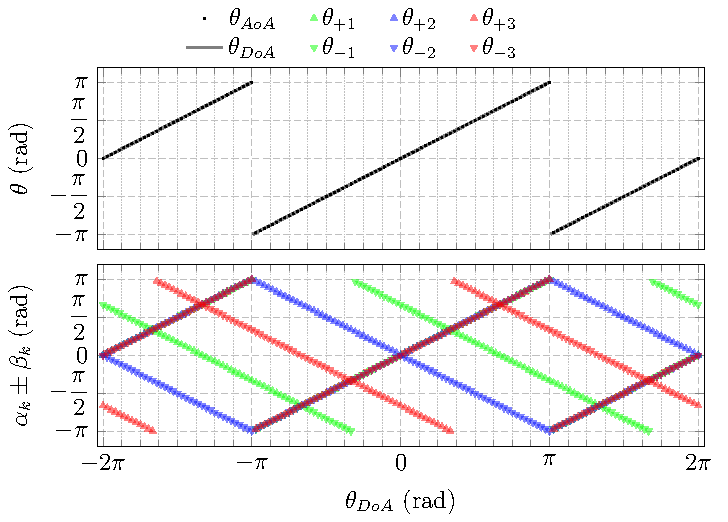
\includegraphics[height=0.785\textheight]{../pictures/simul_POLY_3_R_50.pdf}
			\caption*{\tiny Fonte: Autor, saída gráfica disponível em \href{https://github.com/HeckRodSav/TG/blob/main/documentation/pictures/POLY_3/simul_POLY_3_R_50.gif}{\underline{GitHub}}.}
		\end{figure}
	\end{frame}
	\begin{frame}
		\begin{figure}
			\centering
			\caption*{Caso $\text{SNR} = \SI{0}{\deci\bel}$, sem atenuação.}
			% \begin{tikzpicture}
    % \pgfsetfillopacity{0.5}

    \def\fileName{simul_POLY_3_R_50_SNR_1}
    \def\fileAddress{../../code/simul/Output/POLY_3/\fileName.dat}
	% \def\fileAddress{../data/\fileName.dat}

    \def\height{.25\linewidth}
    \def\width{0.75\linewidth}
    \def\distance{0.25cm}
    \def\xmin{-1}
    \def\xmax{101}

    \begin{axis} %configuração do eixo Y esquerdo e eixo X
    [
        name=plot1,
        reverse legend, % inverte a ordem que os items aparecem na legenda
    	% legend style={
        % 	at=(current bounding box.north),
        % 	anchor=south,
        % 	legend columns=6,
        % 	transpose legend,
        % 	draw=none,
        % 	/tikz/every even column/.append style={column sep=0.5cm}
    	% }, % onde exibir
        % axis x line=center,
        % axis y line=center,
        height=\height, % altura da região do gráfico
        width=\width, % largura da região do gráfico
        scale only axis, %
        minor grid style={densely dotted}, % estilo da grade secundária
        major grid style={densely dashed}, % estilo da grade principal
        grid style={lightgray, thin}, % cor das grades
        % axis on top, % forçar grade para ficar por cima do gráfico
        %
        %
        % axis y line*=left, % define gráfico para usar eixo esquerdo sem exibir direito
        y tick label style={
            /pgf/number format/.cd,
            fixed,
            % fixed zerofill,
            precision=1, % quantidade de casas depois da virgula
            /tikz/.cd
        },
        % y filter/.expression={y==0 ? NaN : y},
        scaled y ticks = false,
        ylabel={$\alpha_{k}\pm \beta_{k}$ (\si{\radian})}, % titulo eixo vertical
        % yticklabel={\pgfmathparse{\tick-50}\pgfmathprintnumber{\pgfmathresult}}, % fator multiplicativo para valores do eixo
        y tick label style={/pgf/number format/1000 sep=}, % Altera marcação de milhar
        % yticklabel style={rotate=90},
		ytick={-3.1415, -1.5708, 0, 1.5708, 3.1415},
		yticklabels={$-\pi$,$-\dfrac{\pi}{2}$,$0$,$\dfrac{\pi}{2}$,$\pi$},
        % ytick={0,1,2,3,4,5}, % lista de valores a serem utilizados no eixo
        % ymin=-1,  ymax=4,  % intervalo de valores no eixo y -> na dúvida, deixe comentado
        %
        ymajorgrids=true, % exibir grade principal y
        yminorgrids=true, % exibir grade secundária y
        minor y tick num=4, % contagem de linhas na grade secundária y
        % ybar,
        %
        %
        xlabel={$\theta_{DoA}$ (\si{\radian})}, % título eixo horizontal
        % xticklabel={\pgfmathparse{\tick-50}\pgfmathprintnumber{\pgfmathresult}}, % fator multiplicativo para valores do eixo
        % xticklabels={}, % fator multiplicativo para valores do eixo
		% xtick={0, 12.5, 25, 37.5, 50, 62.6, 75, 87.5, 100},
		% xticklabels={$-2~\pi$,$-\dfrac{3~\pi}{2}$,$-\pi$,$-\dfrac{\pi}{2}$,$0$,$-\dfrac{\pi}{2}$,$\pi$,$-\dfrac{3~\pi}{2}$,$2~\pi$},
		xtick={0, 25, 50, 75, 100},
		xticklabels={$-2 \pi$,$-\pi$,$0$,$\pi$,$2 \pi$},
        % xmode=log,
        % log ticks with fixed point,
        % x filter/.code=\pgfmathparse{#1 + 6.90775527898214},
        x tick label style={
            /pgf/number format/.cd,
            fixed,
            % fixed zerofill,
            precision=1,
            /tikz/.cd,
            /pgf/number format/use comma
        },
        xmin=\xmin, xmax=\xmax, % intervalo de valores no eixo x -> na dúvida, deixe comentado
        scaled x ticks = false,
        %
        xmajorgrids=true, % exibir grade principal x
        xminorgrids=true, % exibir grade secundária x
        minor x tick num=7, % contagem de linhas na grade secundária x
        %
        %
        %
        % unbounded coords=jump,
        % jump threshold/.initial=0.25
    ]

	\addplot[
        cmyk_G,
        mark=triangle*,
		opacity=0.5,
        only marks,
        % smooth
    ] table [
        % col sep=comma,
        x=percent, % cabeçalho da coluna de dados X no arquivo
        y=delta_1_x_3, % cabeçalho da coluna de dados Y no arquivo
    ]
    {\fileAddress};	\label{\fileName.1.1}

    \addplot[
        cmyk_G,
        mark=triangle*,
		opacity=0.5,
		mark options={rotate=180},
        only marks,
        % smooth
    ] table [
        % col sep=comma,
        x=percent, % cabeçalho da coluna de dados X no arquivo
        y=delta_3_x_1, % cabeçalho da coluna de dados Y no arquivo
    ]
    {\fileAddress};	\label{\fileName.1.2}

	\addplot[
        cmyk_B,
        mark=triangle*,
		opacity=0.5,
        only marks,
        % smooth
    ] table [
        % col sep=comma,
        x=percent, % cabeçalho da coluna de dados X no arquivo
        y=delta_2_x_1, % cabeçalho da coluna de dados Y no arquivo
    ]
    {\fileAddress};	\label{\fileName.1.3}

    \addplot[
        cmyk_B,
        mark=triangle*,
		opacity=0.5,
		mark options={rotate=180},
        only marks,
        % smooth
    ] table [
        % col sep=comma,
        x=percent, % cabeçalho da coluna de dados X no arquivo
        y=delta_1_x_2, % cabeçalho da coluna de dados Y no arquivo
    ]
    {\fileAddress};	\label{\fileName.1.4}

	\addplot[
        cmyk_R,
        mark=triangle*,
		opacity=0.5,
        only marks,
        % smooth
    ] table [
        % col sep=comma,
        x=percent, % cabeçalho da coluna de dados X no arquivo
        y=delta_3_x_2, % cabeçalho da coluna de dados Y no arquivo
    ]
    {\fileAddress};	\label{\fileName.1.5}

    \addplot[
        cmyk_R,
        mark=triangle*,
		opacity=0.5,
		mark options={rotate=180},
        only marks,
        % smooth
    ] table [
        % col sep=comma,
        x=percent, % cabeçalho da coluna de dados X no arquivo
        y=delta_2_x_3, % cabeçalho da coluna de dados Y no arquivo
    ]
    {\fileAddress};	\label{\fileName.1.6}

    \end{axis}

    % \begin{axis} %configuração do eixo Y direito e legenda
    % [
    %     legend cell align=left, % alinhamento de texto na legenda
    %     % legend pos={outer north east}, % onde exibir caixa de legenda
    %     % reverse legend, % inverte a ordem que os items aparecem na legenda
    % 	legend style={
    %     	at=(current bounding box.north),
    %     	anchor=south,
    %     	legend columns=2,
    %     % 	transpose legend,
    %     	draw=none
    % 	}, % onde exibir
    %     % axis x line=center,
    %     % axis y line=center,
    %     height=\height, % altura da região do gráfico
    %     width=\width, % largura da região do gráfico
    %     scale only axis, %
    %     minor grid style={densely dotted}, % estilo da grade secundária
    %     major grid style={densely dashed}, % estilo da grade principal
    %     grid style={lightgray, thin}, % cor das grades
    %     % axis on top, % forçar grade para ficar por cima do gráfico
    %     %
    %     %
    %     axis y line*=right, % define gráfico para usar eixo direito sem exibir esquerdo
    %     ylabel={$V_{out}$ (\si{\milli\volt})}, % titulo eixo vertical
    %     y tick label style={
    %         /pgf/number format/.cd,
    %         fixed,
    %         % fixed zerofill,
    %         precision=3, % quantidade de casas depois da virgula
    %         /tikz/.cd,
    %         /pgf/number format/use comma
    %     },
    %     % y filter/.expression={y==0 ? NaN : y},
    %     scaled y ticks = false,
    %     % yticklabel={\pgfmathparse{\tick*10^3}\pgfmathprintnumber{\pgfmathresult}}, % fator multiplicativo para valores do eixo
    %     y tick label style={/pgf/number format/1000 sep=}, % Altera marcação de milhar
    %     % yticklabel style={rotate=90},
    %     % ytick={-12,-6,0,6,12}, % lista de valores a serem utilizados no eixo
    %     % ymin=0.76503, ymax=0.76509,  % intervalo de valores no eixo y -> na dúvida, deixe comentado
    %     %
    %     ymajorgrids=false, % exibir grade principal y
    %     yminorgrids=false, % exibir grade secundária y
    %     minor y tick num=4, % contagem de linhas na grade secundária y
    %     % ybar,
    %     %
    %     %
    %     axis x line=none, %oculta eixo inferior quando o gráfico anterior já exibe
    %     % xlabel={Frequência (\si{\hertz})}, % título eixo horizontal
    %     % xticklabel={\pgfmathparse{\tick*10^3}\pgfmathprintnumber{\pgfmathresult}}, % fator multiplicativo para valores do eixo
    %     % xmode=log,
    %     % log ticks with fixed point,
    %     % x filter/.code=\pgfmathparse{#1 + 6.90775527898214},
    %     % x tick label style={
    %     %     /pgf/number format/.cd,
    %     %     fixed,
    %     %     % fixed zerofill,
    %     %     precision=0,
    %     %     /tikz/.cd,
    %     %     /pgf/number format/use comma
    %     % },
    %     xmin=\xmin, xmax=\xmax, % intervalo de valores no eixo x -> na dúvida, deixe comentado
    %     % scaled x ticks = true,
    %     %
    %     % xmajorgrids=true, % exibir grade principal x
    %     % xminorgrids=true, % exibir grade secundária x
    %     % minor x tick num=7, % contagem de linhas na grade secundária x
    %     %
    %     %
    %     %
    % ]



    % \addplot[mark=none,red, thick]
    % table [
    %     x=time, % cabeçalho da coluna de dados X no arquivo
    %     y=vout % cabeçalho da coluna de dados Y no arquivo
    % ]
    % {graficos/dados/booster.dat};  \label{\fileName.1.2}

    % % \addlegendimage{/pgfplots/refstyle=_1_2}

    % % \addplot[ForestGreen, densely dashdotted, thick]
    % % coordinates
    % % {
    % %     (\pgfkeysvalueof{/pgfplots/xmin},12)
    % %     (\pgfkeysvalueof{/pgfplots/xmax},12)
    % % };
    % % % \addlegendentry{$V_{out}=\pm\SI{12}{\volt}$}

    % % \addplot[ForestGreen, densely dashdotted, thick]
    % % coordinates
    % % {
    % %     (\pgfkeysvalueof{/pgfplots/xmin},-12)
    % %     (\pgfkeysvalueof{/pgfplots/xmax},-12)
    % % };

    % \end{axis}

    \begin{axis} %configuração do eixo Y esquerdo e eixo X
    [
        at={($(plot1.north)+(0,\distance)$)},
        anchor=south,
        % reverse legend, % inverte a ordem que os items aparecem na legenda
		legend style={
        	at=(current bounding box.north),
        	anchor=south,
        	legend columns=2,
        	transpose legend,
        	draw=none,
        	/tikz/every even column/.append style={column sep=0.5cm}
    	}, % onde exibir
        samples=505,
        domain=0:100,
        % axis x line=center,
        % axis y line=center,
        height=\height, % altura da região do gráfico
        width=\width, % largura da região do gráfico
        scale only axis, %
        minor grid style={densely dotted}, % estilo da grade secundária
        major grid style={densely dashed}, % estilo da grade principal
        grid style={lightgray, thin}, % cor das grades
        % axis on top, % forçar grade para ficar por cima do gráfico
        %
        %
        % axis y line*=left, % define gráfico para usar eixo esquerdo sem exibir direito
        y tick label style={
            /pgf/number format/.cd,
            fixed,
            % fixed zerofill,
            precision=1, % quantidade de casas depois da virgula
            /tikz/.cd
        },
        % y filter/.expression={y==0 ? NaN : y},
        scaled y ticks = false,
        ylabel={$\theta$ (\si{\radian})}, % titulo eixo vertical
        % yticklabel={\pgfmathparse{\tick*10^3}\pgfmathprintnumber{\pgfmathresult}}, % fator multiplicativo para valores do eixo
        y tick label style={/pgf/number format/1000 sep=}, % Altera marcação de milhar
        % yticklabel style={rotate=90},
		ytick={-3.1415, -1.5708, 0, 1.5708, 3.1415},
		yticklabels={$-\pi$,$-\dfrac{\pi}{2}$,$0$,$\dfrac{\pi}{2}$,$\pi$},
        % ytick={0,1,2,3,4,5}, % lista de valores a serem utilizados no eixo
        % ymin=-1,  ymax=4,  % intervalo de valores no eixo y -> na dúvida, deixe comentado
        %
        ymajorgrids=true, % exibir grade principal y
        yminorgrids=true, % exibir grade secundária y
        minor y tick num=4, % contagem de linhas na grade secundária y
        % ybar,
        %
        %
        % xlabel={Tempo (\si{\milli\second})}, % título eixo horizontal
        % xticklabel={\pgfmathparse{\tick*10^3}\pgfmathprintnumber{\pgfmathresult}}, % fator multiplicativo para valores do eixo
		xtick={0, 25, 50, 75, 100},
        xticklabels={}, % fator multiplicativo para valores do eixo
        % xmode=log,
        % log ticks with fixed point,
        % x filter/.code=\pgfmathparse{#1 + 6.90775527898214},
        x tick label style={
            /pgf/number format/.cd,
            fixed,
            % fixed zerofill,
            precision=1,
            /tikz/.cd,
            /pgf/number format/use comma
        },
        xmin=\xmin, xmax=\xmax, % intervalo de valores no eixo x -> na dúvida, deixe comentado
        scaled x ticks = false,
        %
        xmajorgrids=true, % exibir grade principal x
        xminorgrids=true, % exibir grade secundária x
        minor x tick num=7, % contagem de linhas na grade secundária x
        %
        %
        %
        unbounded coords=jump,
		jump threshold/.initial=0.01
    ]


    \addplot[
        Black,
        mark=*,
		mark size=0.5pt,
        only marks,
        % smooth
    ] table [
        % col sep=comma,
        x=percent, % cabeçalho da coluna de dados X no arquivo
        y=choose_angle, % cabeçalho da coluna de dados Y no arquivo
	]
	{\fileAddress};	\addlegendentry{$\theta_{AoA}$}

	% \addplot[
	% 	Black,
	% 	mark=o,
	% 	mark size=1.5pt,
	% 	only marks,
	% 	opacity=0.5,
    %     thick,
	% 	% smooth
	% ] table [
	% 	% col sep=comma,
	% 	x=percent, % cabeçalho da coluna de dados X no arquivo
	% 	y=ang_W, % cabeçalho da coluna de dados Y no arquivo
	% ]
	% {\fileAddress};
    \addplot [
        Black,
        opacity=0.5,
        mark=none,
        mark size=5pt,
        very thick,
        % only marks,
        % smooth
    ] {((x==25)||(x==75)?nan:pi*(mod(x+25,50)-25)/25)};
    \addlegendentry{$\theta_{DoA}$}


	\addlegendimage{/pgfplots/refstyle=\fileName.1.1}\addlegendentry{$\theta_{+1}$}
	\addlegendimage{/pgfplots/refstyle=\fileName.1.2}\addlegendentry{$\theta_{-1}$}

	\addlegendimage{/pgfplots/refstyle=\fileName.1.3}\addlegendentry{$\theta_{+2}$}
	\addlegendimage{/pgfplots/refstyle=\fileName.1.4}\addlegendentry{$\theta_{-2}$}

    \addlegendimage{/pgfplots/refstyle=\fileName.1.5}\addlegendentry{$\theta_{+3}$}
	\addlegendimage{/pgfplots/refstyle=\fileName.1.6}\addlegendentry{$\theta_{-3}$}

    \end{axis}

    % \begin{axis} %configuração do eixo Y direito e legenda
    % [
    %     at={($(plot1.north)+(0,\distance)$)},
    %     anchor=south,
    %     legend cell align=left, % alinhamento de texto na legenda
    %     % legend pos={outer north east}, % onde exibir caixa de legenda
    %     % reverse legend, % inverte a ordem que os items aparecem na legenda
    % 	legend style={
    %     	at=(current bounding box.north),
    %     	anchor=south,
    %     	legend columns=3,
    %     % 	transpose legend,
    %     	draw=none,
    %     	/tikz/every even column/.append style={column sep=0.5cm}
    % 	}, % onde exibir
    %     % axis x line=center,
    %     % axis y line=center,
    %     height=\height, % altura da região do gráfico
    %     width=\width, % largura da região do gráfico
    %     scale only axis, %
    %     minor grid style={densely dotted}, % estilo da grade secundária
    %     major grid style={densely dashed}, % estilo da grade principal
    %     grid style={lightgray, thin}, % cor das grades
    %     % axis on top, % forçar grade para ficar por cima do gráfico
    %     %
    %     %
    %     axis y line*=right, % define gráfico para usar eixo direito sem exibir esquerdo
    %     ylabel={$V_{out}$ (\si{\volt})}, % titulo eixo vertical
    %     y tick label style={
    %         /pgf/number format/.cd,
    %         fixed,
    %         % fixed zerofill,
    %         precision=3, % quantidade de casas depois da virgula
    %         /tikz/.cd,
    %         /pgf/number format/use comma
    %     },
    %     % y filter/.expression={y==0 ? NaN : y},
    %     scaled y ticks = false,
    %     % yticklabel={\pgfmathparse{\tick*10^3}\pgfmathprintnumber{\pgfmathresult}}, % fator multiplicativo para valores do eixo
    %     y tick label style={/pgf/number format/1000 sep=}, % Altera marcação de milhar
    %     % yticklabel style={rotate=90},
    %     % ytick={-12,-6,0,6,12}, % lista de valores a serem utilizados no eixo
    %     % ymin=0.76503, ymax=0.76509,  % intervalo de valores no eixo y -> na dúvida, deixe comentado
    %     %
    %     ymajorgrids=false, % exibir grade principal y
    %     yminorgrids=false, % exibir grade secundária y
    %     minor y tick num=4, % contagem de linhas na grade secundária y
    %     % ybar,
    %     %
    %     %
    %     axis x line=none, %oculta eixo inferior quando o gráfico anterior já exibe
    %     % xlabel={Frequência (\si{\hertz})}, % título eixo horizontal
    %     % xticklabel={\pgfmathparse{\tick*10^3}\pgfmathprintnumber{\pgfmathresult}}, % fator multiplicativo para valores do eixo
    %     % xmode=log,
    %     % log ticks with fixed point,
    %     % x filter/.code=\pgfmathparse{#1 + 6.90775527898214},
    %     % x tick label style={
    %     %     /pgf/number format/.cd,
    %     %     fixed,
    %     %     % fixed zerofill,
    %     %     precision=0,
    %     %     /tikz/.cd,
    %     %     /pgf/number format/use comma
    %     % },
    %     xmin=\xmin, xmax=\xmax, % intervalo de valores no eixo x -> na dúvida, deixe comentado
    %     % scaled x ticks = true,
    %     %
    %     % xmajorgrids=true, % exibir grade principal x
    %     % xminorgrids=true, % exibir grade secundária x
    %     % minor x tick num=10, % contagem de linhas na grade secundária x
    %     %
    %     %
    %     %
    % ]


    % \addlegendimage{/pgfplots/refstyle=_2_1}\addlegendentry{$V_{in}$}
    % \addlegendimage{/pgfplots/refstyle=_2_2}\addlegendentry{$V_{in}$}
    % % \addplot[mark=none,red, thick]
    % % table [
    % %     x=time, % cabeçalho da coluna de dados X no arquivo
    % %     y=vout % cabeçalho da coluna de dados Y no arquivo
    % % ]
    % % {graficos/dados/booster.dat}; % \label{\fileName.1.2}
    % % \addlegendentry{$V_{out}$}

    % \addlegendimage{/pgfplots/refstyle=_1_1}\addlegendentry{$I_{out}$}
    % \addlegendimage{/pgfplots/refstyle=_1_2}\addlegendentry{$I_{out}$}

    % % \addlegendimage{/pgfplots/refstyle=_1_2}

    % % \addplot[ForestGreen, densely dashdotted, thick]
    % % coordinates
    % % {
    % %     (\pgfkeysvalueof{/pgfplots/xmin},12)
    % %     (\pgfkeysvalueof{/pgfplots/xmax},12)
    % % };
    % % % \addlegendentry{$V_{out}=\pm\SI{12}{\volt}$}

    % % \addplot[ForestGreen, densely dashdotted, thick]
    % % coordinates
    % % {
    % %     (\pgfkeysvalueof{/pgfplots/xmin},-12)
    % %     (\pgfkeysvalueof{/pgfplots/xmax},-12)
    % % };

    % \end{axis}



\end{tikzpicture}

			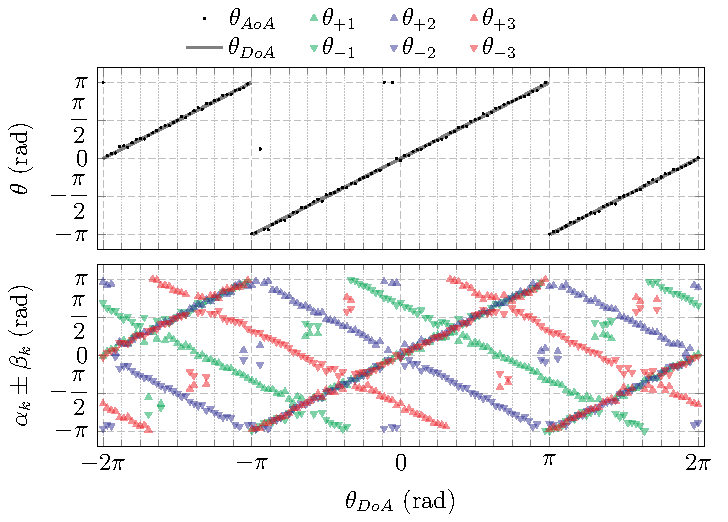
\includegraphics[height=0.785\textheight]{../pictures/simul_POLY_3_R_50_SNR_1.pdf}
			\caption*{\tiny Fonte: Autor, saída gráfica disponível em \href{https://github.com/HeckRodSav/TG/blob/main/documentation/pictures/POLY_3/simul_POLY_3_R_50_SNR_1.gif}{\underline{GitHub}}.}
		\end{figure}
	\end{frame}
	\begin{frame}
		\begin{figure}
			\centering
			\caption*{Caso $\text{SNR} = \SI{0}{\deci\bel}$, com atenuação.}
			% \begin{tikzpicture}
    % \pgfsetfillopacity{0.5}

    \def\fileName{simul_POLY_3_R_50_SNR_1_ATT}
    % \def\fileAddress{../../code/simul/Output/POLY_3/\fileName.dat}
    \def\fileAddress{../data/POLY_3/\fileName.dat}
    % \def\fileAddress{../data/\fileName.dat}

    \def\height{.225\linewidth}
    \def\width{0.75\linewidth}
    \def\distance{0.25cm}
    \def\xmin{-1}
    \def\xmax{101}

    \begin{axis} %configuração do eixo Y esquerdo e eixo X
    [
        name=plot1,
        reverse legend, % inverte a ordem que os items aparecem na legenda
    	% legend style={
        % 	at=(current bounding box.north),
        % 	anchor=south,
        % 	legend columns=6,
        % 	transpose legend,
        % 	draw=none,
        % 	/tikz/every even column/.append style={column sep=0.5cm}
    	% }, % onde exibir
        % axis x line=center,
        % axis y line=center,
        height=\height, % altura da região do gráfico
        width=\width, % largura da região do gráfico
        scale only axis, %
        minor grid style={densely dotted}, % estilo da grade secundária
        major grid style={densely dashed}, % estilo da grade principal
        grid style={lightgray, thin}, % cor das grades
        % axis on top, % forçar grade para ficar por cima do gráfico
        %
        %
        % axis y line*=left, % define gráfico para usar eixo esquerdo sem exibir direito
        y tick label style={
            /pgf/number format/.cd,
            fixed,
            % fixed zerofill,
            precision=1, % quantidade de casas depois da virgula
            /tikz/.cd
        },
        % y filter/.expression={y==0 ? NaN : y},
        scaled y ticks = false,
        ylabel={$\alpha_{k}\pm \beta_{k}$ (\si{\radian})}, % titulo eixo vertical
        % yticklabel={\pgfmathparse{\tick-50}\pgfmathprintnumber{\pgfmathresult}}, % fator multiplicativo para valores do eixo
        y tick label style={/pgf/number format/1000 sep=}, % Altera marcação de milhar
        % yticklabel style={rotate=90},
		ytick={-3.1415, -1.5708, 0, 1.5708, 3.1415},
		yticklabels={$-\pi$,$-\dfrac{\pi}{2}$,$0$,$\dfrac{\pi}{2}$,$\pi$},
        % ytick={0,1,2,3,4,5}, % lista de valores a serem utilizados no eixo
        % ymin=-1,  ymax=4,  % intervalo de valores no eixo y -> na dúvida, deixe comentado
        %
        ymajorgrids=true, % exibir grade principal y
        yminorgrids=true, % exibir grade secundária y
        minor y tick num=4, % contagem de linhas na grade secundária y
        % ybar,
        %
        %
        xlabel={$\theta_{DoA}$ (\si{\radian})}, % título eixo horizontal
        % xticklabel={\pgfmathparse{\tick-50}\pgfmathprintnumber{\pgfmathresult}}, % fator multiplicativo para valores do eixo
        % xticklabels={}, % fator multiplicativo para valores do eixo
		% xtick={0, 12.5, 25, 37.5, 50, 62.6, 75, 87.5, 100},
		% xticklabels={$-2~\pi$,$-\dfrac{3~\pi}{2}$,$-\pi$,$-\dfrac{\pi}{2}$,$0$,$-\dfrac{\pi}{2}$,$\pi$,$-\dfrac{3~\pi}{2}$,$2~\pi$},
		xtick={0, 25, 50, 75, 100},
		xticklabels={$-2 \pi$,$-\pi$,$0$,$\pi$,$2 \pi$},
        % xmode=log,
        % log ticks with fixed point,
        % x filter/.code=\pgfmathparse{#1 + 6.90775527898214},
        x tick label style={
            /pgf/number format/.cd,
            fixed,
            % fixed zerofill,
            precision=1,
            /tikz/.cd,
            /pgf/number format/use comma
        },
        xmin=\xmin, xmax=\xmax, % intervalo de valores no eixo x -> na dúvida, deixe comentado
        scaled x ticks = false,
        %
        xmajorgrids=true, % exibir grade principal x
        xminorgrids=true, % exibir grade secundária x
        minor x tick num=7, % contagem de linhas na grade secundária x
        %
        %
        %
        % unbounded coords=jump,
        % jump threshold/.initial=0.25
    ]

	\addplot[
        antena_3_1,
        mark=triangle*,
		opacity=0.5,
        only marks,
        % smooth
    ] table [
        % col sep=comma,
        x=percent, % cabeçalho da coluna de dados X no arquivo
        y=delta_1_x_3, % cabeçalho da coluna de dados Y no arquivo
    ]
    {\fileAddress};	\label{\fileName.1.1}

    \addplot[
        antena_3_1,
        mark=triangle*,
		opacity=0.5,
		mark options={rotate=180},
        only marks,
        % smooth
    ] table [
        % col sep=comma,
        x=percent, % cabeçalho da coluna de dados X no arquivo
        y=delta_3_x_1, % cabeçalho da coluna de dados Y no arquivo
    ]
    {\fileAddress};	\label{\fileName.1.2}

	\addplot[
        antena_3_2,
        mark=triangle*,
		opacity=0.5,
        only marks,
        % smooth
    ] table [
        % col sep=comma,
        x=percent, % cabeçalho da coluna de dados X no arquivo
        y=delta_2_x_1, % cabeçalho da coluna de dados Y no arquivo
    ]
    {\fileAddress};	\label{\fileName.1.3}

    \addplot[
        antena_3_2,
        mark=triangle*,
		opacity=0.5,
		mark options={rotate=180},
        only marks,
        % smooth
    ] table [
        % col sep=comma,
        x=percent, % cabeçalho da coluna de dados X no arquivo
        y=delta_1_x_2, % cabeçalho da coluna de dados Y no arquivo
    ]
    {\fileAddress};	\label{\fileName.1.4}

	\addplot[
        antena_3_3,
        mark=triangle*,
		opacity=0.5,
        only marks,
        % smooth
    ] table [
        % col sep=comma,
        x=percent, % cabeçalho da coluna de dados X no arquivo
        y=delta_3_x_2, % cabeçalho da coluna de dados Y no arquivo
    ]
    {\fileAddress};	\label{\fileName.1.5}

    \addplot[
        antena_3_3,
        mark=triangle*,
		opacity=0.5,
		mark options={rotate=180},
        only marks,
        % smooth
    ] table [
        % col sep=comma,
        x=percent, % cabeçalho da coluna de dados X no arquivo
        y=delta_2_x_3, % cabeçalho da coluna de dados Y no arquivo
    ]
    {\fileAddress};	\label{\fileName.1.6}

    \end{axis}

    % \begin{axis} %configuração do eixo Y direito e legenda
    % [
    %     legend cell align=left, % alinhamento de texto na legenda
    %     % legend pos={outer north east}, % onde exibir caixa de legenda
    %     % reverse legend, % inverte a ordem que os items aparecem na legenda
    % 	legend style={
    %     	at=(current bounding box.north),
    %     	anchor=south,
    %     	legend columns=2,
    %     % 	transpose legend,
    %     	draw=none
    % 	}, % onde exibir
    %     % axis x line=center,
    %     % axis y line=center,
    %     height=\height, % altura da região do gráfico
    %     width=\width, % largura da região do gráfico
    %     scale only axis, %
    %     minor grid style={densely dotted}, % estilo da grade secundária
    %     major grid style={densely dashed}, % estilo da grade principal
    %     grid style={lightgray, thin}, % cor das grades
    %     % axis on top, % forçar grade para ficar por cima do gráfico
    %     %
    %     %
    %     axis y line*=right, % define gráfico para usar eixo direito sem exibir esquerdo
    %     ylabel={$V_{out}$ (\si{\milli\volt})}, % titulo eixo vertical
    %     y tick label style={
    %         /pgf/number format/.cd,
    %         fixed,
    %         % fixed zerofill,
    %         precision=3, % quantidade de casas depois da virgula
    %         /tikz/.cd,
    %         /pgf/number format/use comma
    %     },
    %     % y filter/.expression={y==0 ? NaN : y},
    %     scaled y ticks = false,
    %     % yticklabel={\pgfmathparse{\tick*10^3}\pgfmathprintnumber{\pgfmathresult}}, % fator multiplicativo para valores do eixo
    %     y tick label style={/pgf/number format/1000 sep=}, % Altera marcação de milhar
    %     % yticklabel style={rotate=90},
    %     % ytick={-12,-6,0,6,12}, % lista de valores a serem utilizados no eixo
    %     % ymin=0.76503, ymax=0.76509,  % intervalo de valores no eixo y -> na dúvida, deixe comentado
    %     %
    %     ymajorgrids=false, % exibir grade principal y
    %     yminorgrids=false, % exibir grade secundária y
    %     minor y tick num=4, % contagem de linhas na grade secundária y
    %     % ybar,
    %     %
    %     %
    %     axis x line=none, %oculta eixo inferior quando o gráfico anterior já exibe
    %     % xlabel={Frequência (\si{\hertz})}, % título eixo horizontal
    %     % xticklabel={\pgfmathparse{\tick*10^3}\pgfmathprintnumber{\pgfmathresult}}, % fator multiplicativo para valores do eixo
    %     % xmode=log,
    %     % log ticks with fixed point,
    %     % x filter/.code=\pgfmathparse{#1 + 6.90775527898214},
    %     % x tick label style={
    %     %     /pgf/number format/.cd,
    %     %     fixed,
    %     %     % fixed zerofill,
    %     %     precision=0,
    %     %     /tikz/.cd,
    %     %     /pgf/number format/use comma
    %     % },
    %     xmin=\xmin, xmax=\xmax, % intervalo de valores no eixo x -> na dúvida, deixe comentado
    %     % scaled x ticks = true,
    %     %
    %     % xmajorgrids=true, % exibir grade principal x
    %     % xminorgrids=true, % exibir grade secundária x
    %     % minor x tick num=7, % contagem de linhas na grade secundária x
    %     %
    %     %
    %     %
    % ]



    % \addplot[mark=none,red, thick]
    % table [
    %     x=time, % cabeçalho da coluna de dados X no arquivo
    %     y=vout % cabeçalho da coluna de dados Y no arquivo
    % ]
    % {graficos/dados/booster.dat};  \label{\fileName.1.2}

    % % \addlegendimage{/pgfplots/refstyle=_1_2}

    % % \addplot[ForestGreen, densely dashdotted, thick]
    % % coordinates
    % % {
    % %     (\pgfkeysvalueof{/pgfplots/xmin},12)
    % %     (\pgfkeysvalueof{/pgfplots/xmax},12)
    % % };
    % % % \addlegendentry{$V_{out}=\pm\SI{12}{\volt}$}

    % % \addplot[ForestGreen, densely dashdotted, thick]
    % % coordinates
    % % {
    % %     (\pgfkeysvalueof{/pgfplots/xmin},-12)
    % %     (\pgfkeysvalueof{/pgfplots/xmax},-12)
    % % };

    % \end{axis}

    \begin{axis} %configuração do eixo Y esquerdo e eixo X
    [
        at={($(plot1.north)+(0,\distance)$)},
        anchor=south,
        % reverse legend, % inverte a ordem que os items aparecem na legenda
		legend style={
        	at=(current bounding box.north),
        	anchor=south,
        	legend columns=2,
        	transpose legend,
        	draw=none,
        	/tikz/every even column/.append style={column sep=0.5cm}
    	}, % onde exibir
        samples=505,
        domain=0:100,
        % axis x line=center,
        % axis y line=center,
        height=\height, % altura da região do gráfico
        width=\width, % largura da região do gráfico
        scale only axis, %
        minor grid style={densely dotted}, % estilo da grade secundária
        major grid style={densely dashed}, % estilo da grade principal
        grid style={lightgray, thin}, % cor das grades
        % axis on top, % forçar grade para ficar por cima do gráfico
        %
        %
        % axis y line*=left, % define gráfico para usar eixo esquerdo sem exibir direito
        y tick label style={
            /pgf/number format/.cd,
            fixed,
            % fixed zerofill,
            precision=1, % quantidade de casas depois da virgula
            /tikz/.cd
        },
        % y filter/.expression={y==0 ? NaN : y},
        scaled y ticks = false,
        ylabel={$\theta$ (\si{\radian})}, % titulo eixo vertical
        % yticklabel={\pgfmathparse{\tick*10^3}\pgfmathprintnumber{\pgfmathresult}}, % fator multiplicativo para valores do eixo
        y tick label style={/pgf/number format/1000 sep=}, % Altera marcação de milhar
        % yticklabel style={rotate=90},
		ytick={-3.1415, -1.5708, 0, 1.5708, 3.1415},
		yticklabels={$-\pi$,$-\dfrac{\pi}{2}$,$0$,$\dfrac{\pi}{2}$,$\pi$},
        % ytick={0,1,2,3,4,5}, % lista de valores a serem utilizados no eixo
        % ymin=-1,  ymax=4,  % intervalo de valores no eixo y -> na dúvida, deixe comentado
        %
        ymajorgrids=true, % exibir grade principal y
        yminorgrids=true, % exibir grade secundária y
        minor y tick num=4, % contagem de linhas na grade secundária y
        % ybar,
        %
        %
        % xlabel={Tempo (\si{\milli\second})}, % título eixo horizontal
        % xticklabel={\pgfmathparse{\tick*10^3}\pgfmathprintnumber{\pgfmathresult}}, % fator multiplicativo para valores do eixo
		xtick={0, 25, 50, 75, 100},
        xticklabels={}, % fator multiplicativo para valores do eixo
        % xmode=log,
        % log ticks with fixed point,
        % x filter/.code=\pgfmathparse{#1 + 6.90775527898214},
        x tick label style={
            /pgf/number format/.cd,
            fixed,
            % fixed zerofill,
            precision=1,
            /tikz/.cd,
            /pgf/number format/use comma
        },
        xmin=\xmin, xmax=\xmax, % intervalo de valores no eixo x -> na dúvida, deixe comentado
        scaled x ticks = false,
        %
        xmajorgrids=true, % exibir grade principal x
        xminorgrids=true, % exibir grade secundária x
        minor x tick num=7, % contagem de linhas na grade secundária x
        %
        %
        %
        unbounded coords=jump,
		jump threshold/.initial=0.01
    ]


    \addplot[
        Black,
        mark=*,
		mark size=0.5pt,
        only marks,
        % smooth
    ] table [
        % col sep=comma,
        x=percent, % cabeçalho da coluna de dados X no arquivo
        y=choose_angle, % cabeçalho da coluna de dados Y no arquivo
	]
	{\fileAddress};	\addlegendentry{$\theta_{AoA}$}

	% \addplot[
	% 	Black,
	% 	mark=o,
	% 	mark size=1.5pt,
	% 	only marks,
	% 	opacity=0.5,
    %     thick,
	% 	% smooth
	% ] table [
	% 	% col sep=comma,
	% 	x=percent, % cabeçalho da coluna de dados X no arquivo
	% 	y=ang_W, % cabeçalho da coluna de dados Y no arquivo
	% ]
	% {\fileAddress};
    \addplot [
        Black,
        opacity=0.5,
        mark=none,
        mark size=5pt,
        very thick,
        % only marks,
        % smooth
    ] {((x==25)||(x==75)?nan:pi*(mod(x+25,50)-25)/25)};
    \addlegendentry{$\theta_{DoA}$}


	\addlegendimage{/pgfplots/refstyle=\fileName.1.1}\addlegendentry{$\theta_{+1}$}
	\addlegendimage{/pgfplots/refstyle=\fileName.1.2}\addlegendentry{$\theta_{-1}$}

	\addlegendimage{/pgfplots/refstyle=\fileName.1.3}\addlegendentry{$\theta_{+2}$}
	\addlegendimage{/pgfplots/refstyle=\fileName.1.4}\addlegendentry{$\theta_{-2}$}

    \addlegendimage{/pgfplots/refstyle=\fileName.1.5}\addlegendentry{$\theta_{+3}$}
	\addlegendimage{/pgfplots/refstyle=\fileName.1.6}\addlegendentry{$\theta_{-3}$}

    \end{axis}

    % \begin{axis} %configuração do eixo Y direito e legenda
    % [
    %     at={($(plot1.north)+(0,\distance)$)},
    %     anchor=south,
    %     legend cell align=left, % alinhamento de texto na legenda
    %     % legend pos={outer north east}, % onde exibir caixa de legenda
    %     % reverse legend, % inverte a ordem que os items aparecem na legenda
    % 	legend style={
    %     	at=(current bounding box.north),
    %     	anchor=south,
    %     	legend columns=3,
    %     % 	transpose legend,
    %     	draw=none,
    %     	/tikz/every even column/.append style={column sep=0.5cm}
    % 	}, % onde exibir
    %     % axis x line=center,
    %     % axis y line=center,
    %     height=\height, % altura da região do gráfico
    %     width=\width, % largura da região do gráfico
    %     scale only axis, %
    %     minor grid style={densely dotted}, % estilo da grade secundária
    %     major grid style={densely dashed}, % estilo da grade principal
    %     grid style={lightgray, thin}, % cor das grades
    %     % axis on top, % forçar grade para ficar por cima do gráfico
    %     %
    %     %
    %     axis y line*=right, % define gráfico para usar eixo direito sem exibir esquerdo
    %     ylabel={$V_{out}$ (\si{\volt})}, % titulo eixo vertical
    %     y tick label style={
    %         /pgf/number format/.cd,
    %         fixed,
    %         % fixed zerofill,
    %         precision=3, % quantidade de casas depois da virgula
    %         /tikz/.cd,
    %         /pgf/number format/use comma
    %     },
    %     % y filter/.expression={y==0 ? NaN : y},
    %     scaled y ticks = false,
    %     % yticklabel={\pgfmathparse{\tick*10^3}\pgfmathprintnumber{\pgfmathresult}}, % fator multiplicativo para valores do eixo
    %     y tick label style={/pgf/number format/1000 sep=}, % Altera marcação de milhar
    %     % yticklabel style={rotate=90},
    %     % ytick={-12,-6,0,6,12}, % lista de valores a serem utilizados no eixo
    %     % ymin=0.76503, ymax=0.76509,  % intervalo de valores no eixo y -> na dúvida, deixe comentado
    %     %
    %     ymajorgrids=false, % exibir grade principal y
    %     yminorgrids=false, % exibir grade secundária y
    %     minor y tick num=4, % contagem de linhas na grade secundária y
    %     % ybar,
    %     %
    %     %
    %     axis x line=none, %oculta eixo inferior quando o gráfico anterior já exibe
    %     % xlabel={Frequência (\si{\hertz})}, % título eixo horizontal
    %     % xticklabel={\pgfmathparse{\tick*10^3}\pgfmathprintnumber{\pgfmathresult}}, % fator multiplicativo para valores do eixo
    %     % xmode=log,
    %     % log ticks with fixed point,
    %     % x filter/.code=\pgfmathparse{#1 + 6.90775527898214},
    %     % x tick label style={
    %     %     /pgf/number format/.cd,
    %     %     fixed,
    %     %     % fixed zerofill,
    %     %     precision=0,
    %     %     /tikz/.cd,
    %     %     /pgf/number format/use comma
    %     % },
    %     xmin=\xmin, xmax=\xmax, % intervalo de valores no eixo x -> na dúvida, deixe comentado
    %     % scaled x ticks = true,
    %     %
    %     % xmajorgrids=true, % exibir grade principal x
    %     % xminorgrids=true, % exibir grade secundária x
    %     % minor x tick num=10, % contagem de linhas na grade secundária x
    %     %
    %     %
    %     %
    % ]


    % \addlegendimage{/pgfplots/refstyle=_2_1}\addlegendentry{$V_{in}$}
    % \addlegendimage{/pgfplots/refstyle=_2_2}\addlegendentry{$V_{in}$}
    % % \addplot[mark=none,red, thick]
    % % table [
    % %     x=time, % cabeçalho da coluna de dados X no arquivo
    % %     y=vout % cabeçalho da coluna de dados Y no arquivo
    % % ]
    % % {graficos/dados/booster.dat}; % \label{\fileName.1.2}
    % % \addlegendentry{$V_{out}$}

    % \addlegendimage{/pgfplots/refstyle=_1_1}\addlegendentry{$I_{out}$}
    % \addlegendimage{/pgfplots/refstyle=_1_2}\addlegendentry{$I_{out}$}

    % % \addlegendimage{/pgfplots/refstyle=_1_2}

    % % \addplot[ForestGreen, densely dashdotted, thick]
    % % coordinates
    % % {
    % %     (\pgfkeysvalueof{/pgfplots/xmin},12)
    % %     (\pgfkeysvalueof{/pgfplots/xmax},12)
    % % };
    % % % \addlegendentry{$V_{out}=\pm\SI{12}{\volt}$}

    % % \addplot[ForestGreen, densely dashdotted, thick]
    % % coordinates
    % % {
    % %     (\pgfkeysvalueof{/pgfplots/xmin},-12)
    % %     (\pgfkeysvalueof{/pgfplots/xmax},-12)
    % % };

    % \end{axis}



\end{tikzpicture}

			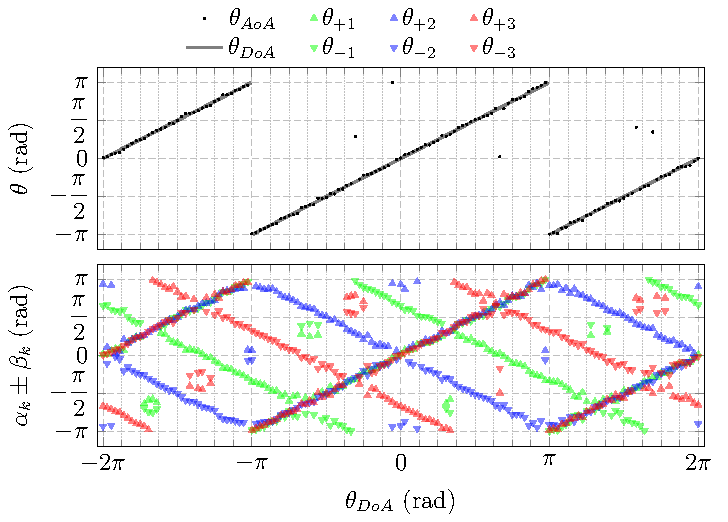
\includegraphics[height=0.785\textheight]{../pictures/simul_POLY_3_R_50_SNR_1_ATT.pdf}
			\caption*{\tiny Fonte: Autor, saída gráfica disponível em \href{https://github.com/HeckRodSav/TG/blob/main/documentation/pictures/POLY_3/simul_POLY_3_R_50_SNR_1_ATT.gif}{\underline{GitHub}}.}
		\end{figure}
	\end{frame}

\subsection{Cinco antenas}
	\begin{frame}{R\textsuperscript{2} para cinco antenas}
		\begin{table}
			\centering
			\begin{tabular}{@{}
				S[table-format = 3.1]
				S[table-format = 3.2, table-model-setup = \bfseries]
				S[table-format = 3.2, table-model-setup = \bfseries]
				@{}}
				\toprule
				{SNR (\unit{\deci\bel})} & {R\textsuperscript{2} sem ATT (\unit{\percent})} & {R\textsuperscript{2} com ATT (\unit{\percent})}
				\\\midrule
				\infinity & \bfseries 100.00 & 100.00\\
				20 & 100.00 & 100.00\\
				17 & 91.90 & 91.89\\
				14 & 91.91 & 91.90\\
				7 & 84.27 & 91.93\\
				0 & \bfseries 80.73 & \bfseries 96.28\\
				\bottomrule
			\end{tabular}
			\caption*{\tiny Fonte: Autor, saídas das simulações disponíveis em \href{https://github.com/HeckRodSav/TG/tree/main/documentation/data/POLY_5}{\underline{GitHub}}.}
		\end{table}
	\end{frame}

	\begin{frame}
		\begin{figure}
			\centering
			\caption*{Caso ideal ($\text{SNR} \rightarrow \qty{\infinity}{\deci\bel}$).}
			% \begin{tikzpicture}
    % \pgfsetfillopacity{0.5}

    \def\fileName{simul_POLY_5_R_50}
    \def\fileAddress{../../code/simul/Output/POLY_5/\fileName.dat}
    % \def\fileAddress{../data/\fileName.dat}

    \def\height{.225\linewidth}
    \def\width{0.75\linewidth}
    \def\distance{0.25cm}
    \def\xmin{-1}
    \def\xmax{101}

    \begin{axis} %configuração do eixo Y esquerdo e eixo X
    [
        name=plot1,
        reverse legend, % inverte a ordem que os items aparecem na legenda
    	% legend style={
        % 	at=(current bounding box.north),
        % 	anchor=south,
        % 	legend columns=6,
        % 	transpose legend,
        % 	draw=none,
        % 	/tikz/every even column/.append style={column sep=0.5cm}
    	% }, % onde exibir
        % axis x line=center,
        % axis y line=center,
        height=\height, % altura da região do gráfico
        width=\width, % largura da região do gráfico
        scale only axis, %
        minor grid style={densely dotted}, % estilo da grade secundária
        major grid style={densely dashed}, % estilo da grade principal
        grid style={lightgray, thin}, % cor das grades
        % axis on top, % forçar grade para ficar por cima do gráfico
        %
        %
        % axis y line*=left, % define gráfico para usar eixo esquerdo sem exibir direito
        y tick label style={
            /pgf/number format/.cd,
            fixed,
            % fixed zerofill,
            precision=1, % quantidade de casas depois da virgula
            /tikz/.cd
        },
        % y filter/.expression={y==0 ? NaN : y},
        scaled y ticks = false,
        ylabel={$\alpha_{k}\pm \beta_{k}$ (\si{\radian})}, % titulo eixo vertical
        % yticklabel={\pgfmathparse{\tick-50}\pgfmathprintnumber{\pgfmathresult}}, % fator multiplicativo para valores do eixo
        y tick label style={/pgf/number format/1000 sep=}, % Altera marcação de milhar
        % yticklabel style={rotate=90},
		ytick={-3.1415, -1.5708, 0, 1.5708, 3.1415},
		yticklabels={$-\pi$,$-\dfrac{\pi}{2}$,$0$,$\dfrac{\pi}{2}$,$\pi$},
        % ytick={0,1,2,3,4,5}, % lista de valores a serem utilizados no eixo
        % ymin=-1,  ymax=4,  % intervalo de valores no eixo y -> na dúvida, deixe comentado
        %
        ymajorgrids=true, % exibir grade principal y
        yminorgrids=true, % exibir grade secundária y
        minor y tick num=4, % contagem de linhas na grade secundária y
        % ybar,
        %
        %
        xlabel={$\theta_{DoA}$ (\si{\radian})}, % título eixo horizontal
        % xticklabel={\pgfmathparse{\tick-50}\pgfmathprintnumber{\pgfmathresult}}, % fator multiplicativo para valores do eixo
        % xticklabels={}, % fator multiplicativo para valores do eixo
		% xtick={0, 12.5, 25, 37.5, 50, 62.6, 75, 87.5, 100},
		% xticklabels={$-2~\pi$,$-\dfrac{3~\pi}{2}$,$-\pi$,$-\dfrac{\pi}{2}$,$0$,$-\dfrac{\pi}{2}$,$\pi$,$-\dfrac{3~\pi}{2}$,$2~\pi$},
		xtick={0, 25, 50, 75, 100},
		xticklabels={$-2 \pi$,$-\pi$,$0$,$\pi$,$2 \pi$},
        % xmode=log,
        % log ticks with fixed point,
        % x filter/.code=\pgfmathparse{#1 + 6.90775527898214},
        x tick label style={
            /pgf/number format/.cd,
            fixed,
            % fixed zerofill,
            precision=1,
            /tikz/.cd,
            /pgf/number format/use comma
        },
        xmin=\xmin, xmax=\xmax, % intervalo de valores no eixo x -> na dúvida, deixe comentado
        scaled x ticks = false,
        %
        xmajorgrids=true, % exibir grade principal x
        xminorgrids=true, % exibir grade secundária x
        minor x tick num=7, % contagem de linhas na grade secundária x
        %
        %
        %
        % unbounded coords=jump,
        % jump threshold/.initial=0.25
    ]

	\addplot[
        cmyk_G,
        mark=triangle*,
		opacity=0.5,
        only marks,
        % smooth
    ] table [
        % col sep=comma,
        x=percent, % cabeçalho da coluna de dados X no arquivo
        y=delta_1_x_5, % cabeçalho da coluna de dados Y no arquivo
    ]
    {\fileAddress};	\label{\fileName.1.1}

    \addplot[
        cmyk_G,
        mark=triangle*,
		opacity=0.5,
		mark options={rotate=180},
        only marks,
        % smooth
    ] table [
        % col sep=comma,
        x=percent, % cabeçalho da coluna de dados X no arquivo
        y=delta_5_x_1, % cabeçalho da coluna de dados Y no arquivo
    ]
    {\fileAddress};	\label{\fileName.1.2}

	\addplot[
        cmyk_B,
        mark=triangle*,
		opacity=0.5,
        only marks,
        % smooth
    ] table [
        % col sep=comma,
        x=percent, % cabeçalho da coluna de dados X no arquivo
        y=delta_2_x_1, % cabeçalho da coluna de dados Y no arquivo
    ]
    {\fileAddress};	\label{\fileName.1.3}

    \addplot[
        cmyk_B,
        mark=triangle*,
		opacity=0.5,
		mark options={rotate=180},
        only marks,
        % smooth
    ] table [
        % col sep=comma,
        x=percent, % cabeçalho da coluna de dados X no arquivo
        y=delta_1_x_2, % cabeçalho da coluna de dados Y no arquivo
    ]
    {\fileAddress};	\label{\fileName.1.4}

	\addplot[
        cmyk_R,
        mark=triangle*,
		opacity=0.5,
        only marks,
        % smooth
    ] table [
        % col sep=comma,
        x=percent, % cabeçalho da coluna de dados X no arquivo
        y=delta_3_x_2, % cabeçalho da coluna de dados Y no arquivo
    ]
    {\fileAddress};	\label{\fileName.1.5}

    \addplot[
        cmyk_R,
        mark=triangle*,
		opacity=0.5,
		mark options={rotate=180},
        only marks,
        % smooth
    ] table [
        % col sep=comma,
        x=percent, % cabeçalho da coluna de dados X no arquivo
        y=delta_2_x_3, % cabeçalho da coluna de dados Y no arquivo
    ]
    {\fileAddress};	\label{\fileName.1.6}

	\addplot[
        cmyk_C,
        mark=triangle*,
		opacity=0.5,
        only marks,
        % smooth
    ] table [
        % col sep=comma,
        x=percent, % cabeçalho da coluna de dados X no arquivo
        y=delta_4_x_3, % cabeçalho da coluna de dados Y no arquivo
    ]
    {\fileAddress};	\label{\fileName.1.7}

    \addplot[
        cmyk_C,
        mark=triangle*,
		opacity=0.5,
		mark options={rotate=180},
        only marks,
        % smooth
    ] table [
        % col sep=comma,
        x=percent, % cabeçalho da coluna de dados X no arquivo
        y=delta_3_x_4, % cabeçalho da coluna de dados Y no arquivo
    ]
    {\fileAddress};	\label{\fileName.1.8}

	\addplot[
        Goldenrod,
        mark=triangle*,
		opacity=0.5,
        only marks,
        % smooth
    ] table [
        % col sep=comma,
        x=percent, % cabeçalho da coluna de dados X no arquivo
        y=delta_5_x_4, % cabeçalho da coluna de dados Y no arquivo
    ]
    {\fileAddress};	\label{\fileName.1.9}

    \addplot[
        Goldenrod,
        mark=triangle*,
		opacity=0.5,
		mark options={rotate=180},
        only marks,
        % smooth
    ] table [
        % col sep=comma,
        x=percent, % cabeçalho da coluna de dados X no arquivo
        y=delta_4_x_5, % cabeçalho da coluna de dados Y no arquivo
    ]
    {\fileAddress};	\label{\fileName.1.10}

    \end{axis}

    % \begin{axis} %configuração do eixo Y direito e legenda
    % [
    %     legend cell align=left, % alinhamento de texto na legenda
    %     % legend pos={outer north east}, % onde exibir caixa de legenda
    %     % reverse legend, % inverte a ordem que os items aparecem na legenda
    % 	legend style={
    %     	at=(current bounding box.north),
    %     	anchor=south,
    %     	legend columns=2,
    %     % 	transpose legend,
    %     	draw=none
    % 	}, % onde exibir
    %     % axis x line=center,
    %     % axis y line=center,
    %     height=\height, % altura da região do gráfico
    %     width=\width, % largura da região do gráfico
    %     scale only axis, %
    %     minor grid style={densely dotted}, % estilo da grade secundária
    %     major grid style={densely dashed}, % estilo da grade principal
    %     grid style={lightgray, thin}, % cor das grades
    %     % axis on top, % forçar grade para ficar por cima do gráfico
    %     %
    %     %
    %     axis y line*=right, % define gráfico para usar eixo direito sem exibir esquerdo
    %     ylabel={$V_{out}$ (\si{\milli\volt})}, % titulo eixo vertical
    %     y tick label style={
    %         /pgf/number format/.cd,
    %         fixed,
    %         % fixed zerofill,
    %         precision=3, % quantidade de casas depois da virgula
    %         /tikz/.cd,
    %         /pgf/number format/use comma
    %     },
    %     % y filter/.expression={y==0 ? NaN : y},
    %     scaled y ticks = false,
    %     % yticklabel={\pgfmathparse{\tick*10^3}\pgfmathprintnumber{\pgfmathresult}}, % fator multiplicativo para valores do eixo
    %     y tick label style={/pgf/number format/1000 sep=}, % Altera marcação de milhar
    %     % yticklabel style={rotate=90},
    %     % ytick={-12,-6,0,6,12}, % lista de valores a serem utilizados no eixo
    %     % ymin=0.76503, ymax=0.76509,  % intervalo de valores no eixo y -> na dúvida, deixe comentado
    %     %
    %     ymajorgrids=false, % exibir grade principal y
    %     yminorgrids=false, % exibir grade secundária y
    %     minor y tick num=4, % contagem de linhas na grade secundária y
    %     % ybar,
    %     %
    %     %
    %     axis x line=none, %oculta eixo inferior quando o gráfico anterior já exibe
    %     % xlabel={Frequência (\si{\hertz})}, % título eixo horizontal
    %     % xticklabel={\pgfmathparse{\tick*10^3}\pgfmathprintnumber{\pgfmathresult}}, % fator multiplicativo para valores do eixo
    %     % xmode=log,
    %     % log ticks with fixed point,
    %     % x filter/.code=\pgfmathparse{#1 + 6.90775527898214},
    %     % x tick label style={
    %     %     /pgf/number format/.cd,
    %     %     fixed,
    %     %     % fixed zerofill,
    %     %     precision=0,
    %     %     /tikz/.cd,
    %     %     /pgf/number format/use comma
    %     % },
    %     xmin=\xmin, xmax=\xmax, % intervalo de valores no eixo x -> na dúvida, deixe comentado
    %     % scaled x ticks = true,
    %     %
    %     % xmajorgrids=true, % exibir grade principal x
    %     % xminorgrids=true, % exibir grade secundária x
    %     % minor x tick num=7, % contagem de linhas na grade secundária x
    %     %
    %     %
    %     %
    % ]



    % \addplot[mark=none,red, thick]
    % table [
    %     x=time, % cabeçalho da coluna de dados X no arquivo
    %     y=vout % cabeçalho da coluna de dados Y no arquivo
    % ]
    % {graficos/dados/booster.dat};  \label{\fileName.1.2}

    % % \addlegendimage{/pgfplots/refstyle=_1_2}

    % % \addplot[ForestGreen, densely dashdotted, thick]
    % % coordinates
    % % {
    % %     (\pgfkeysvalueof{/pgfplots/xmin},12)
    % %     (\pgfkeysvalueof{/pgfplots/xmax},12)
    % % };
    % % % \addlegendentry{$V_{out}=\pm\SI{12}{\volt}$}

    % % \addplot[ForestGreen, densely dashdotted, thick]
    % % coordinates
    % % {
    % %     (\pgfkeysvalueof{/pgfplots/xmin},-12)
    % %     (\pgfkeysvalueof{/pgfplots/xmax},-12)
    % % };

    % \end{axis}

    \begin{axis} %configuração do eixo Y esquerdo e eixo X
    [
        at={($(plot1.north)+(0,\distance)$)},
        anchor=south,
        % reverse legend, % inverte a ordem que os items aparecem na legenda
		legend style={
        	at=(current bounding box.north),
        	anchor=south,
        	legend columns=2,
        	transpose legend,
        	draw=none,
        	/tikz/every even column/.append style={column sep=0.5cm}
    	}, % onde exibir
        samples=505,
        domain=0:100,
        % axis x line=center,
        % axis y line=center,
        height=\height, % altura da região do gráfico
        width=\width, % largura da região do gráfico
        scale only axis, %
        minor grid style={densely dotted}, % estilo da grade secundária
        major grid style={densely dashed}, % estilo da grade principal
        grid style={lightgray, thin}, % cor das grades
        % axis on top, % forçar grade para ficar por cima do gráfico
        %
        %
        % axis y line*=left, % define gráfico para usar eixo esquerdo sem exibir direito
        y tick label style={
            /pgf/number format/.cd,
            fixed,
            % fixed zerofill,
            precision=1, % quantidade de casas depois da virgula
            /tikz/.cd
        },
        % y filter/.expression={y==0 ? NaN : y},
        scaled y ticks = false,
        ylabel={$\theta$ (\si{\radian})}, % titulo eixo vertical
        % yticklabel={\pgfmathparse{\tick*10^3}\pgfmathprintnumber{\pgfmathresult}}, % fator multiplicativo para valores do eixo
        y tick label style={/pgf/number format/1000 sep=}, % Altera marcação de milhar
        % yticklabel style={rotate=90},
		ytick={-3.1415, -1.5708, 0, 1.5708, 3.1415},
		yticklabels={$-\pi$,$-\dfrac{\pi}{2}$,$0$,$\dfrac{\pi}{2}$,$\pi$},
        % ytick={0,1,2,3,4,5}, % lista de valores a serem utilizados no eixo
        % ymin=-1,  ymax=4,  % intervalo de valores no eixo y -> na dúvida, deixe comentado
        %
        ymajorgrids=true, % exibir grade principal y
        yminorgrids=true, % exibir grade secundária y
        minor y tick num=4, % contagem de linhas na grade secundária y
        % ybar,
        %
        %
        % xlabel={Tempo (\si{\milli\second})}, % título eixo horizontal
        % xticklabel={\pgfmathparse{\tick*10^3}\pgfmathprintnumber{\pgfmathresult}}, % fator multiplicativo para valores do eixo
		xtick={0, 25, 50, 75, 100},
        xticklabels={}, % fator multiplicativo para valores do eixo
        % xmode=log,
        % log ticks with fixed point,
        % x filter/.code=\pgfmathparse{#1 + 6.90775527898214},
        x tick label style={
            /pgf/number format/.cd,
            fixed,
            % fixed zerofill,
            precision=1,
            /tikz/.cd,
            /pgf/number format/use comma
        },
        xmin=\xmin, xmax=\xmax, % intervalo de valores no eixo x -> na dúvida, deixe comentado
        scaled x ticks = false,
        %
        xmajorgrids=true, % exibir grade principal x
        xminorgrids=true, % exibir grade secundária x
        minor x tick num=7, % contagem de linhas na grade secundária x
        %
        %
        %
        unbounded coords=jump,
		jump threshold/.initial=0.01
    ]


    \addplot[
        Black,
        mark=*,
		mark size=0.5pt,
        only marks,
        % smooth
    ] table [
        % col sep=comma,
        x=percent, % cabeçalho da coluna de dados X no arquivo
        y=choose_angle, % cabeçalho da coluna de dados Y no arquivo
	]
	{\fileAddress};	\addlegendentry{$\theta_{AoA}$}

	% \addplot[
	% 	Black,
	% 	mark=o,
	% 	mark size=1.5pt,
	% 	only marks,
	% 	opacity=0.5,
    %     thick,
	% 	% smooth
	% ] table [
	% 	% col sep=comma,
	% 	x=percent, % cabeçalho da coluna de dados X no arquivo
	% 	y=ang_W, % cabeçalho da coluna de dados Y no arquivo
	% ]
	% {\fileAddress};
    \addplot [
        Black,
        opacity=0.5,
        mark=none,
        mark size=5pt,
        very thick,
        % only marks,
        % smooth
    ] {((x==25)||(x==75)?nan:pi*(mod(x+25,50)-25)/25)};
    \addlegendentry{$\theta_{DoA}$}


	\addlegendimage{/pgfplots/refstyle=\fileName.1.1}\addlegendentry{$\theta_{+1}$}
	\addlegendimage{/pgfplots/refstyle=\fileName.1.2}\addlegendentry{$\theta_{-1}$}

	\addlegendimage{/pgfplots/refstyle=\fileName.1.3}\addlegendentry{$\theta_{+2}$}
	\addlegendimage{/pgfplots/refstyle=\fileName.1.4}\addlegendentry{$\theta_{-2}$}

    \addlegendimage{/pgfplots/refstyle=\fileName.1.5}\addlegendentry{$\theta_{+3}$}
	\addlegendimage{/pgfplots/refstyle=\fileName.1.6}\addlegendentry{$\theta_{-3}$}

    \addlegendimage{/pgfplots/refstyle=\fileName.1.7}\addlegendentry{$\theta_{+4}$}
	\addlegendimage{/pgfplots/refstyle=\fileName.1.8}\addlegendentry{$\theta_{-4}$}

    \addlegendimage{/pgfplots/refstyle=\fileName.1.9}\addlegendentry{$\theta_{+5}$}
	\addlegendimage{/pgfplots/refstyle=\fileName.1.10}\addlegendentry{$\theta_{-5}$}


    \end{axis}

    % \begin{axis} %configuração do eixo Y direito e legenda
    % [
    %     at={($(plot1.north)+(0,\distance)$)},
    %     anchor=south,
    %     legend cell align=left, % alinhamento de texto na legenda
    %     % legend pos={outer north east}, % onde exibir caixa de legenda
    %     % reverse legend, % inverte a ordem que os items aparecem na legenda
    % 	legend style={
    %     	at=(current bounding box.north),
    %     	anchor=south,
    %     	legend columns=3,
    %     % 	transpose legend,
    %     	draw=none,
    %     	/tikz/every even column/.append style={column sep=0.5cm}
    % 	}, % onde exibir
    %     % axis x line=center,
    %     % axis y line=center,
    %     height=\height, % altura da região do gráfico
    %     width=\width, % largura da região do gráfico
    %     scale only axis, %
    %     minor grid style={densely dotted}, % estilo da grade secundária
    %     major grid style={densely dashed}, % estilo da grade principal
    %     grid style={lightgray, thin}, % cor das grades
    %     % axis on top, % forçar grade para ficar por cima do gráfico
    %     %
    %     %
    %     axis y line*=right, % define gráfico para usar eixo direito sem exibir esquerdo
    %     ylabel={$V_{out}$ (\si{\volt})}, % titulo eixo vertical
    %     y tick label style={
    %         /pgf/number format/.cd,
    %         fixed,
    %         % fixed zerofill,
    %         precision=3, % quantidade de casas depois da virgula
    %         /tikz/.cd,
    %         /pgf/number format/use comma
    %     },
    %     % y filter/.expression={y==0 ? NaN : y},
    %     scaled y ticks = false,
    %     % yticklabel={\pgfmathparse{\tick*10^3}\pgfmathprintnumber{\pgfmathresult}}, % fator multiplicativo para valores do eixo
    %     y tick label style={/pgf/number format/1000 sep=}, % Altera marcação de milhar
    %     % yticklabel style={rotate=90},
    %     % ytick={-12,-6,0,6,12}, % lista de valores a serem utilizados no eixo
    %     % ymin=0.76503, ymax=0.76509,  % intervalo de valores no eixo y -> na dúvida, deixe comentado
    %     %
    %     ymajorgrids=false, % exibir grade principal y
    %     yminorgrids=false, % exibir grade secundária y
    %     minor y tick num=4, % contagem de linhas na grade secundária y
    %     % ybar,
    %     %
    %     %
    %     axis x line=none, %oculta eixo inferior quando o gráfico anterior já exibe
    %     % xlabel={Frequência (\si{\hertz})}, % título eixo horizontal
    %     % xticklabel={\pgfmathparse{\tick*10^3}\pgfmathprintnumber{\pgfmathresult}}, % fator multiplicativo para valores do eixo
    %     % xmode=log,
    %     % log ticks with fixed point,
    %     % x filter/.code=\pgfmathparse{#1 + 6.90775527898214},
    %     % x tick label style={
    %     %     /pgf/number format/.cd,
    %     %     fixed,
    %     %     % fixed zerofill,
    %     %     precision=0,
    %     %     /tikz/.cd,
    %     %     /pgf/number format/use comma
    %     % },
    %     xmin=\xmin, xmax=\xmax, % intervalo de valores no eixo x -> na dúvida, deixe comentado
    %     % scaled x ticks = true,
    %     %
    %     % xmajorgrids=true, % exibir grade principal x
    %     % xminorgrids=true, % exibir grade secundária x
    %     % minor x tick num=10, % contagem de linhas na grade secundária x
    %     %
    %     %
    %     %
    % ]


    % \addlegendimage{/pgfplots/refstyle=_2_1}\addlegendentry{$V_{in}$}
    % \addlegendimage{/pgfplots/refstyle=_2_2}\addlegendentry{$V_{in}$}
    % % \addplot[mark=none,red, thick]
    % % table [
    % %     x=time, % cabeçalho da coluna de dados X no arquivo
    % %     y=vout % cabeçalho da coluna de dados Y no arquivo
    % % ]
    % % {graficos/dados/booster.dat}; % \label{\fileName.1.2}
    % % \addlegendentry{$V_{out}$}

    % \addlegendimage{/pgfplots/refstyle=_1_1}\addlegendentry{$I_{out}$}
    % \addlegendimage{/pgfplots/refstyle=_1_2}\addlegendentry{$I_{out}$}

    % % \addlegendimage{/pgfplots/refstyle=_1_2}

    % % \addplot[ForestGreen, densely dashdotted, thick]
    % % coordinates
    % % {
    % %     (\pgfkeysvalueof{/pgfplots/xmin},12)
    % %     (\pgfkeysvalueof{/pgfplots/xmax},12)
    % % };
    % % % \addlegendentry{$V_{out}=\pm\SI{12}{\volt}$}

    % % \addplot[ForestGreen, densely dashdotted, thick]
    % % coordinates
    % % {
    % %     (\pgfkeysvalueof{/pgfplots/xmin},-12)
    % %     (\pgfkeysvalueof{/pgfplots/xmax},-12)
    % % };

    % \end{axis}



\end{tikzpicture}

			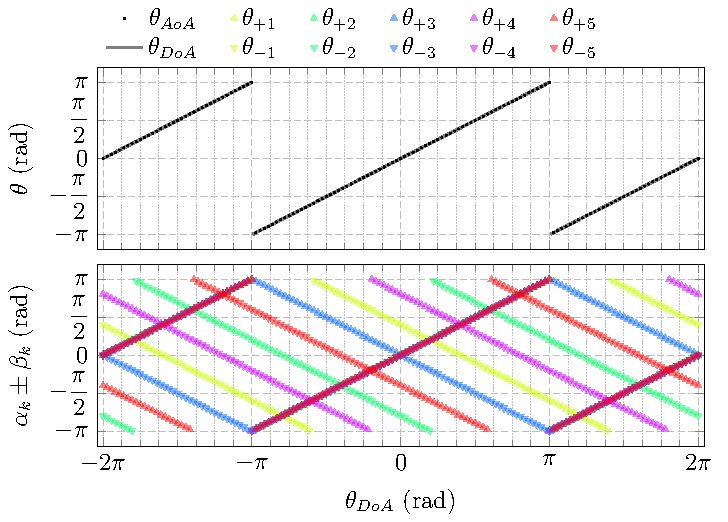
\includegraphics[height=0.785\textheight]{../pictures/simul_POLY_5_R_50.pdf}
			\caption*{\tiny Fonte: Autor, saída gráfica disponível em \href{https://github.com/HeckRodSav/TG/blob/main/documentation/pictures/POLY_5/simul_POLY_5_R_50.gif}{\underline{GitHub}}.}
		\end{figure}
	\end{frame}
	\begin{frame}
		\begin{figure}
			\centering
			\caption*{Caso $\text{SNR} = \SI{0}{\deci\bel}$, sem atenuação.}
			% \begin{tikzpicture}
    % \pgfsetfillopacity{0.5}

    \def\fileName{simul_POLY_5_R_50_SNR_1}
    \def\fileAddress{../../code/simul/Output/POLY_5/\fileName.dat}
    % \def\fileAddress{../data/\fileName.dat}

    \def\height{.225\linewidth}
    \def\width{0.75\linewidth}
    \def\distance{0.25cm}
    \def\xmin{-1}
    \def\xmax{101}

    \begin{axis} %configuração do eixo Y esquerdo e eixo X
    [
        name=plot1,
        reverse legend, % inverte a ordem que os items aparecem na legenda
    	% legend style={
        % 	at=(current bounding box.north),
        % 	anchor=south,
        % 	legend columns=6,
        % 	transpose legend,
        % 	draw=none,
        % 	/tikz/every even column/.append style={column sep=0.5cm}
    	% }, % onde exibir
        % axis x line=center,
        % axis y line=center,
        height=\height, % altura da região do gráfico
        width=\width, % largura da região do gráfico
        scale only axis, %
        minor grid style={densely dotted}, % estilo da grade secundária
        major grid style={densely dashed}, % estilo da grade principal
        grid style={lightgray, thin}, % cor das grades
        % axis on top, % forçar grade para ficar por cima do gráfico
        %
        %
        % axis y line*=left, % define gráfico para usar eixo esquerdo sem exibir direito
        y tick label style={
            /pgf/number format/.cd,
            fixed,
            % fixed zerofill,
            precision=1, % quantidade de casas depois da virgula
            /tikz/.cd
        },
        % y filter/.expression={y==0 ? NaN : y},
        scaled y ticks = false,
        ylabel={$\alpha_{k}\pm \beta_{k}$ (\si{\radian})}, % titulo eixo vertical
        % yticklabel={\pgfmathparse{\tick-50}\pgfmathprintnumber{\pgfmathresult}}, % fator multiplicativo para valores do eixo
        y tick label style={/pgf/number format/1000 sep=}, % Altera marcação de milhar
        % yticklabel style={rotate=90},
		ytick={-3.1415, -1.5708, 0, 1.5708, 3.1415},
		yticklabels={$-\pi$,$-\dfrac{\pi}{2}$,$0$,$\dfrac{\pi}{2}$,$\pi$},
        % ytick={0,1,2,3,4,5}, % lista de valores a serem utilizados no eixo
        % ymin=-1,  ymax=4,  % intervalo de valores no eixo y -> na dúvida, deixe comentado
        %
        ymajorgrids=true, % exibir grade principal y
        yminorgrids=true, % exibir grade secundária y
        minor y tick num=4, % contagem de linhas na grade secundária y
        % ybar,
        %
        %
        xlabel={$\theta_{DoA}$ (\si{\radian})}, % título eixo horizontal
        % xticklabel={\pgfmathparse{\tick-50}\pgfmathprintnumber{\pgfmathresult}}, % fator multiplicativo para valores do eixo
        % xticklabels={}, % fator multiplicativo para valores do eixo
		% xtick={0, 12.5, 25, 37.5, 50, 62.6, 75, 87.5, 100},
		% xticklabels={$-2~\pi$,$-\dfrac{3~\pi}{2}$,$-\pi$,$-\dfrac{\pi}{2}$,$0$,$-\dfrac{\pi}{2}$,$\pi$,$-\dfrac{3~\pi}{2}$,$2~\pi$},
		xtick={0, 25, 50, 75, 100},
		xticklabels={$-2 \pi$,$-\pi$,$0$,$\pi$,$2 \pi$},
        % xmode=log,
        % log ticks with fixed point,
        % x filter/.code=\pgfmathparse{#1 + 6.90775527898214},
        x tick label style={
            /pgf/number format/.cd,
            fixed,
            % fixed zerofill,
            precision=1,
            /tikz/.cd,
            /pgf/number format/use comma
        },
        xmin=\xmin, xmax=\xmax, % intervalo de valores no eixo x -> na dúvida, deixe comentado
        scaled x ticks = false,
        %
        xmajorgrids=true, % exibir grade principal x
        xminorgrids=true, % exibir grade secundária x
        minor x tick num=7, % contagem de linhas na grade secundária x
        %
        %
        %
        % unbounded coords=jump,
        % jump threshold/.initial=0.25
    ]

	\addplot[
        cmyk_G,
        mark=triangle*,
		opacity=0.5,
        only marks,
        % smooth
    ] table [
        % col sep=comma,
        x=percent, % cabeçalho da coluna de dados X no arquivo
        y=delta_1_x_5, % cabeçalho da coluna de dados Y no arquivo
    ]
    {\fileAddress};	\label{\fileName.1.1}

    \addplot[
        cmyk_G,
        mark=triangle*,
		opacity=0.5,
		mark options={rotate=180},
        only marks,
        % smooth
    ] table [
        % col sep=comma,
        x=percent, % cabeçalho da coluna de dados X no arquivo
        y=delta_5_x_1, % cabeçalho da coluna de dados Y no arquivo
    ]
    {\fileAddress};	\label{\fileName.1.2}

	\addplot[
        cmyk_B,
        mark=triangle*,
		opacity=0.5,
        only marks,
        % smooth
    ] table [
        % col sep=comma,
        x=percent, % cabeçalho da coluna de dados X no arquivo
        y=delta_2_x_1, % cabeçalho da coluna de dados Y no arquivo
    ]
    {\fileAddress};	\label{\fileName.1.3}

    \addplot[
        cmyk_B,
        mark=triangle*,
		opacity=0.5,
		mark options={rotate=180},
        only marks,
        % smooth
    ] table [
        % col sep=comma,
        x=percent, % cabeçalho da coluna de dados X no arquivo
        y=delta_1_x_2, % cabeçalho da coluna de dados Y no arquivo
    ]
    {\fileAddress};	\label{\fileName.1.4}

	\addplot[
        cmyk_R,
        mark=triangle*,
		opacity=0.5,
        only marks,
        % smooth
    ] table [
        % col sep=comma,
        x=percent, % cabeçalho da coluna de dados X no arquivo
        y=delta_3_x_2, % cabeçalho da coluna de dados Y no arquivo
    ]
    {\fileAddress};	\label{\fileName.1.5}

    \addplot[
        cmyk_R,
        mark=triangle*,
		opacity=0.5,
		mark options={rotate=180},
        only marks,
        % smooth
    ] table [
        % col sep=comma,
        x=percent, % cabeçalho da coluna de dados X no arquivo
        y=delta_2_x_3, % cabeçalho da coluna de dados Y no arquivo
    ]
    {\fileAddress};	\label{\fileName.1.6}

	\addplot[
        cmyk_C,
        mark=triangle*,
		opacity=0.5,
        only marks,
        % smooth
    ] table [
        % col sep=comma,
        x=percent, % cabeçalho da coluna de dados X no arquivo
        y=delta_4_x_3, % cabeçalho da coluna de dados Y no arquivo
    ]
    {\fileAddress};	\label{\fileName.1.7}

    \addplot[
        cmyk_C,
        mark=triangle*,
		opacity=0.5,
		mark options={rotate=180},
        only marks,
        % smooth
    ] table [
        % col sep=comma,
        x=percent, % cabeçalho da coluna de dados X no arquivo
        y=delta_3_x_4, % cabeçalho da coluna de dados Y no arquivo
    ]
    {\fileAddress};	\label{\fileName.1.8}

	\addplot[
        Goldenrod,
        mark=triangle*,
		opacity=0.5,
        only marks,
        % smooth
    ] table [
        % col sep=comma,
        x=percent, % cabeçalho da coluna de dados X no arquivo
        y=delta_5_x_4, % cabeçalho da coluna de dados Y no arquivo
    ]
    {\fileAddress};	\label{\fileName.1.9}

    \addplot[
        Goldenrod,
        mark=triangle*,
		opacity=0.5,
		mark options={rotate=180},
        only marks,
        % smooth
    ] table [
        % col sep=comma,
        x=percent, % cabeçalho da coluna de dados X no arquivo
        y=delta_4_x_5, % cabeçalho da coluna de dados Y no arquivo
    ]
    {\fileAddress};	\label{\fileName.1.10}

    \end{axis}

    % \begin{axis} %configuração do eixo Y direito e legenda
    % [
    %     legend cell align=left, % alinhamento de texto na legenda
    %     % legend pos={outer north east}, % onde exibir caixa de legenda
    %     % reverse legend, % inverte a ordem que os items aparecem na legenda
    % 	legend style={
    %     	at=(current bounding box.north),
    %     	anchor=south,
    %     	legend columns=2,
    %     % 	transpose legend,
    %     	draw=none
    % 	}, % onde exibir
    %     % axis x line=center,
    %     % axis y line=center,
    %     height=\height, % altura da região do gráfico
    %     width=\width, % largura da região do gráfico
    %     scale only axis, %
    %     minor grid style={densely dotted}, % estilo da grade secundária
    %     major grid style={densely dashed}, % estilo da grade principal
    %     grid style={lightgray, thin}, % cor das grades
    %     % axis on top, % forçar grade para ficar por cima do gráfico
    %     %
    %     %
    %     axis y line*=right, % define gráfico para usar eixo direito sem exibir esquerdo
    %     ylabel={$V_{out}$ (\si{\milli\volt})}, % titulo eixo vertical
    %     y tick label style={
    %         /pgf/number format/.cd,
    %         fixed,
    %         % fixed zerofill,
    %         precision=3, % quantidade de casas depois da virgula
    %         /tikz/.cd,
    %         /pgf/number format/use comma
    %     },
    %     % y filter/.expression={y==0 ? NaN : y},
    %     scaled y ticks = false,
    %     % yticklabel={\pgfmathparse{\tick*10^3}\pgfmathprintnumber{\pgfmathresult}}, % fator multiplicativo para valores do eixo
    %     y tick label style={/pgf/number format/1000 sep=}, % Altera marcação de milhar
    %     % yticklabel style={rotate=90},
    %     % ytick={-12,-6,0,6,12}, % lista de valores a serem utilizados no eixo
    %     % ymin=0.76503, ymax=0.76509,  % intervalo de valores no eixo y -> na dúvida, deixe comentado
    %     %
    %     ymajorgrids=false, % exibir grade principal y
    %     yminorgrids=false, % exibir grade secundária y
    %     minor y tick num=4, % contagem de linhas na grade secundária y
    %     % ybar,
    %     %
    %     %
    %     axis x line=none, %oculta eixo inferior quando o gráfico anterior já exibe
    %     % xlabel={Frequência (\si{\hertz})}, % título eixo horizontal
    %     % xticklabel={\pgfmathparse{\tick*10^3}\pgfmathprintnumber{\pgfmathresult}}, % fator multiplicativo para valores do eixo
    %     % xmode=log,
    %     % log ticks with fixed point,
    %     % x filter/.code=\pgfmathparse{#1 + 6.90775527898214},
    %     % x tick label style={
    %     %     /pgf/number format/.cd,
    %     %     fixed,
    %     %     % fixed zerofill,
    %     %     precision=0,
    %     %     /tikz/.cd,
    %     %     /pgf/number format/use comma
    %     % },
    %     xmin=\xmin, xmax=\xmax, % intervalo de valores no eixo x -> na dúvida, deixe comentado
    %     % scaled x ticks = true,
    %     %
    %     % xmajorgrids=true, % exibir grade principal x
    %     % xminorgrids=true, % exibir grade secundária x
    %     % minor x tick num=7, % contagem de linhas na grade secundária x
    %     %
    %     %
    %     %
    % ]



    % \addplot[mark=none,red, thick]
    % table [
    %     x=time, % cabeçalho da coluna de dados X no arquivo
    %     y=vout % cabeçalho da coluna de dados Y no arquivo
    % ]
    % {graficos/dados/booster.dat};  \label{\fileName.1.2}

    % % \addlegendimage{/pgfplots/refstyle=_1_2}

    % % \addplot[ForestGreen, densely dashdotted, thick]
    % % coordinates
    % % {
    % %     (\pgfkeysvalueof{/pgfplots/xmin},12)
    % %     (\pgfkeysvalueof{/pgfplots/xmax},12)
    % % };
    % % % \addlegendentry{$V_{out}=\pm\SI{12}{\volt}$}

    % % \addplot[ForestGreen, densely dashdotted, thick]
    % % coordinates
    % % {
    % %     (\pgfkeysvalueof{/pgfplots/xmin},-12)
    % %     (\pgfkeysvalueof{/pgfplots/xmax},-12)
    % % };

    % \end{axis}

    \begin{axis} %configuração do eixo Y esquerdo e eixo X
    [
        at={($(plot1.north)+(0,\distance)$)},
        anchor=south,
        % reverse legend, % inverte a ordem que os items aparecem na legenda
		legend style={
        	at=(current bounding box.north),
        	anchor=south,
        	legend columns=2,
        	transpose legend,
        	draw=none,
        	/tikz/every even column/.append style={column sep=0.5cm}
    	}, % onde exibir
        samples=505,
        domain=0:100,
        % axis x line=center,
        % axis y line=center,
        height=\height, % altura da região do gráfico
        width=\width, % largura da região do gráfico
        scale only axis, %
        minor grid style={densely dotted}, % estilo da grade secundária
        major grid style={densely dashed}, % estilo da grade principal
        grid style={lightgray, thin}, % cor das grades
        % axis on top, % forçar grade para ficar por cima do gráfico
        %
        %
        % axis y line*=left, % define gráfico para usar eixo esquerdo sem exibir direito
        y tick label style={
            /pgf/number format/.cd,
            fixed,
            % fixed zerofill,
            precision=1, % quantidade de casas depois da virgula
            /tikz/.cd
        },
        % y filter/.expression={y==0 ? NaN : y},
        scaled y ticks = false,
        ylabel={$\theta$ (\si{\radian})}, % titulo eixo vertical
        % yticklabel={\pgfmathparse{\tick*10^3}\pgfmathprintnumber{\pgfmathresult}}, % fator multiplicativo para valores do eixo
        y tick label style={/pgf/number format/1000 sep=}, % Altera marcação de milhar
        % yticklabel style={rotate=90},
		ytick={-3.1415, -1.5708, 0, 1.5708, 3.1415},
		yticklabels={$-\pi$,$-\dfrac{\pi}{2}$,$0$,$\dfrac{\pi}{2}$,$\pi$},
        % ytick={0,1,2,3,4,5}, % lista de valores a serem utilizados no eixo
        % ymin=-1,  ymax=4,  % intervalo de valores no eixo y -> na dúvida, deixe comentado
        %
        ymajorgrids=true, % exibir grade principal y
        yminorgrids=true, % exibir grade secundária y
        minor y tick num=4, % contagem de linhas na grade secundária y
        % ybar,
        %
        %
        % xlabel={Tempo (\si{\milli\second})}, % título eixo horizontal
        % xticklabel={\pgfmathparse{\tick*10^3}\pgfmathprintnumber{\pgfmathresult}}, % fator multiplicativo para valores do eixo
		xtick={0, 25, 50, 75, 100},
        xticklabels={}, % fator multiplicativo para valores do eixo
        % xmode=log,
        % log ticks with fixed point,
        % x filter/.code=\pgfmathparse{#1 + 6.90775527898214},
        x tick label style={
            /pgf/number format/.cd,
            fixed,
            % fixed zerofill,
            precision=1,
            /tikz/.cd,
            /pgf/number format/use comma
        },
        xmin=\xmin, xmax=\xmax, % intervalo de valores no eixo x -> na dúvida, deixe comentado
        scaled x ticks = false,
        %
        xmajorgrids=true, % exibir grade principal x
        xminorgrids=true, % exibir grade secundária x
        minor x tick num=7, % contagem de linhas na grade secundária x
        %
        %
        %
        unbounded coords=jump,
		jump threshold/.initial=0.01
    ]


    \addplot[
        Black,
        mark=*,
		mark size=0.5pt,
        only marks,
        % smooth
    ] table [
        % col sep=comma,
        x=percent, % cabeçalho da coluna de dados X no arquivo
        y=choose_angle, % cabeçalho da coluna de dados Y no arquivo
	]
	{\fileAddress};	\addlegendentry{$\theta_{AoA}$}

	% \addplot[
	% 	Black,
	% 	mark=o,
	% 	mark size=1.5pt,
	% 	only marks,
	% 	opacity=0.5,
    %     thick,
	% 	% smooth
	% ] table [
	% 	% col sep=comma,
	% 	x=percent, % cabeçalho da coluna de dados X no arquivo
	% 	y=ang_W, % cabeçalho da coluna de dados Y no arquivo
	% ]
	% {\fileAddress};
    \addplot [
        Black,
        opacity=0.5,
        mark=none,
        mark size=5pt,
        very thick,
        % only marks,
        % smooth
    ] {((x==25)||(x==75)?nan:pi*(mod(x+25,50)-25)/25)};
    \addlegendentry{$\theta_{DoA}$}


	\addlegendimage{/pgfplots/refstyle=\fileName.1.1}\addlegendentry{$\theta_{+1}$}
	\addlegendimage{/pgfplots/refstyle=\fileName.1.2}\addlegendentry{$\theta_{-1}$}

	\addlegendimage{/pgfplots/refstyle=\fileName.1.3}\addlegendentry{$\theta_{+2}$}
	\addlegendimage{/pgfplots/refstyle=\fileName.1.4}\addlegendentry{$\theta_{-2}$}

    \addlegendimage{/pgfplots/refstyle=\fileName.1.5}\addlegendentry{$\theta_{+3}$}
	\addlegendimage{/pgfplots/refstyle=\fileName.1.6}\addlegendentry{$\theta_{-3}$}

    \addlegendimage{/pgfplots/refstyle=\fileName.1.7}\addlegendentry{$\theta_{+4}$}
	\addlegendimage{/pgfplots/refstyle=\fileName.1.8}\addlegendentry{$\theta_{-4}$}

    \addlegendimage{/pgfplots/refstyle=\fileName.1.9}\addlegendentry{$\theta_{+5}$}
	\addlegendimage{/pgfplots/refstyle=\fileName.1.10}\addlegendentry{$\theta_{-5}$}


    \end{axis}

    % \begin{axis} %configuração do eixo Y direito e legenda
    % [
    %     at={($(plot1.north)+(0,\distance)$)},
    %     anchor=south,
    %     legend cell align=left, % alinhamento de texto na legenda
    %     % legend pos={outer north east}, % onde exibir caixa de legenda
    %     % reverse legend, % inverte a ordem que os items aparecem na legenda
    % 	legend style={
    %     	at=(current bounding box.north),
    %     	anchor=south,
    %     	legend columns=3,
    %     % 	transpose legend,
    %     	draw=none,
    %     	/tikz/every even column/.append style={column sep=0.5cm}
    % 	}, % onde exibir
    %     % axis x line=center,
    %     % axis y line=center,
    %     height=\height, % altura da região do gráfico
    %     width=\width, % largura da região do gráfico
    %     scale only axis, %
    %     minor grid style={densely dotted}, % estilo da grade secundária
    %     major grid style={densely dashed}, % estilo da grade principal
    %     grid style={lightgray, thin}, % cor das grades
    %     % axis on top, % forçar grade para ficar por cima do gráfico
    %     %
    %     %
    %     axis y line*=right, % define gráfico para usar eixo direito sem exibir esquerdo
    %     ylabel={$V_{out}$ (\si{\volt})}, % titulo eixo vertical
    %     y tick label style={
    %         /pgf/number format/.cd,
    %         fixed,
    %         % fixed zerofill,
    %         precision=3, % quantidade de casas depois da virgula
    %         /tikz/.cd,
    %         /pgf/number format/use comma
    %     },
    %     % y filter/.expression={y==0 ? NaN : y},
    %     scaled y ticks = false,
    %     % yticklabel={\pgfmathparse{\tick*10^3}\pgfmathprintnumber{\pgfmathresult}}, % fator multiplicativo para valores do eixo
    %     y tick label style={/pgf/number format/1000 sep=}, % Altera marcação de milhar
    %     % yticklabel style={rotate=90},
    %     % ytick={-12,-6,0,6,12}, % lista de valores a serem utilizados no eixo
    %     % ymin=0.76503, ymax=0.76509,  % intervalo de valores no eixo y -> na dúvida, deixe comentado
    %     %
    %     ymajorgrids=false, % exibir grade principal y
    %     yminorgrids=false, % exibir grade secundária y
    %     minor y tick num=4, % contagem de linhas na grade secundária y
    %     % ybar,
    %     %
    %     %
    %     axis x line=none, %oculta eixo inferior quando o gráfico anterior já exibe
    %     % xlabel={Frequência (\si{\hertz})}, % título eixo horizontal
    %     % xticklabel={\pgfmathparse{\tick*10^3}\pgfmathprintnumber{\pgfmathresult}}, % fator multiplicativo para valores do eixo
    %     % xmode=log,
    %     % log ticks with fixed point,
    %     % x filter/.code=\pgfmathparse{#1 + 6.90775527898214},
    %     % x tick label style={
    %     %     /pgf/number format/.cd,
    %     %     fixed,
    %     %     % fixed zerofill,
    %     %     precision=0,
    %     %     /tikz/.cd,
    %     %     /pgf/number format/use comma
    %     % },
    %     xmin=\xmin, xmax=\xmax, % intervalo de valores no eixo x -> na dúvida, deixe comentado
    %     % scaled x ticks = true,
    %     %
    %     % xmajorgrids=true, % exibir grade principal x
    %     % xminorgrids=true, % exibir grade secundária x
    %     % minor x tick num=10, % contagem de linhas na grade secundária x
    %     %
    %     %
    %     %
    % ]


    % \addlegendimage{/pgfplots/refstyle=_2_1}\addlegendentry{$V_{in}$}
    % \addlegendimage{/pgfplots/refstyle=_2_2}\addlegendentry{$V_{in}$}
    % % \addplot[mark=none,red, thick]
    % % table [
    % %     x=time, % cabeçalho da coluna de dados X no arquivo
    % %     y=vout % cabeçalho da coluna de dados Y no arquivo
    % % ]
    % % {graficos/dados/booster.dat}; % \label{\fileName.1.2}
    % % \addlegendentry{$V_{out}$}

    % \addlegendimage{/pgfplots/refstyle=_1_1}\addlegendentry{$I_{out}$}
    % \addlegendimage{/pgfplots/refstyle=_1_2}\addlegendentry{$I_{out}$}

    % % \addlegendimage{/pgfplots/refstyle=_1_2}

    % % \addplot[ForestGreen, densely dashdotted, thick]
    % % coordinates
    % % {
    % %     (\pgfkeysvalueof{/pgfplots/xmin},12)
    % %     (\pgfkeysvalueof{/pgfplots/xmax},12)
    % % };
    % % % \addlegendentry{$V_{out}=\pm\SI{12}{\volt}$}

    % % \addplot[ForestGreen, densely dashdotted, thick]
    % % coordinates
    % % {
    % %     (\pgfkeysvalueof{/pgfplots/xmin},-12)
    % %     (\pgfkeysvalueof{/pgfplots/xmax},-12)
    % % };

    % \end{axis}



\end{tikzpicture}

			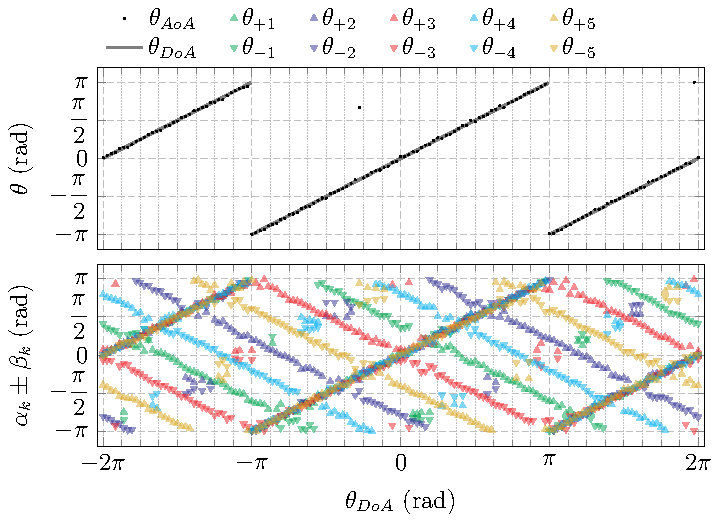
\includegraphics[height=0.785\textheight]{../pictures/simul_POLY_5_R_50_SNR_1.pdf}
			\caption*{\tiny Fonte: Autor, saída gráfica disponível em \href{https://github.com/HeckRodSav/TG/blob/main/documentation/pictures/POLY_5/simul_POLY_5_R_50_SNR_1.gif}{\underline{GitHub}}.}
		\end{figure}
	\end{frame}
	\begin{frame}
		\begin{figure}
			\centering
			\caption*{Caso $\text{SNR} = \SI{0}{\deci\bel}$, com atenuação.}
			% \begin{tikzpicture}
    % \pgfsetfillopacity{0.5}

    \def\fileName{simul_POLY_5_R_50_SNR_1_ATT}
    % \def\fileAddress{../../code/simul/Output/POLY_5/\fileName.dat}
    \def\fileAddress{../data/POLY_5/\fileName.dat}
    % \def\fileAddress{../data/\fileName.dat}

    \def\height{.225\linewidth}
    \def\width{0.75\linewidth}
    \def\distance{0.25cm}
    \def\xmin{-1}
    \def\xmax{101}

    \begin{axis} %configuração do eixo Y esquerdo e eixo X
    [
        name=plot1,
        reverse legend, % inverte a ordem que os items aparecem na legenda
    	% legend style={
        % 	at=(current bounding box.north),
        % 	anchor=south,
        % 	legend columns=6,
        % 	transpose legend,
        % 	draw=none,
        % 	/tikz/every even column/.append style={column sep=0.5cm}
    	% }, % onde exibir
        % axis x line=center,
        % axis y line=center,
        height=\height, % altura da região do gráfico
        width=\width, % largura da região do gráfico
        scale only axis, %
        minor grid style={densely dotted}, % estilo da grade secundária
        major grid style={densely dashed}, % estilo da grade principal
        grid style={lightgray, thin}, % cor das grades
        % axis on top, % forçar grade para ficar por cima do gráfico
        %
        %
        % axis y line*=left, % define gráfico para usar eixo esquerdo sem exibir direito
        y tick label style={
            /pgf/number format/.cd,
            fixed,
            % fixed zerofill,
            precision=1, % quantidade de casas depois da virgula
            /tikz/.cd
        },
        % y filter/.expression={y==0 ? NaN : y},
        scaled y ticks = false,
        ylabel={$\alpha_{k}\pm \beta_{k}$ (\si{\radian})}, % titulo eixo vertical
        % yticklabel={\pgfmathparse{\tick-50}\pgfmathprintnumber{\pgfmathresult}}, % fator multiplicativo para valores do eixo
        y tick label style={/pgf/number format/1000 sep=}, % Altera marcação de milhar
        % yticklabel style={rotate=90},
		ytick={-3.1415, -1.5708, 0, 1.5708, 3.1415},
		yticklabels={$-\pi$,$-\dfrac{\pi}{2}$,$0$,$\dfrac{\pi}{2}$,$\pi$},
        % ytick={0,1,2,3,4,5}, % lista de valores a serem utilizados no eixo
        % ymin=-1,  ymax=4,  % intervalo de valores no eixo y -> na dúvida, deixe comentado
        %
        ymajorgrids=true, % exibir grade principal y
        yminorgrids=true, % exibir grade secundária y
        minor y tick num=4, % contagem de linhas na grade secundária y
        % ybar,
        %
        %
        xlabel={$\theta_{DoA}$ (\si{\radian})}, % título eixo horizontal
        % xticklabel={\pgfmathparse{\tick-50}\pgfmathprintnumber{\pgfmathresult}}, % fator multiplicativo para valores do eixo
        % xticklabels={}, % fator multiplicativo para valores do eixo
		% xtick={0, 12.5, 25, 37.5, 50, 62.6, 75, 87.5, 100},
		% xticklabels={$-2~\pi$,$-\dfrac{3~\pi}{2}$,$-\pi$,$-\dfrac{\pi}{2}$,$0$,$-\dfrac{\pi}{2}$,$\pi$,$-\dfrac{3~\pi}{2}$,$2~\pi$},
		xtick={0, 25, 50, 75, 100},
		xticklabels={$-2 \pi$,$-\pi$,$0$,$\pi$,$2 \pi$},
        % xmode=log,
        % log ticks with fixed point,
        % x filter/.code=\pgfmathparse{#1 + 6.90775527898214},
        x tick label style={
            /pgf/number format/.cd,
            fixed,
            % fixed zerofill,
            precision=1,
            /tikz/.cd,
            /pgf/number format/use comma
        },
        xmin=\xmin, xmax=\xmax, % intervalo de valores no eixo x -> na dúvida, deixe comentado
        scaled x ticks = false,
        %
        xmajorgrids=true, % exibir grade principal x
        xminorgrids=true, % exibir grade secundária x
        minor x tick num=7, % contagem de linhas na grade secundária x
        %
        %
        %
        % unbounded coords=jump,
        % jump threshold/.initial=0.25
    ]

	\addplot[
        cmyk_G,
        mark=triangle*,
		opacity=0.5,
        only marks,
        % smooth
    ] table [
        % col sep=comma,
        x=percent, % cabeçalho da coluna de dados X no arquivo
        y=delta_1_x_5, % cabeçalho da coluna de dados Y no arquivo
    ]
    {\fileAddress};	\label{\fileName.1.1}

    \addplot[
        cmyk_G,
        mark=triangle*,
		opacity=0.5,
		mark options={rotate=180},
        only marks,
        % smooth
    ] table [
        % col sep=comma,
        x=percent, % cabeçalho da coluna de dados X no arquivo
        y=delta_5_x_1, % cabeçalho da coluna de dados Y no arquivo
    ]
    {\fileAddress};	\label{\fileName.1.2}

	\addplot[
        cmyk_B,
        mark=triangle*,
		opacity=0.5,
        only marks,
        % smooth
    ] table [
        % col sep=comma,
        x=percent, % cabeçalho da coluna de dados X no arquivo
        y=delta_2_x_1, % cabeçalho da coluna de dados Y no arquivo
    ]
    {\fileAddress};	\label{\fileName.1.3}

    \addplot[
        cmyk_B,
        mark=triangle*,
		opacity=0.5,
		mark options={rotate=180},
        only marks,
        % smooth
    ] table [
        % col sep=comma,
        x=percent, % cabeçalho da coluna de dados X no arquivo
        y=delta_1_x_2, % cabeçalho da coluna de dados Y no arquivo
    ]
    {\fileAddress};	\label{\fileName.1.4}

	\addplot[
        cmyk_R,
        mark=triangle*,
		opacity=0.5,
        only marks,
        % smooth
    ] table [
        % col sep=comma,
        x=percent, % cabeçalho da coluna de dados X no arquivo
        y=delta_3_x_2, % cabeçalho da coluna de dados Y no arquivo
    ]
    {\fileAddress};	\label{\fileName.1.5}

    \addplot[
        cmyk_R,
        mark=triangle*,
		opacity=0.5,
		mark options={rotate=180},
        only marks,
        % smooth
    ] table [
        % col sep=comma,
        x=percent, % cabeçalho da coluna de dados X no arquivo
        y=delta_2_x_3, % cabeçalho da coluna de dados Y no arquivo
    ]
    {\fileAddress};	\label{\fileName.1.6}

	\addplot[
        cmyk_C,
        mark=triangle*,
		opacity=0.5,
        only marks,
        % smooth
    ] table [
        % col sep=comma,
        x=percent, % cabeçalho da coluna de dados X no arquivo
        y=delta_4_x_3, % cabeçalho da coluna de dados Y no arquivo
    ]
    {\fileAddress};	\label{\fileName.1.7}

    \addplot[
        cmyk_C,
        mark=triangle*,
		opacity=0.5,
		mark options={rotate=180},
        only marks,
        % smooth
    ] table [
        % col sep=comma,
        x=percent, % cabeçalho da coluna de dados X no arquivo
        y=delta_3_x_4, % cabeçalho da coluna de dados Y no arquivo
    ]
    {\fileAddress};	\label{\fileName.1.8}

	\addplot[
        Goldenrod,
        mark=triangle*,
		opacity=0.5,
        only marks,
        % smooth
    ] table [
        % col sep=comma,
        x=percent, % cabeçalho da coluna de dados X no arquivo
        y=delta_5_x_4, % cabeçalho da coluna de dados Y no arquivo
    ]
    {\fileAddress};	\label{\fileName.1.9}

    \addplot[
        Goldenrod,
        mark=triangle*,
		opacity=0.5,
		mark options={rotate=180},
        only marks,
        % smooth
    ] table [
        % col sep=comma,
        x=percent, % cabeçalho da coluna de dados X no arquivo
        y=delta_4_x_5, % cabeçalho da coluna de dados Y no arquivo
    ]
    {\fileAddress};	\label{\fileName.1.10}

    \end{axis}

    % \begin{axis} %configuração do eixo Y direito e legenda
    % [
    %     legend cell align=left, % alinhamento de texto na legenda
    %     % legend pos={outer north east}, % onde exibir caixa de legenda
    %     % reverse legend, % inverte a ordem que os items aparecem na legenda
    % 	legend style={
    %     	at=(current bounding box.north),
    %     	anchor=south,
    %     	legend columns=2,
    %     % 	transpose legend,
    %     	draw=none
    % 	}, % onde exibir
    %     % axis x line=center,
    %     % axis y line=center,
    %     height=\height, % altura da região do gráfico
    %     width=\width, % largura da região do gráfico
    %     scale only axis, %
    %     minor grid style={densely dotted}, % estilo da grade secundária
    %     major grid style={densely dashed}, % estilo da grade principal
    %     grid style={lightgray, thin}, % cor das grades
    %     % axis on top, % forçar grade para ficar por cima do gráfico
    %     %
    %     %
    %     axis y line*=right, % define gráfico para usar eixo direito sem exibir esquerdo
    %     ylabel={$V_{out}$ (\si{\milli\volt})}, % titulo eixo vertical
    %     y tick label style={
    %         /pgf/number format/.cd,
    %         fixed,
    %         % fixed zerofill,
    %         precision=3, % quantidade de casas depois da virgula
    %         /tikz/.cd,
    %         /pgf/number format/use comma
    %     },
    %     % y filter/.expression={y==0 ? NaN : y},
    %     scaled y ticks = false,
    %     % yticklabel={\pgfmathparse{\tick*10^3}\pgfmathprintnumber{\pgfmathresult}}, % fator multiplicativo para valores do eixo
    %     y tick label style={/pgf/number format/1000 sep=}, % Altera marcação de milhar
    %     % yticklabel style={rotate=90},
    %     % ytick={-12,-6,0,6,12}, % lista de valores a serem utilizados no eixo
    %     % ymin=0.76503, ymax=0.76509,  % intervalo de valores no eixo y -> na dúvida, deixe comentado
    %     %
    %     ymajorgrids=false, % exibir grade principal y
    %     yminorgrids=false, % exibir grade secundária y
    %     minor y tick num=4, % contagem de linhas na grade secundária y
    %     % ybar,
    %     %
    %     %
    %     axis x line=none, %oculta eixo inferior quando o gráfico anterior já exibe
    %     % xlabel={Frequência (\si{\hertz})}, % título eixo horizontal
    %     % xticklabel={\pgfmathparse{\tick*10^3}\pgfmathprintnumber{\pgfmathresult}}, % fator multiplicativo para valores do eixo
    %     % xmode=log,
    %     % log ticks with fixed point,
    %     % x filter/.code=\pgfmathparse{#1 + 6.90775527898214},
    %     % x tick label style={
    %     %     /pgf/number format/.cd,
    %     %     fixed,
    %     %     % fixed zerofill,
    %     %     precision=0,
    %     %     /tikz/.cd,
    %     %     /pgf/number format/use comma
    %     % },
    %     xmin=\xmin, xmax=\xmax, % intervalo de valores no eixo x -> na dúvida, deixe comentado
    %     % scaled x ticks = true,
    %     %
    %     % xmajorgrids=true, % exibir grade principal x
    %     % xminorgrids=true, % exibir grade secundária x
    %     % minor x tick num=7, % contagem de linhas na grade secundária x
    %     %
    %     %
    %     %
    % ]



    % \addplot[mark=none,red, thick]
    % table [
    %     x=time, % cabeçalho da coluna de dados X no arquivo
    %     y=vout % cabeçalho da coluna de dados Y no arquivo
    % ]
    % {graficos/dados/booster.dat};  \label{\fileName.1.2}

    % % \addlegendimage{/pgfplots/refstyle=_1_2}

    % % \addplot[ForestGreen, densely dashdotted, thick]
    % % coordinates
    % % {
    % %     (\pgfkeysvalueof{/pgfplots/xmin},12)
    % %     (\pgfkeysvalueof{/pgfplots/xmax},12)
    % % };
    % % % \addlegendentry{$V_{out}=\pm\SI{12}{\volt}$}

    % % \addplot[ForestGreen, densely dashdotted, thick]
    % % coordinates
    % % {
    % %     (\pgfkeysvalueof{/pgfplots/xmin},-12)
    % %     (\pgfkeysvalueof{/pgfplots/xmax},-12)
    % % };

    % \end{axis}

    \begin{axis} %configuração do eixo Y esquerdo e eixo X
    [
        at={($(plot1.north)+(0,\distance)$)},
        anchor=south,
        % reverse legend, % inverte a ordem que os items aparecem na legenda
		legend style={
        	at=(current bounding box.north),
        	anchor=south,
        	legend columns=2,
        	transpose legend,
        	draw=none,
        	/tikz/every even column/.append style={column sep=0.5cm}
    	}, % onde exibir
        samples=505,
        domain=0:100,
        % axis x line=center,
        % axis y line=center,
        height=\height, % altura da região do gráfico
        width=\width, % largura da região do gráfico
        scale only axis, %
        minor grid style={densely dotted}, % estilo da grade secundária
        major grid style={densely dashed}, % estilo da grade principal
        grid style={lightgray, thin}, % cor das grades
        % axis on top, % forçar grade para ficar por cima do gráfico
        %
        %
        % axis y line*=left, % define gráfico para usar eixo esquerdo sem exibir direito
        y tick label style={
            /pgf/number format/.cd,
            fixed,
            % fixed zerofill,
            precision=1, % quantidade de casas depois da virgula
            /tikz/.cd
        },
        % y filter/.expression={y==0 ? NaN : y},
        scaled y ticks = false,
        ylabel={$\theta$ (\si{\radian})}, % titulo eixo vertical
        % yticklabel={\pgfmathparse{\tick*10^3}\pgfmathprintnumber{\pgfmathresult}}, % fator multiplicativo para valores do eixo
        y tick label style={/pgf/number format/1000 sep=}, % Altera marcação de milhar
        % yticklabel style={rotate=90},
		ytick={-3.1415, -1.5708, 0, 1.5708, 3.1415},
		yticklabels={$-\pi$,$-\dfrac{\pi}{2}$,$0$,$\dfrac{\pi}{2}$,$\pi$},
        % ytick={0,1,2,3,4,5}, % lista de valores a serem utilizados no eixo
        % ymin=-1,  ymax=4,  % intervalo de valores no eixo y -> na dúvida, deixe comentado
        %
        ymajorgrids=true, % exibir grade principal y
        yminorgrids=true, % exibir grade secundária y
        minor y tick num=4, % contagem de linhas na grade secundária y
        % ybar,
        %
        %
        % xlabel={Tempo (\si{\milli\second})}, % título eixo horizontal
        % xticklabel={\pgfmathparse{\tick*10^3}\pgfmathprintnumber{\pgfmathresult}}, % fator multiplicativo para valores do eixo
		xtick={0, 25, 50, 75, 100},
        xticklabels={}, % fator multiplicativo para valores do eixo
        % xmode=log,
        % log ticks with fixed point,
        % x filter/.code=\pgfmathparse{#1 + 6.90775527898214},
        x tick label style={
            /pgf/number format/.cd,
            fixed,
            % fixed zerofill,
            precision=1,
            /tikz/.cd,
            /pgf/number format/use comma
        },
        xmin=\xmin, xmax=\xmax, % intervalo de valores no eixo x -> na dúvida, deixe comentado
        scaled x ticks = false,
        %
        xmajorgrids=true, % exibir grade principal x
        xminorgrids=true, % exibir grade secundária x
        minor x tick num=7, % contagem de linhas na grade secundária x
        %
        %
        %
        unbounded coords=jump,
		jump threshold/.initial=0.01
    ]


    \addplot[
        Black,
        mark=*,
		mark size=0.5pt,
        only marks,
        % smooth
    ] table [
        % col sep=comma,
        x=percent, % cabeçalho da coluna de dados X no arquivo
        y=choose_angle, % cabeçalho da coluna de dados Y no arquivo
	]
	{\fileAddress};	\addlegendentry{$\theta_{AoA}$}

	% \addplot[
	% 	Black,
	% 	mark=o,
	% 	mark size=1.5pt,
	% 	only marks,
	% 	opacity=0.5,
    %     thick,
	% 	% smooth
	% ] table [
	% 	% col sep=comma,
	% 	x=percent, % cabeçalho da coluna de dados X no arquivo
	% 	y=ang_W, % cabeçalho da coluna de dados Y no arquivo
	% ]
	% {\fileAddress};
    \addplot [
        Black,
        opacity=0.5,
        mark=none,
        mark size=5pt,
        very thick,
        % only marks,
        % smooth
    ] {((x==25)||(x==75)?nan:pi*(mod(x+25,50)-25)/25)};
    \addlegendentry{$\theta_{DoA}$}


	\addlegendimage{/pgfplots/refstyle=\fileName.1.1}\addlegendentry{$\theta_{+1}$}
	\addlegendimage{/pgfplots/refstyle=\fileName.1.2}\addlegendentry{$\theta_{-1}$}

	\addlegendimage{/pgfplots/refstyle=\fileName.1.3}\addlegendentry{$\theta_{+2}$}
	\addlegendimage{/pgfplots/refstyle=\fileName.1.4}\addlegendentry{$\theta_{-2}$}

    \addlegendimage{/pgfplots/refstyle=\fileName.1.5}\addlegendentry{$\theta_{+3}$}
	\addlegendimage{/pgfplots/refstyle=\fileName.1.6}\addlegendentry{$\theta_{-3}$}

    \addlegendimage{/pgfplots/refstyle=\fileName.1.7}\addlegendentry{$\theta_{+4}$}
	\addlegendimage{/pgfplots/refstyle=\fileName.1.8}\addlegendentry{$\theta_{-4}$}

    \addlegendimage{/pgfplots/refstyle=\fileName.1.9}\addlegendentry{$\theta_{+5}$}
	\addlegendimage{/pgfplots/refstyle=\fileName.1.10}\addlegendentry{$\theta_{-5}$}


    \end{axis}

    % \begin{axis} %configuração do eixo Y direito e legenda
    % [
    %     at={($(plot1.north)+(0,\distance)$)},
    %     anchor=south,
    %     legend cell align=left, % alinhamento de texto na legenda
    %     % legend pos={outer north east}, % onde exibir caixa de legenda
    %     % reverse legend, % inverte a ordem que os items aparecem na legenda
    % 	legend style={
    %     	at=(current bounding box.north),
    %     	anchor=south,
    %     	legend columns=3,
    %     % 	transpose legend,
    %     	draw=none,
    %     	/tikz/every even column/.append style={column sep=0.5cm}
    % 	}, % onde exibir
    %     % axis x line=center,
    %     % axis y line=center,
    %     height=\height, % altura da região do gráfico
    %     width=\width, % largura da região do gráfico
    %     scale only axis, %
    %     minor grid style={densely dotted}, % estilo da grade secundária
    %     major grid style={densely dashed}, % estilo da grade principal
    %     grid style={lightgray, thin}, % cor das grades
    %     % axis on top, % forçar grade para ficar por cima do gráfico
    %     %
    %     %
    %     axis y line*=right, % define gráfico para usar eixo direito sem exibir esquerdo
    %     ylabel={$V_{out}$ (\si{\volt})}, % titulo eixo vertical
    %     y tick label style={
    %         /pgf/number format/.cd,
    %         fixed,
    %         % fixed zerofill,
    %         precision=3, % quantidade de casas depois da virgula
    %         /tikz/.cd,
    %         /pgf/number format/use comma
    %     },
    %     % y filter/.expression={y==0 ? NaN : y},
    %     scaled y ticks = false,
    %     % yticklabel={\pgfmathparse{\tick*10^3}\pgfmathprintnumber{\pgfmathresult}}, % fator multiplicativo para valores do eixo
    %     y tick label style={/pgf/number format/1000 sep=}, % Altera marcação de milhar
    %     % yticklabel style={rotate=90},
    %     % ytick={-12,-6,0,6,12}, % lista de valores a serem utilizados no eixo
    %     % ymin=0.76503, ymax=0.76509,  % intervalo de valores no eixo y -> na dúvida, deixe comentado
    %     %
    %     ymajorgrids=false, % exibir grade principal y
    %     yminorgrids=false, % exibir grade secundária y
    %     minor y tick num=4, % contagem de linhas na grade secundária y
    %     % ybar,
    %     %
    %     %
    %     axis x line=none, %oculta eixo inferior quando o gráfico anterior já exibe
    %     % xlabel={Frequência (\si{\hertz})}, % título eixo horizontal
    %     % xticklabel={\pgfmathparse{\tick*10^3}\pgfmathprintnumber{\pgfmathresult}}, % fator multiplicativo para valores do eixo
    %     % xmode=log,
    %     % log ticks with fixed point,
    %     % x filter/.code=\pgfmathparse{#1 + 6.90775527898214},
    %     % x tick label style={
    %     %     /pgf/number format/.cd,
    %     %     fixed,
    %     %     % fixed zerofill,
    %     %     precision=0,
    %     %     /tikz/.cd,
    %     %     /pgf/number format/use comma
    %     % },
    %     xmin=\xmin, xmax=\xmax, % intervalo de valores no eixo x -> na dúvida, deixe comentado
    %     % scaled x ticks = true,
    %     %
    %     % xmajorgrids=true, % exibir grade principal x
    %     % xminorgrids=true, % exibir grade secundária x
    %     % minor x tick num=10, % contagem de linhas na grade secundária x
    %     %
    %     %
    %     %
    % ]


    % \addlegendimage{/pgfplots/refstyle=_2_1}\addlegendentry{$V_{in}$}
    % \addlegendimage{/pgfplots/refstyle=_2_2}\addlegendentry{$V_{in}$}
    % % \addplot[mark=none,red, thick]
    % % table [
    % %     x=time, % cabeçalho da coluna de dados X no arquivo
    % %     y=vout % cabeçalho da coluna de dados Y no arquivo
    % % ]
    % % {graficos/dados/booster.dat}; % \label{\fileName.1.2}
    % % \addlegendentry{$V_{out}$}

    % \addlegendimage{/pgfplots/refstyle=_1_1}\addlegendentry{$I_{out}$}
    % \addlegendimage{/pgfplots/refstyle=_1_2}\addlegendentry{$I_{out}$}

    % % \addlegendimage{/pgfplots/refstyle=_1_2}

    % % \addplot[ForestGreen, densely dashdotted, thick]
    % % coordinates
    % % {
    % %     (\pgfkeysvalueof{/pgfplots/xmin},12)
    % %     (\pgfkeysvalueof{/pgfplots/xmax},12)
    % % };
    % % % \addlegendentry{$V_{out}=\pm\SI{12}{\volt}$}

    % % \addplot[ForestGreen, densely dashdotted, thick]
    % % coordinates
    % % {
    % %     (\pgfkeysvalueof{/pgfplots/xmin},-12)
    % %     (\pgfkeysvalueof{/pgfplots/xmax},-12)
    % % };

    % \end{axis}



\end{tikzpicture}

			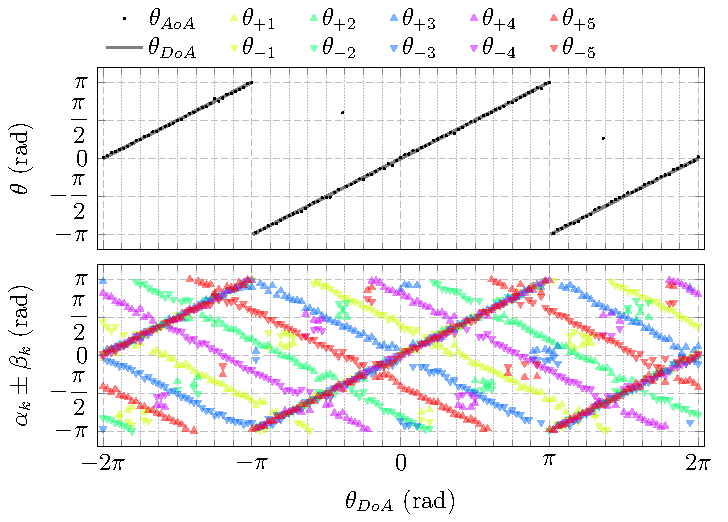
\includegraphics[height=0.785\textheight]{../pictures/simul_POLY_5_R_50_SNR_1_ATT.pdf}
			\caption*{\tiny Fonte: Autor, saída gráfica disponível em \href{https://github.com/HeckRodSav/TG/blob/main/documentation/pictures/POLY_5/simul_POLY_5_R_50_SNR_1_ATT.gif}{\underline{GitHub}}.}
		\end{figure}
	\end{frame}

\subsection{Setes antenas}
	\begin{frame}{R\textsuperscript{2} para sete antenas}
		\begin{table}
			\centering
			\begin{tabular}{@{}
			S[table-format = 3.1]
			S[table-format = 3.2, table-model-setup = \bfseries]
			S[table-format = 3.2, table-model-setup = \bfseries]
			@{}}
			\toprule
			{SNR (\unit{\deci\bel})} & {R\textsuperscript{2} sem ATT (\unit{\percent})} & {R\textsuperscript{2} com ATT (\unit{\percent})}
			\\\midrule
			\infinity & \bfseries 100.00 & 100.00\\
			20 & 84.25 & 100.00\\
			17 & 100.00 & 84.24\\
			14 & 91.90 & 100.00\\
			7 & 99.99 & 84.28\\
			0 & \bfseries 80.15 & \bfseries 99.98\\
			\bottomrule
		\end{tabular}
		\caption*{\tiny Fonte: Autor, saídas das simulações disponíveis em \href{https://github.com/HeckRodSav/TG/tree/main/documentation/data/POLY_7}{\underline{GitHub}}.}
	\end{table}
	\end{frame}

	\begin{frame}
		\begin{figure}
			\centering
			\caption*{Caso ideal ($\text{SNR} \rightarrow \qty{\infinity}{\deci\bel}$).}
			% \begin{tikzpicture}
    % \pgfsetfillopacity{0.5}

    \def\fileName{simul_POLY_7_R_50}
    % \def\fileAddress{../../code/simul/Output/POLY_7/\fileName.dat}
    \def\fileAddress{../data/POLY_7/\fileName.dat}
    % \def\fileAddress{../data/\fileName.dat}

    \def\height{.225\linewidth}
    \def\width{0.75\linewidth}
    \def\distance{0.25cm}
    \def\xmin{-1}
    \def\xmax{101}

    \begin{axis} %configuração do eixo Y esquerdo e eixo X
    [
        name=plot1,
        reverse legend, % inverte a ordem que os items aparecem na legenda
    	% legend style={
        % 	at=(current bounding box.north),
        % 	anchor=south,
        % 	legend columns=6,
        % 	transpose legend,
        % 	draw=none,
        % 	/tikz/every even column/.append style={column sep=0.5cm}
    	% }, % onde exibir
        % axis x line=center,
        % axis y line=center,
        height=\height, % altura da região do gráfico
        width=\width, % largura da região do gráfico
        scale only axis, %
        minor grid style={densely dotted}, % estilo da grade secundária
        major grid style={densely dashed}, % estilo da grade principal
        grid style={lightgray, thin}, % cor das grades
        % axis on top, % forçar grade para ficar por cima do gráfico
        %
        %
        % axis y line*=left, % define gráfico para usar eixo esquerdo sem exibir direito
        y tick label style={
            /pgf/number format/.cd,
            fixed,
            % fixed zerofill,
            precision=1, % quantidade de casas depois da virgula
            /tikz/.cd
        },
        % y filter/.expression={y==0 ? NaN : y},
        scaled y ticks = false,
        ylabel={$\alpha_{k}\pm \beta_{k}$ (\si{\radian})}, % titulo eixo vertical
        % yticklabel={\pgfmathparse{\tick-50}\pgfmathprintnumber{\pgfmathresult}}, % fator multiplicativo para valores do eixo
        y tick label style={/pgf/number format/1000 sep=}, % Altera marcação de milhar
        % yticklabel style={rotate=90},
		ytick={-3.1415, -1.5708, 0, 1.5708, 3.1415},
		yticklabels={$-\pi$,$-\dfrac{\pi}{2}$,$0$,$\dfrac{\pi}{2}$,$\pi$},
        % ytick={0,1,2,3,4,5}, % lista de valores a serem utilizados no eixo
        % ymin=-1,  ymax=4,  % intervalo de valores no eixo y -> na dúvida, deixe comentado
        %
        ymajorgrids=true, % exibir grade principal y
        yminorgrids=true, % exibir grade secundária y
        minor y tick num=4, % contagem de linhas na grade secundária y
        % ybar,
        %
        %
        xlabel={$\theta_{DoA}$ (\si{\radian})}, % título eixo horizontal
        % xticklabel={\pgfmathparse{\tick-50}\pgfmathprintnumber{\pgfmathresult}}, % fator multiplicativo para valores do eixo
        % xticklabels={}, % fator multiplicativo para valores do eixo
		% xtick={0, 12.5, 25, 37.5, 50, 62.6, 75, 87.5, 100},
		% xticklabels={$-2~\pi$,$-\dfrac{3~\pi}{2}$,$-\pi$,$-\dfrac{\pi}{2}$,$0$,$-\dfrac{\pi}{2}$,$\pi$,$-\dfrac{3~\pi}{2}$,$2~\pi$},
		xtick={0, 25, 50, 75, 100},
		xticklabels={$-2 \pi$,$-\pi$,$0$,$\pi$,$2 \pi$},
        % xmode=log,
        % log ticks with fixed point,
        % x filter/.code=\pgfmathparse{#1 + 6.90775527898214},
        x tick label style={
            /pgf/number format/.cd,
            fixed,
            % fixed zerofill,
            precision=1,
            /tikz/.cd,
            /pgf/number format/use comma
        },
        xmin=\xmin, xmax=\xmax, % intervalo de valores no eixo x -> na dúvida, deixe comentado
        scaled x ticks = false,
        %
        xmajorgrids=true, % exibir grade principal x
        xminorgrids=true, % exibir grade secundária x
        minor x tick num=7, % contagem de linhas na grade secundária x
        %
        %
        %
        % unbounded coords=jump,
        % jump threshold/.initial=0.25
    ]

	\addplot[
        antena_7_1,
        mark=triangle*,
		opacity=0.5,
        only marks,
        % smooth
    ] table [
        % col sep=comma,
        x=percent, % cabeçalho da coluna de dados X no arquivo
        y=delta_1_x_7, % cabeçalho da coluna de dados Y no arquivo
    ]
    {\fileAddress};	\label{\fileName.1.1}

    \addplot[
        antena_7_1,
        mark=triangle*,
		opacity=0.5,
		mark options={rotate=180},
        only marks,
        % smooth
    ] table [
        % col sep=comma,
        x=percent, % cabeçalho da coluna de dados X no arquivo
        y=delta_7_x_1, % cabeçalho da coluna de dados Y no arquivo
    ]
    {\fileAddress};	\label{\fileName.1.2}

	\addplot[
        antena_7_2,
        mark=triangle*,
		opacity=0.5,
        only marks,
        % smooth
    ] table [
        % col sep=comma,
        x=percent, % cabeçalho da coluna de dados X no arquivo
        y=delta_2_x_1, % cabeçalho da coluna de dados Y no arquivo
    ]
    {\fileAddress};	\label{\fileName.1.3}

    \addplot[
        antena_7_2,
        mark=triangle*,
		opacity=0.5,
		mark options={rotate=180},
        only marks,
        % smooth
    ] table [
        % col sep=comma,
        x=percent, % cabeçalho da coluna de dados X no arquivo
        y=delta_1_x_2, % cabeçalho da coluna de dados Y no arquivo
    ]
    {\fileAddress};	\label{\fileName.1.4}

	\addplot[
        antena_7_3,
        mark=triangle*,
		opacity=0.5,
        only marks,
        % smooth
    ] table [
        % col sep=comma,
        x=percent, % cabeçalho da coluna de dados X no arquivo
        y=delta_3_x_2, % cabeçalho da coluna de dados Y no arquivo
    ]
    {\fileAddress};	\label{\fileName.1.5}

    \addplot[
        antena_7_3,
        mark=triangle*,
		opacity=0.5,
		mark options={rotate=180},
        only marks,
        % smooth
    ] table [
        % col sep=comma,
        x=percent, % cabeçalho da coluna de dados X no arquivo
        y=delta_2_x_3, % cabeçalho da coluna de dados Y no arquivo
    ]
    {\fileAddress};	\label{\fileName.1.6}

	\addplot[
        antena_7_4,
        mark=triangle*,
		opacity=0.5,
        only marks,
        % smooth
    ] table [
        % col sep=comma,
        x=percent, % cabeçalho da coluna de dados X no arquivo
        y=delta_4_x_3, % cabeçalho da coluna de dados Y no arquivo
    ]
    {\fileAddress};	\label{\fileName.1.7}

    \addplot[
        antena_7_4,
        mark=triangle*,
		opacity=0.5,
		mark options={rotate=180},
        only marks,
        % smooth
    ] table [
        % col sep=comma,
        x=percent, % cabeçalho da coluna de dados X no arquivo
        y=delta_3_x_4, % cabeçalho da coluna de dados Y no arquivo
    ]
    {\fileAddress};	\label{\fileName.1.8}

	\addplot[
        antena_7_5,
        mark=triangle*,
		opacity=0.5,
        only marks,
        % smooth
    ] table [
        % col sep=comma,
        x=percent, % cabeçalho da coluna de dados X no arquivo
        y=delta_5_x_4, % cabeçalho da coluna de dados Y no arquivo
    ]
    {\fileAddress};	\label{\fileName.1.9}

    \addplot[
        antena_7_5,
        mark=triangle*,
		opacity=0.5,
		mark options={rotate=180},
        only marks,
        % smooth
    ] table [
        % col sep=comma,
        x=percent, % cabeçalho da coluna de dados X no arquivo
        y=delta_4_x_5, % cabeçalho da coluna de dados Y no arquivo
    ]
    {\fileAddress};	\label{\fileName.1.10}

	\addplot[
        antena_7_6,
        mark=triangle*,
		opacity=0.5,
        only marks,
        % smooth
    ] table [
        % col sep=comma,
        x=percent, % cabeçalho da coluna de dados X no arquivo
        y=delta_6_x_5, % cabeçalho da coluna de dados Y no arquivo
    ]
    {\fileAddress};	\label{\fileName.1.11}

    \addplot[
        antena_7_6,
        mark=triangle*,
		opacity=0.5,
		mark options={rotate=180},
        only marks,
        % smooth
    ] table [
        % col sep=comma,
        x=percent, % cabeçalho da coluna de dados X no arquivo
        y=delta_5_x_6 % cabeçalho da coluna de dados Y no arquivo
    ]
    {\fileAddress};	\label{\fileName.1.12}

	\addplot[
        antena_7_7,
        mark=triangle*,
		opacity=0.5,
        only marks,
        % smooth
    ] table [
        % col sep=comma,
        x=percent, % cabeçalho da coluna de dados X no arquivo
        y=delta_7_x_6, % cabeçalho da coluna de dados Y no arquivo
    ]
    {\fileAddress};	\label{\fileName.1.13}

    \addplot[
        antena_7_7,
        mark=triangle*,
		opacity=0.5,
		mark options={rotate=180},
        only marks,
        % smooth
    ] table [
        % col sep=comma,
        x=percent, % cabeçalho da coluna de dados X no arquivo
        y=delta_6_x_7, % cabeçalho da coluna de dados Y no arquivo
    ]
    {\fileAddress};	\label{\fileName.1.14}

    \end{axis}

    % \begin{axis} %configuração do eixo Y direito e legenda
    % [
    %     legend cell align=left, % alinhamento de texto na legenda
    %     % legend pos={outer north east}, % onde exibir caixa de legenda
    %     % reverse legend, % inverte a ordem que os items aparecem na legenda
    % 	legend style={
    %     	at=(current bounding box.north),
    %     	anchor=south,
    %     	legend columns=2,
    %     % 	transpose legend,
    %     	draw=none
    % 	}, % onde exibir
    %     % axis x line=center,
    %     % axis y line=center,
    %     height=\height, % altura da região do gráfico
    %     width=\width, % largura da região do gráfico
    %     scale only axis, %
    %     minor grid style={densely dotted}, % estilo da grade secundária
    %     major grid style={densely dashed}, % estilo da grade principal
    %     grid style={lightgray, thin}, % cor das grades
    %     % axis on top, % forçar grade para ficar por cima do gráfico
    %     %
    %     %
    %     axis y line*=right, % define gráfico para usar eixo direito sem exibir esquerdo
    %     ylabel={$V_{out}$ (\si{\milli\volt})}, % titulo eixo vertical
    %     y tick label style={
    %         /pgf/number format/.cd,
    %         fixed,
    %         % fixed zerofill,
    %         precision=3, % quantidade de casas depois da virgula
    %         /tikz/.cd,
    %         /pgf/number format/use comma
    %     },
    %     % y filter/.expression={y==0 ? NaN : y},
    %     scaled y ticks = false,
    %     % yticklabel={\pgfmathparse{\tick*10^3}\pgfmathprintnumber{\pgfmathresult}}, % fator multiplicativo para valores do eixo
    %     y tick label style={/pgf/number format/1000 sep=}, % Altera marcação de milhar
    %     % yticklabel style={rotate=90},
    %     % ytick={-12,-6,0,6,12}, % lista de valores a serem utilizados no eixo
    %     % ymin=0.76503, ymax=0.76509,  % intervalo de valores no eixo y -> na dúvida, deixe comentado
    %     %
    %     ymajorgrids=false, % exibir grade principal y
    %     yminorgrids=false, % exibir grade secundária y
    %     minor y tick num=4, % contagem de linhas na grade secundária y
    %     % ybar,
    %     %
    %     %
    %     axis x line=none, %oculta eixo inferior quando o gráfico anterior já exibe
    %     % xlabel={Frequência (\si{\hertz})}, % título eixo horizontal
    %     % xticklabel={\pgfmathparse{\tick*10^3}\pgfmathprintnumber{\pgfmathresult}}, % fator multiplicativo para valores do eixo
    %     % xmode=log,
    %     % log ticks with fixed point,
    %     % x filter/.code=\pgfmathparse{#1 + 6.90775527898214},
    %     % x tick label style={
    %     %     /pgf/number format/.cd,
    %     %     fixed,
    %     %     % fixed zerofill,
    %     %     precision=0,
    %     %     /tikz/.cd,
    %     %     /pgf/number format/use comma
    %     % },
    %     xmin=\xmin, xmax=\xmax, % intervalo de valores no eixo x -> na dúvida, deixe comentado
    %     % scaled x ticks = true,
    %     %
    %     % xmajorgrids=true, % exibir grade principal x
    %     % xminorgrids=true, % exibir grade secundária x
    %     % minor x tick num=7, % contagem de linhas na grade secundária x
    %     %
    %     %
    %     %
    % ]



    % \addplot[mark=none,red, thick]
    % table [
    %     x=time, % cabeçalho da coluna de dados X no arquivo
    %     y=vout % cabeçalho da coluna de dados Y no arquivo
    % ]
    % {graficos/dados/booster.dat};  \label{\fileName.1.2}

    % % \addlegendimage{/pgfplots/refstyle=_1_2}

    % % \addplot[ForestGreen, densely dashdotted, thick]
    % % coordinates
    % % {
    % %     (\pgfkeysvalueof{/pgfplots/xmin},12)
    % %     (\pgfkeysvalueof{/pgfplots/xmax},12)
    % % };
    % % % \addlegendentry{$V_{out}=\pm\SI{12}{\volt}$}

    % % \addplot[ForestGreen, densely dashdotted, thick]
    % % coordinates
    % % {
    % %     (\pgfkeysvalueof{/pgfplots/xmin},-12)
    % %     (\pgfkeysvalueof{/pgfplots/xmax},-12)
    % % };

    % \end{axis}

    \begin{axis} %configuração do eixo Y esquerdo e eixo X
    [
        at={($(plot1.north)+(0,\distance)$)},
        anchor=south,
        % reverse legend, % inverte a ordem que os items aparecem na legenda
		legend style={
        	at=(current bounding box.north),
        	anchor=south,
        	legend columns=2,
        	transpose legend,
        	draw=none,
        	/tikz/every even column/.append style={column sep=0.5cm}
    	}, % onde exibir
        samples=505,
        domain=0:100,
        % axis x line=center,
        % axis y line=center,
        height=\height, % altura da região do gráfico
        width=\width, % largura da região do gráfico
        scale only axis, %
        minor grid style={densely dotted}, % estilo da grade secundária
        major grid style={densely dashed}, % estilo da grade principal
        grid style={lightgray, thin}, % cor das grades
        % axis on top, % forçar grade para ficar por cima do gráfico
        %
        %
        % axis y line*=left, % define gráfico para usar eixo esquerdo sem exibir direito
        y tick label style={
            /pgf/number format/.cd,
            fixed,
            % fixed zerofill,
            precision=1, % quantidade de casas depois da virgula
            /tikz/.cd
        },
        % y filter/.expression={y==0 ? NaN : y},
        scaled y ticks = false,
        ylabel={$\theta$ (\si{\radian})}, % titulo eixo vertical
        % yticklabel={\pgfmathparse{\tick*10^3}\pgfmathprintnumber{\pgfmathresult}}, % fator multiplicativo para valores do eixo
        y tick label style={/pgf/number format/1000 sep=}, % Altera marcação de milhar
        % yticklabel style={rotate=90},
		ytick={-3.1415, -1.5708, 0, 1.5708, 3.1415},
		yticklabels={$-\pi$,$-\dfrac{\pi}{2}$,$0$,$\dfrac{\pi}{2}$,$\pi$},
        % ytick={0,1,2,3,4,5}, % lista de valores a serem utilizados no eixo
        % ymin=-1,  ymax=4,  % intervalo de valores no eixo y -> na dúvida, deixe comentado
        %
        ymajorgrids=true, % exibir grade principal y
        yminorgrids=true, % exibir grade secundária y
        minor y tick num=4, % contagem de linhas na grade secundária y
        % ybar,
        %
        %
        % xlabel={Tempo (\si{\milli\second})}, % título eixo horizontal
        % xticklabel={\pgfmathparse{\tick*10^3}\pgfmathprintnumber{\pgfmathresult}}, % fator multiplicativo para valores do eixo
		xtick={0, 25, 50, 75, 100},
        xticklabels={}, % fator multiplicativo para valores do eixo
        % xmode=log,
        % log ticks with fixed point,
        % x filter/.code=\pgfmathparse{#1 + 6.90775527898214},
        x tick label style={
            /pgf/number format/.cd,
            fixed,
            % fixed zerofill,
            precision=1,
            /tikz/.cd,
            /pgf/number format/use comma
        },
        xmin=\xmin, xmax=\xmax, % intervalo de valores no eixo x -> na dúvida, deixe comentado
        scaled x ticks = false,
        %
        xmajorgrids=true, % exibir grade principal x
        xminorgrids=true, % exibir grade secundária x
        minor x tick num=7, % contagem de linhas na grade secundária x
        %
        %
        %
        unbounded coords=jump,
		jump threshold/.initial=0.01
    ]


    \addplot[
        Black,
        mark=*,
		mark size=0.5pt,
        only marks,
        % smooth
    ] table [
        % col sep=comma,
        x=percent, % cabeçalho da coluna de dados X no arquivo
        y=choose_angle, % cabeçalho da coluna de dados Y no arquivo
	]
	{\fileAddress};	\addlegendentry{$\theta_{AoA}$}

	% \addplot[
	% 	Black,
	% 	mark=o,
	% 	mark size=1.5pt,
	% 	only marks,
	% 	opacity=0.5,
    %     thick,
	% 	% smooth
	% ] table [
	% 	% col sep=comma,
	% 	x=percent, % cabeçalho da coluna de dados X no arquivo
	% 	y=ang_W, % cabeçalho da coluna de dados Y no arquivo
	% ]
	% {\fileAddress};
    \addplot [
        Black,
        opacity=0.5,
        mark=none,
        mark size=5pt,
        very thick,
        % only marks,
        % smooth
    ] {((x==25)||(x==75)?nan:pi*(mod(x+25,50)-25)/25)};
    \addlegendentry{$\theta_{DoA}$}


	\addlegendimage{/pgfplots/refstyle=\fileName.1.1}\addlegendentry{$\theta_{+1}$}
	\addlegendimage{/pgfplots/refstyle=\fileName.1.2}\addlegendentry{$\theta_{-1}$}

	\addlegendimage{/pgfplots/refstyle=\fileName.1.3}\addlegendentry{$\theta_{+2}$}
	\addlegendimage{/pgfplots/refstyle=\fileName.1.4}\addlegendentry{$\theta_{-2}$}

    \addlegendimage{/pgfplots/refstyle=\fileName.1.5}\addlegendentry{$\theta_{+3}$}
	\addlegendimage{/pgfplots/refstyle=\fileName.1.6}\addlegendentry{$\theta_{-3}$}

    \addlegendimage{/pgfplots/refstyle=\fileName.1.7}\addlegendentry{$\theta_{+4}$}
	\addlegendimage{/pgfplots/refstyle=\fileName.1.8}\addlegendentry{$\theta_{-4}$}

    \addlegendimage{/pgfplots/refstyle=\fileName.1.9}\addlegendentry{$\theta_{+5}$}
	\addlegendimage{/pgfplots/refstyle=\fileName.1.10}\addlegendentry{$\theta_{-5}$}

    \addlegendimage{/pgfplots/refstyle=\fileName.1.11}\addlegendentry{$\theta_{+6}$}
	\addlegendimage{/pgfplots/refstyle=\fileName.1.12}\addlegendentry{$\theta_{-6}$}

    \addlegendimage{/pgfplots/refstyle=\fileName.1.13}\addlegendentry{$\theta_{+7}$}
	\addlegendimage{/pgfplots/refstyle=\fileName.1.14}\addlegendentry{$\theta_{-7}$}


    \end{axis}

    % \begin{axis} %configuração do eixo Y direito e legenda
    % [
    %     at={($(plot1.north)+(0,\distance)$)},
    %     anchor=south,
    %     legend cell align=left, % alinhamento de texto na legenda
    %     % legend pos={outer north east}, % onde exibir caixa de legenda
    %     % reverse legend, % inverte a ordem que os items aparecem na legenda
    % 	legend style={
    %     	at=(current bounding box.north),
    %     	anchor=south,
    %     	legend columns=3,
    %     % 	transpose legend,
    %     	draw=none,
    %     	/tikz/every even column/.append style={column sep=0.5cm}
    % 	}, % onde exibir
    %     % axis x line=center,
    %     % axis y line=center,
    %     height=\height, % altura da região do gráfico
    %     width=\width, % largura da região do gráfico
    %     scale only axis, %
    %     minor grid style={densely dotted}, % estilo da grade secundária
    %     major grid style={densely dashed}, % estilo da grade principal
    %     grid style={lightgray, thin}, % cor das grades
    %     % axis on top, % forçar grade para ficar por cima do gráfico
    %     %
    %     %
    %     axis y line*=right, % define gráfico para usar eixo direito sem exibir esquerdo
    %     ylabel={$V_{out}$ (\si{\volt})}, % titulo eixo vertical
    %     y tick label style={
    %         /pgf/number format/.cd,
    %         fixed,
    %         % fixed zerofill,
    %         precision=3, % quantidade de casas depois da virgula
    %         /tikz/.cd,
    %         /pgf/number format/use comma
    %     },
    %     % y filter/.expression={y==0 ? NaN : y},
    %     scaled y ticks = false,
    %     % yticklabel={\pgfmathparse{\tick*10^3}\pgfmathprintnumber{\pgfmathresult}}, % fator multiplicativo para valores do eixo
    %     y tick label style={/pgf/number format/1000 sep=}, % Altera marcação de milhar
    %     % yticklabel style={rotate=90},
    %     % ytick={-12,-6,0,6,12}, % lista de valores a serem utilizados no eixo
    %     % ymin=0.76503, ymax=0.76509,  % intervalo de valores no eixo y -> na dúvida, deixe comentado
    %     %
    %     ymajorgrids=false, % exibir grade principal y
    %     yminorgrids=false, % exibir grade secundária y
    %     minor y tick num=4, % contagem de linhas na grade secundária y
    %     % ybar,
    %     %
    %     %
    %     axis x line=none, %oculta eixo inferior quando o gráfico anterior já exibe
    %     % xlabel={Frequência (\si{\hertz})}, % título eixo horizontal
    %     % xticklabel={\pgfmathparse{\tick*10^3}\pgfmathprintnumber{\pgfmathresult}}, % fator multiplicativo para valores do eixo
    %     % xmode=log,
    %     % log ticks with fixed point,
    %     % x filter/.code=\pgfmathparse{#1 + 6.90775527898214},
    %     % x tick label style={
    %     %     /pgf/number format/.cd,
    %     %     fixed,
    %     %     % fixed zerofill,
    %     %     precision=0,
    %     %     /tikz/.cd,
    %     %     /pgf/number format/use comma
    %     % },
    %     xmin=\xmin, xmax=\xmax, % intervalo de valores no eixo x -> na dúvida, deixe comentado
    %     % scaled x ticks = true,
    %     %
    %     % xmajorgrids=true, % exibir grade principal x
    %     % xminorgrids=true, % exibir grade secundária x
    %     % minor x tick num=10, % contagem de linhas na grade secundária x
    %     %
    %     %
    %     %
    % ]


    % \addlegendimage{/pgfplots/refstyle=_2_1}\addlegendentry{$V_{in}$}
    % \addlegendimage{/pgfplots/refstyle=_2_2}\addlegendentry{$V_{in}$}
    % % \addplot[mark=none,red, thick]
    % % table [
    % %     x=time, % cabeçalho da coluna de dados X no arquivo
    % %     y=vout % cabeçalho da coluna de dados Y no arquivo
    % % ]
    % % {graficos/dados/booster.dat}; % \label{\fileName.1.2}
    % % \addlegendentry{$V_{out}$}

    % \addlegendimage{/pgfplots/refstyle=_1_1}\addlegendentry{$I_{out}$}
    % \addlegendimage{/pgfplots/refstyle=_1_2}\addlegendentry{$I_{out}$}

    % % \addlegendimage{/pgfplots/refstyle=_1_2}

    % % \addplot[ForestGreen, densely dashdotted, thick]
    % % coordinates
    % % {
    % %     (\pgfkeysvalueof{/pgfplots/xmin},12)
    % %     (\pgfkeysvalueof{/pgfplots/xmax},12)
    % % };
    % % % \addlegendentry{$V_{out}=\pm\SI{12}{\volt}$}

    % % \addplot[ForestGreen, densely dashdotted, thick]
    % % coordinates
    % % {
    % %     (\pgfkeysvalueof{/pgfplots/xmin},-12)
    % %     (\pgfkeysvalueof{/pgfplots/xmax},-12)
    % % };

    % \end{axis}



\end{tikzpicture}

			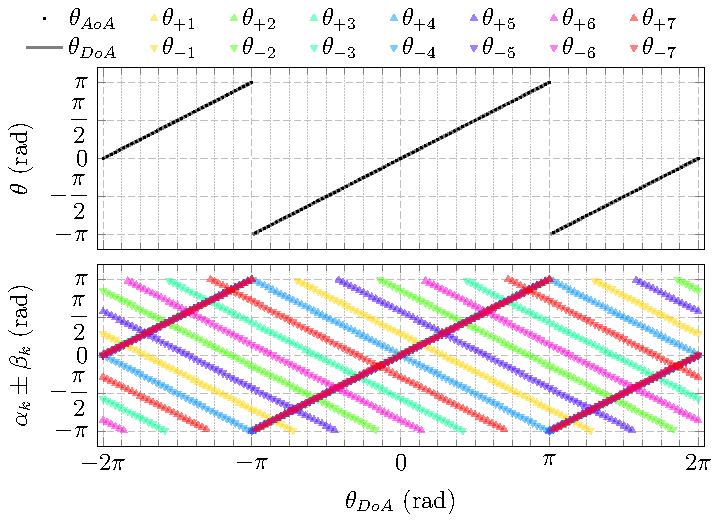
\includegraphics[height=0.785\textheight]{../pictures/simul_POLY_7_R_50.pdf}
			\caption*{\tiny Fonte: Autor, saída gráfica disponível em \href{https://github.com/HeckRodSav/TG/blob/main/documentation/pictures/POLY_7/simul_POLY_7_R_50.gif}{\underline{GitHub}}.}
		\end{figure}
	\end{frame}
	\begin{frame}
		\begin{figure}
			\centering
			\caption*{Caso $\text{SNR} = \SI{0}{\deci\bel}$, sem atenuação.}
			% \begin{tikzpicture}
    % \pgfsetfillopacity{0.5}

    \def\fileName{simul_POLY_7_R_50_SNR_1}
    % \def\fileAddress{../../code/simul/Output/POLY_7/\fileName.dat}
    \def\fileAddress{../data/POLY_7/\fileName.dat}
    % \def\fileAddress{../data/\fileName.dat}

    \def\height{.225\linewidth}
    \def\width{0.75\linewidth}
    \def\distance{0.25cm}
    \def\xmin{-1}
    \def\xmax{101}

    \begin{axis} %configuração do eixo Y esquerdo e eixo X
    [
        name=plot1,
        reverse legend, % inverte a ordem que os items aparecem na legenda
    	% legend style={
        % 	at=(current bounding box.north),
        % 	anchor=south,
        % 	legend columns=6,
        % 	transpose legend,
        % 	draw=none,
        % 	/tikz/every even column/.append style={column sep=0.5cm}
    	% }, % onde exibir
        % axis x line=center,
        % axis y line=center,
        height=\height, % altura da região do gráfico
        width=\width, % largura da região do gráfico
        scale only axis, %
        minor grid style={densely dotted}, % estilo da grade secundária
        major grid style={densely dashed}, % estilo da grade principal
        grid style={lightgray, thin}, % cor das grades
        % axis on top, % forçar grade para ficar por cima do gráfico
        %
        %
        % axis y line*=left, % define gráfico para usar eixo esquerdo sem exibir direito
        y tick label style={
            /pgf/number format/.cd,
            fixed,
            % fixed zerofill,
            precision=1, % quantidade de casas depois da virgula
            /tikz/.cd
        },
        % y filter/.expression={y==0 ? NaN : y},
        scaled y ticks = false,
        ylabel={$\alpha_{k}\pm \beta_{k}$ (\si{\radian})}, % titulo eixo vertical
        % yticklabel={\pgfmathparse{\tick-50}\pgfmathprintnumber{\pgfmathresult}}, % fator multiplicativo para valores do eixo
        y tick label style={/pgf/number format/1000 sep=}, % Altera marcação de milhar
        % yticklabel style={rotate=90},
		ytick={-3.1415, -1.5708, 0, 1.5708, 3.1415},
		yticklabels={$-\pi$,$-\dfrac{\pi}{2}$,$0$,$\dfrac{\pi}{2}$,$\pi$},
        % ytick={0,1,2,3,4,5}, % lista de valores a serem utilizados no eixo
        % ymin=-1,  ymax=4,  % intervalo de valores no eixo y -> na dúvida, deixe comentado
        %
        ymajorgrids=true, % exibir grade principal y
        yminorgrids=true, % exibir grade secundária y
        minor y tick num=4, % contagem de linhas na grade secundária y
        % ybar,
        %
        %
        xlabel={$\theta_{DoA}$ (\si{\radian})}, % título eixo horizontal
        % xticklabel={\pgfmathparse{\tick-50}\pgfmathprintnumber{\pgfmathresult}}, % fator multiplicativo para valores do eixo
        % xticklabels={}, % fator multiplicativo para valores do eixo
		% xtick={0, 12.5, 25, 37.5, 50, 62.6, 75, 87.5, 100},
		% xticklabels={$-2~\pi$,$-\dfrac{3~\pi}{2}$,$-\pi$,$-\dfrac{\pi}{2}$,$0$,$-\dfrac{\pi}{2}$,$\pi$,$-\dfrac{3~\pi}{2}$,$2~\pi$},
		xtick={0, 25, 50, 75, 100},
		xticklabels={$-2 \pi$,$-\pi$,$0$,$\pi$,$2 \pi$},
        % xmode=log,
        % log ticks with fixed point,
        % x filter/.code=\pgfmathparse{#1 + 6.90775527898214},
        x tick label style={
            /pgf/number format/.cd,
            fixed,
            % fixed zerofill,
            precision=1,
            /tikz/.cd,
            /pgf/number format/use comma
        },
        xmin=\xmin, xmax=\xmax, % intervalo de valores no eixo x -> na dúvida, deixe comentado
        scaled x ticks = false,
        %
        xmajorgrids=true, % exibir grade principal x
        xminorgrids=true, % exibir grade secundária x
        minor x tick num=7, % contagem de linhas na grade secundária x
        %
        %
        %
        % unbounded coords=jump,
        % jump threshold/.initial=0.25
    ]

	\addplot[
        antena_7_1,
        mark=triangle*,
		opacity=0.5,
        only marks,
        % smooth
    ] table [
        % col sep=comma,
        x=percent, % cabeçalho da coluna de dados X no arquivo
        y=delta_1_x_7, % cabeçalho da coluna de dados Y no arquivo
    ]
    {\fileAddress};	\label{\fileName.1.1}

    \addplot[
        antena_7_1,
        mark=triangle*,
		opacity=0.5,
		mark options={rotate=180},
        only marks,
        % smooth
    ] table [
        % col sep=comma,
        x=percent, % cabeçalho da coluna de dados X no arquivo
        y=delta_7_x_1, % cabeçalho da coluna de dados Y no arquivo
    ]
    {\fileAddress};	\label{\fileName.1.2}

	\addplot[
        antena_7_2,
        mark=triangle*,
		opacity=0.5,
        only marks,
        % smooth
    ] table [
        % col sep=comma,
        x=percent, % cabeçalho da coluna de dados X no arquivo
        y=delta_2_x_1, % cabeçalho da coluna de dados Y no arquivo
    ]
    {\fileAddress};	\label{\fileName.1.3}

    \addplot[
        antena_7_2,
        mark=triangle*,
		opacity=0.5,
		mark options={rotate=180},
        only marks,
        % smooth
    ] table [
        % col sep=comma,
        x=percent, % cabeçalho da coluna de dados X no arquivo
        y=delta_1_x_2, % cabeçalho da coluna de dados Y no arquivo
    ]
    {\fileAddress};	\label{\fileName.1.4}

	\addplot[
        antena_7_3,
        mark=triangle*,
		opacity=0.5,
        only marks,
        % smooth
    ] table [
        % col sep=comma,
        x=percent, % cabeçalho da coluna de dados X no arquivo
        y=delta_3_x_2, % cabeçalho da coluna de dados Y no arquivo
    ]
    {\fileAddress};	\label{\fileName.1.5}

    \addplot[
        antena_7_3,
        mark=triangle*,
		opacity=0.5,
		mark options={rotate=180},
        only marks,
        % smooth
    ] table [
        % col sep=comma,
        x=percent, % cabeçalho da coluna de dados X no arquivo
        y=delta_2_x_3, % cabeçalho da coluna de dados Y no arquivo
    ]
    {\fileAddress};	\label{\fileName.1.6}

	\addplot[
        antena_7_4,
        mark=triangle*,
		opacity=0.5,
        only marks,
        % smooth
    ] table [
        % col sep=comma,
        x=percent, % cabeçalho da coluna de dados X no arquivo
        y=delta_4_x_3, % cabeçalho da coluna de dados Y no arquivo
    ]
    {\fileAddress};	\label{\fileName.1.7}

    \addplot[
        antena_7_4,
        mark=triangle*,
		opacity=0.5,
		mark options={rotate=180},
        only marks,
        % smooth
    ] table [
        % col sep=comma,
        x=percent, % cabeçalho da coluna de dados X no arquivo
        y=delta_3_x_4, % cabeçalho da coluna de dados Y no arquivo
    ]
    {\fileAddress};	\label{\fileName.1.8}

	\addplot[
        antena_7_5,
        mark=triangle*,
		opacity=0.5,
        only marks,
        % smooth
    ] table [
        % col sep=comma,
        x=percent, % cabeçalho da coluna de dados X no arquivo
        y=delta_5_x_4, % cabeçalho da coluna de dados Y no arquivo
    ]
    {\fileAddress};	\label{\fileName.1.9}

    \addplot[
        antena_7_5,
        mark=triangle*,
		opacity=0.5,
		mark options={rotate=180},
        only marks,
        % smooth
    ] table [
        % col sep=comma,
        x=percent, % cabeçalho da coluna de dados X no arquivo
        y=delta_4_x_5, % cabeçalho da coluna de dados Y no arquivo
    ]
    {\fileAddress};	\label{\fileName.1.10}

	\addplot[
        antena_7_6,
        mark=triangle*,
		opacity=0.5,
        only marks,
        % smooth
    ] table [
        % col sep=comma,
        x=percent, % cabeçalho da coluna de dados X no arquivo
        y=delta_6_x_5, % cabeçalho da coluna de dados Y no arquivo
    ]
    {\fileAddress};	\label{\fileName.1.11}

    \addplot[
        antena_7_6,
        mark=triangle*,
		opacity=0.5,
		mark options={rotate=180},
        only marks,
        % smooth
    ] table [
        % col sep=comma,
        x=percent, % cabeçalho da coluna de dados X no arquivo
        y=delta_5_x_6 % cabeçalho da coluna de dados Y no arquivo
    ]
    {\fileAddress};	\label{\fileName.1.12}

	\addplot[
        antena_7_7,
        mark=triangle*,
		opacity=0.5,
        only marks,
        % smooth
    ] table [
        % col sep=comma,
        x=percent, % cabeçalho da coluna de dados X no arquivo
        y=delta_7_x_6, % cabeçalho da coluna de dados Y no arquivo
    ]
    {\fileAddress};	\label{\fileName.1.13}

    \addplot[
        antena_7_7,
        mark=triangle*,
		opacity=0.5,
		mark options={rotate=180},
        only marks,
        % smooth
    ] table [
        % col sep=comma,
        x=percent, % cabeçalho da coluna de dados X no arquivo
        y=delta_6_x_7, % cabeçalho da coluna de dados Y no arquivo
    ]
    {\fileAddress};	\label{\fileName.1.14}

    \end{axis}

    % \begin{axis} %configuração do eixo Y direito e legenda
    % [
    %     legend cell align=left, % alinhamento de texto na legenda
    %     % legend pos={outer north east}, % onde exibir caixa de legenda
    %     % reverse legend, % inverte a ordem que os items aparecem na legenda
    % 	legend style={
    %     	at=(current bounding box.north),
    %     	anchor=south,
    %     	legend columns=2,
    %     % 	transpose legend,
    %     	draw=none
    % 	}, % onde exibir
    %     % axis x line=center,
    %     % axis y line=center,
    %     height=\height, % altura da região do gráfico
    %     width=\width, % largura da região do gráfico
    %     scale only axis, %
    %     minor grid style={densely dotted}, % estilo da grade secundária
    %     major grid style={densely dashed}, % estilo da grade principal
    %     grid style={lightgray, thin}, % cor das grades
    %     % axis on top, % forçar grade para ficar por cima do gráfico
    %     %
    %     %
    %     axis y line*=right, % define gráfico para usar eixo direito sem exibir esquerdo
    %     ylabel={$V_{out}$ (\si{\milli\volt})}, % titulo eixo vertical
    %     y tick label style={
    %         /pgf/number format/.cd,
    %         fixed,
    %         % fixed zerofill,
    %         precision=3, % quantidade de casas depois da virgula
    %         /tikz/.cd,
    %         /pgf/number format/use comma
    %     },
    %     % y filter/.expression={y==0 ? NaN : y},
    %     scaled y ticks = false,
    %     % yticklabel={\pgfmathparse{\tick*10^3}\pgfmathprintnumber{\pgfmathresult}}, % fator multiplicativo para valores do eixo
    %     y tick label style={/pgf/number format/1000 sep=}, % Altera marcação de milhar
    %     % yticklabel style={rotate=90},
    %     % ytick={-12,-6,0,6,12}, % lista de valores a serem utilizados no eixo
    %     % ymin=0.76503, ymax=0.76509,  % intervalo de valores no eixo y -> na dúvida, deixe comentado
    %     %
    %     ymajorgrids=false, % exibir grade principal y
    %     yminorgrids=false, % exibir grade secundária y
    %     minor y tick num=4, % contagem de linhas na grade secundária y
    %     % ybar,
    %     %
    %     %
    %     axis x line=none, %oculta eixo inferior quando o gráfico anterior já exibe
    %     % xlabel={Frequência (\si{\hertz})}, % título eixo horizontal
    %     % xticklabel={\pgfmathparse{\tick*10^3}\pgfmathprintnumber{\pgfmathresult}}, % fator multiplicativo para valores do eixo
    %     % xmode=log,
    %     % log ticks with fixed point,
    %     % x filter/.code=\pgfmathparse{#1 + 6.90775527898214},
    %     % x tick label style={
    %     %     /pgf/number format/.cd,
    %     %     fixed,
    %     %     % fixed zerofill,
    %     %     precision=0,
    %     %     /tikz/.cd,
    %     %     /pgf/number format/use comma
    %     % },
    %     xmin=\xmin, xmax=\xmax, % intervalo de valores no eixo x -> na dúvida, deixe comentado
    %     % scaled x ticks = true,
    %     %
    %     % xmajorgrids=true, % exibir grade principal x
    %     % xminorgrids=true, % exibir grade secundária x
    %     % minor x tick num=7, % contagem de linhas na grade secundária x
    %     %
    %     %
    %     %
    % ]



    % \addplot[mark=none,red, thick]
    % table [
    %     x=time, % cabeçalho da coluna de dados X no arquivo
    %     y=vout % cabeçalho da coluna de dados Y no arquivo
    % ]
    % {graficos/dados/booster.dat};  \label{\fileName.1.2}

    % % \addlegendimage{/pgfplots/refstyle=_1_2}

    % % \addplot[ForestGreen, densely dashdotted, thick]
    % % coordinates
    % % {
    % %     (\pgfkeysvalueof{/pgfplots/xmin},12)
    % %     (\pgfkeysvalueof{/pgfplots/xmax},12)
    % % };
    % % % \addlegendentry{$V_{out}=\pm\SI{12}{\volt}$}

    % % \addplot[ForestGreen, densely dashdotted, thick]
    % % coordinates
    % % {
    % %     (\pgfkeysvalueof{/pgfplots/xmin},-12)
    % %     (\pgfkeysvalueof{/pgfplots/xmax},-12)
    % % };

    % \end{axis}

    \begin{axis} %configuração do eixo Y esquerdo e eixo X
    [
        at={($(plot1.north)+(0,\distance)$)},
        anchor=south,
        % reverse legend, % inverte a ordem que os items aparecem na legenda
		legend style={
        	at=(current bounding box.north),
        	anchor=south,
        	legend columns=2,
        	transpose legend,
        	draw=none,
        	/tikz/every even column/.append style={column sep=0.5cm}
    	}, % onde exibir
        samples=505,
        domain=0:100,
        % axis x line=center,
        % axis y line=center,
        height=\height, % altura da região do gráfico
        width=\width, % largura da região do gráfico
        scale only axis, %
        minor grid style={densely dotted}, % estilo da grade secundária
        major grid style={densely dashed}, % estilo da grade principal
        grid style={lightgray, thin}, % cor das grades
        % axis on top, % forçar grade para ficar por cima do gráfico
        %
        %
        % axis y line*=left, % define gráfico para usar eixo esquerdo sem exibir direito
        y tick label style={
            /pgf/number format/.cd,
            fixed,
            % fixed zerofill,
            precision=1, % quantidade de casas depois da virgula
            /tikz/.cd
        },
        % y filter/.expression={y==0 ? NaN : y},
        scaled y ticks = false,
        ylabel={$\theta$ (\si{\radian})}, % titulo eixo vertical
        % yticklabel={\pgfmathparse{\tick*10^3}\pgfmathprintnumber{\pgfmathresult}}, % fator multiplicativo para valores do eixo
        y tick label style={/pgf/number format/1000 sep=}, % Altera marcação de milhar
        % yticklabel style={rotate=90},
		ytick={-3.1415, -1.5708, 0, 1.5708, 3.1415},
		yticklabels={$-\pi$,$-\dfrac{\pi}{2}$,$0$,$\dfrac{\pi}{2}$,$\pi$},
        % ytick={0,1,2,3,4,5}, % lista de valores a serem utilizados no eixo
        % ymin=-1,  ymax=4,  % intervalo de valores no eixo y -> na dúvida, deixe comentado
        %
        ymajorgrids=true, % exibir grade principal y
        yminorgrids=true, % exibir grade secundária y
        minor y tick num=4, % contagem de linhas na grade secundária y
        % ybar,
        %
        %
        % xlabel={Tempo (\si{\milli\second})}, % título eixo horizontal
        % xticklabel={\pgfmathparse{\tick*10^3}\pgfmathprintnumber{\pgfmathresult}}, % fator multiplicativo para valores do eixo
		xtick={0, 25, 50, 75, 100},
        xticklabels={}, % fator multiplicativo para valores do eixo
        % xmode=log,
        % log ticks with fixed point,
        % x filter/.code=\pgfmathparse{#1 + 6.90775527898214},
        x tick label style={
            /pgf/number format/.cd,
            fixed,
            % fixed zerofill,
            precision=1,
            /tikz/.cd,
            /pgf/number format/use comma
        },
        xmin=\xmin, xmax=\xmax, % intervalo de valores no eixo x -> na dúvida, deixe comentado
        scaled x ticks = false,
        %
        xmajorgrids=true, % exibir grade principal x
        xminorgrids=true, % exibir grade secundária x
        minor x tick num=7, % contagem de linhas na grade secundária x
        %
        %
        %
        unbounded coords=jump,
		jump threshold/.initial=0.01
    ]


    \addplot[
        Black,
        mark=*,
		mark size=0.5pt,
        only marks,
        % smooth
    ] table [
        % col sep=comma,
        x=percent, % cabeçalho da coluna de dados X no arquivo
        y=choose_angle, % cabeçalho da coluna de dados Y no arquivo
	]
	{\fileAddress};	\addlegendentry{$\theta_{AoA}$}

	% \addplot[
	% 	Black,
	% 	mark=o,
	% 	mark size=1.5pt,
	% 	only marks,
	% 	opacity=0.5,
    %     thick,
	% 	% smooth
	% ] table [
	% 	% col sep=comma,
	% 	x=percent, % cabeçalho da coluna de dados X no arquivo
	% 	y=ang_W, % cabeçalho da coluna de dados Y no arquivo
	% ]
	% {\fileAddress};
    \addplot [
        Black,
        opacity=0.5,
        mark=none,
        mark size=5pt,
        very thick,
        % only marks,
        % smooth
    ] {((x==25)||(x==75)?nan:pi*(mod(x+25,50)-25)/25)};
    \addlegendentry{$\theta_{DoA}$}


	\addlegendimage{/pgfplots/refstyle=\fileName.1.1}\addlegendentry{$\theta_{+1}$}
	\addlegendimage{/pgfplots/refstyle=\fileName.1.2}\addlegendentry{$\theta_{-1}$}

	\addlegendimage{/pgfplots/refstyle=\fileName.1.3}\addlegendentry{$\theta_{+2}$}
	\addlegendimage{/pgfplots/refstyle=\fileName.1.4}\addlegendentry{$\theta_{-2}$}

    \addlegendimage{/pgfplots/refstyle=\fileName.1.5}\addlegendentry{$\theta_{+3}$}
	\addlegendimage{/pgfplots/refstyle=\fileName.1.6}\addlegendentry{$\theta_{-3}$}

    \addlegendimage{/pgfplots/refstyle=\fileName.1.7}\addlegendentry{$\theta_{+4}$}
	\addlegendimage{/pgfplots/refstyle=\fileName.1.8}\addlegendentry{$\theta_{-4}$}

    \addlegendimage{/pgfplots/refstyle=\fileName.1.9}\addlegendentry{$\theta_{+5}$}
	\addlegendimage{/pgfplots/refstyle=\fileName.1.10}\addlegendentry{$\theta_{-5}$}

    \addlegendimage{/pgfplots/refstyle=\fileName.1.11}\addlegendentry{$\theta_{+6}$}
	\addlegendimage{/pgfplots/refstyle=\fileName.1.12}\addlegendentry{$\theta_{-6}$}

    \addlegendimage{/pgfplots/refstyle=\fileName.1.13}\addlegendentry{$\theta_{+7}$}
	\addlegendimage{/pgfplots/refstyle=\fileName.1.14}\addlegendentry{$\theta_{-7}$}


    \end{axis}

    % \begin{axis} %configuração do eixo Y direito e legenda
    % [
    %     at={($(plot1.north)+(0,\distance)$)},
    %     anchor=south,
    %     legend cell align=left, % alinhamento de texto na legenda
    %     % legend pos={outer north east}, % onde exibir caixa de legenda
    %     % reverse legend, % inverte a ordem que os items aparecem na legenda
    % 	legend style={
    %     	at=(current bounding box.north),
    %     	anchor=south,
    %     	legend columns=3,
    %     % 	transpose legend,
    %     	draw=none,
    %     	/tikz/every even column/.append style={column sep=0.5cm}
    % 	}, % onde exibir
    %     % axis x line=center,
    %     % axis y line=center,
    %     height=\height, % altura da região do gráfico
    %     width=\width, % largura da região do gráfico
    %     scale only axis, %
    %     minor grid style={densely dotted}, % estilo da grade secundária
    %     major grid style={densely dashed}, % estilo da grade principal
    %     grid style={lightgray, thin}, % cor das grades
    %     % axis on top, % forçar grade para ficar por cima do gráfico
    %     %
    %     %
    %     axis y line*=right, % define gráfico para usar eixo direito sem exibir esquerdo
    %     ylabel={$V_{out}$ (\si{\volt})}, % titulo eixo vertical
    %     y tick label style={
    %         /pgf/number format/.cd,
    %         fixed,
    %         % fixed zerofill,
    %         precision=3, % quantidade de casas depois da virgula
    %         /tikz/.cd,
    %         /pgf/number format/use comma
    %     },
    %     % y filter/.expression={y==0 ? NaN : y},
    %     scaled y ticks = false,
    %     % yticklabel={\pgfmathparse{\tick*10^3}\pgfmathprintnumber{\pgfmathresult}}, % fator multiplicativo para valores do eixo
    %     y tick label style={/pgf/number format/1000 sep=}, % Altera marcação de milhar
    %     % yticklabel style={rotate=90},
    %     % ytick={-12,-6,0,6,12}, % lista de valores a serem utilizados no eixo
    %     % ymin=0.76503, ymax=0.76509,  % intervalo de valores no eixo y -> na dúvida, deixe comentado
    %     %
    %     ymajorgrids=false, % exibir grade principal y
    %     yminorgrids=false, % exibir grade secundária y
    %     minor y tick num=4, % contagem de linhas na grade secundária y
    %     % ybar,
    %     %
    %     %
    %     axis x line=none, %oculta eixo inferior quando o gráfico anterior já exibe
    %     % xlabel={Frequência (\si{\hertz})}, % título eixo horizontal
    %     % xticklabel={\pgfmathparse{\tick*10^3}\pgfmathprintnumber{\pgfmathresult}}, % fator multiplicativo para valores do eixo
    %     % xmode=log,
    %     % log ticks with fixed point,
    %     % x filter/.code=\pgfmathparse{#1 + 6.90775527898214},
    %     % x tick label style={
    %     %     /pgf/number format/.cd,
    %     %     fixed,
    %     %     % fixed zerofill,
    %     %     precision=0,
    %     %     /tikz/.cd,
    %     %     /pgf/number format/use comma
    %     % },
    %     xmin=\xmin, xmax=\xmax, % intervalo de valores no eixo x -> na dúvida, deixe comentado
    %     % scaled x ticks = true,
    %     %
    %     % xmajorgrids=true, % exibir grade principal x
    %     % xminorgrids=true, % exibir grade secundária x
    %     % minor x tick num=10, % contagem de linhas na grade secundária x
    %     %
    %     %
    %     %
    % ]


    % \addlegendimage{/pgfplots/refstyle=_2_1}\addlegendentry{$V_{in}$}
    % \addlegendimage{/pgfplots/refstyle=_2_2}\addlegendentry{$V_{in}$}
    % % \addplot[mark=none,red, thick]
    % % table [
    % %     x=time, % cabeçalho da coluna de dados X no arquivo
    % %     y=vout % cabeçalho da coluna de dados Y no arquivo
    % % ]
    % % {graficos/dados/booster.dat}; % \label{\fileName.1.2}
    % % \addlegendentry{$V_{out}$}

    % \addlegendimage{/pgfplots/refstyle=_1_1}\addlegendentry{$I_{out}$}
    % \addlegendimage{/pgfplots/refstyle=_1_2}\addlegendentry{$I_{out}$}

    % % \addlegendimage{/pgfplots/refstyle=_1_2}

    % % \addplot[ForestGreen, densely dashdotted, thick]
    % % coordinates
    % % {
    % %     (\pgfkeysvalueof{/pgfplots/xmin},12)
    % %     (\pgfkeysvalueof{/pgfplots/xmax},12)
    % % };
    % % % \addlegendentry{$V_{out}=\pm\SI{12}{\volt}$}

    % % \addplot[ForestGreen, densely dashdotted, thick]
    % % coordinates
    % % {
    % %     (\pgfkeysvalueof{/pgfplots/xmin},-12)
    % %     (\pgfkeysvalueof{/pgfplots/xmax},-12)
    % % };

    % \end{axis}



\end{tikzpicture}

			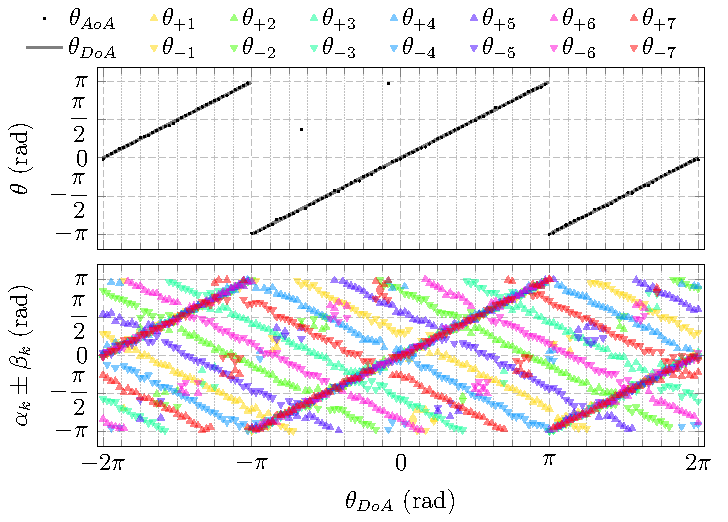
\includegraphics[height=0.785\textheight]{../pictures/simul_POLY_7_R_50_SNR_1.pdf}
			\caption*{\tiny Fonte: Autor, saída gráfica disponível em \href{https://github.com/HeckRodSav/TG/blob/main/documentation/pictures/POLY_7/simul_POLY_7_R_50_SNR_1.gif}{\underline{GitHub}}.}
		\end{figure}
	\end{frame}
	\begin{frame}
		\begin{figure}
			\centering
			\caption*{Caso $\text{SNR} = \SI{0}{\deci\bel}$, com atenuação.}
			% \begin{tikzpicture}
    % \pgfsetfillopacity{0.5}

    \def\fileName{simul_POLY_7_R_50_SNR_1_ATT}
    % \def\fileAddress{../../code/simul/Output/POLY_7/\fileName.dat}
    \def\fileAddress{../data/POLY_7/\fileName.dat}
    % \def\fileAddress{../data/\fileName.dat}

    \def\height{.225\linewidth}
    \def\width{0.75\linewidth}
    \def\distance{0.25cm}
    \def\xmin{-1}
    \def\xmax{101}

    \begin{axis} %configuração do eixo Y esquerdo e eixo X
    [
        name=plot1,
        reverse legend, % inverte a ordem que os items aparecem na legenda
    	% legend style={
        % 	at=(current bounding box.north),
        % 	anchor=south,
        % 	legend columns=6,
        % 	transpose legend,
        % 	draw=none,
        % 	/tikz/every even column/.append style={column sep=0.5cm}
    	% }, % onde exibir
        % axis x line=center,
        % axis y line=center,
        height=\height, % altura da região do gráfico
        width=\width, % largura da região do gráfico
        scale only axis, %
        minor grid style={densely dotted}, % estilo da grade secundária
        major grid style={densely dashed}, % estilo da grade principal
        grid style={lightgray, thin}, % cor das grades
        % axis on top, % forçar grade para ficar por cima do gráfico
        %
        %
        % axis y line*=left, % define gráfico para usar eixo esquerdo sem exibir direito
        y tick label style={
            /pgf/number format/.cd,
            fixed,
            % fixed zerofill,
            precision=1, % quantidade de casas depois da virgula
            /tikz/.cd
        },
        % y filter/.expression={y==0 ? NaN : y},
        scaled y ticks = false,
        ylabel={$\alpha_{k}\pm \beta_{k}$ (\si{\radian})}, % titulo eixo vertical
        % yticklabel={\pgfmathparse{\tick-50}\pgfmathprintnumber{\pgfmathresult}}, % fator multiplicativo para valores do eixo
        y tick label style={/pgf/number format/1000 sep=}, % Altera marcação de milhar
        % yticklabel style={rotate=90},
		ytick={-3.1415, -1.5708, 0, 1.5708, 3.1415},
		yticklabels={$-\pi$,$-\dfrac{\pi}{2}$,$0$,$\dfrac{\pi}{2}$,$\pi$},
        % ytick={0,1,2,3,4,5}, % lista de valores a serem utilizados no eixo
        % ymin=-1,  ymax=4,  % intervalo de valores no eixo y -> na dúvida, deixe comentado
        %
        ymajorgrids=true, % exibir grade principal y
        yminorgrids=true, % exibir grade secundária y
        minor y tick num=4, % contagem de linhas na grade secundária y
        % ybar,
        %
        %
        xlabel={$\theta_{DoA}$ (\si{\radian})}, % título eixo horizontal
        % xticklabel={\pgfmathparse{\tick-50}\pgfmathprintnumber{\pgfmathresult}}, % fator multiplicativo para valores do eixo
        % xticklabels={}, % fator multiplicativo para valores do eixo
		% xtick={0, 12.5, 25, 37.5, 50, 62.6, 75, 87.5, 100},
		% xticklabels={$-2~\pi$,$-\dfrac{3~\pi}{2}$,$-\pi$,$-\dfrac{\pi}{2}$,$0$,$-\dfrac{\pi}{2}$,$\pi$,$-\dfrac{3~\pi}{2}$,$2~\pi$},
		xtick={0, 25, 50, 75, 100},
		xticklabels={$-2 \pi$,$-\pi$,$0$,$\pi$,$2 \pi$},
        % xmode=log,
        % log ticks with fixed point,
        % x filter/.code=\pgfmathparse{#1 + 6.90775527898214},
        x tick label style={
            /pgf/number format/.cd,
            fixed,
            % fixed zerofill,
            precision=1,
            /tikz/.cd,
            /pgf/number format/use comma
        },
        xmin=\xmin, xmax=\xmax, % intervalo de valores no eixo x -> na dúvida, deixe comentado
        scaled x ticks = false,
        %
        xmajorgrids=true, % exibir grade principal x
        xminorgrids=true, % exibir grade secundária x
        minor x tick num=7, % contagem de linhas na grade secundária x
        %
        %
        %
        % unbounded coords=jump,
        % jump threshold/.initial=0.25
    ]

	\addplot[
        cmyk_G,
        mark=triangle*,
		opacity=0.5,
        only marks,
        % smooth
    ] table [
        % col sep=comma,
        x=percent, % cabeçalho da coluna de dados X no arquivo
        y=delta_1_x_7, % cabeçalho da coluna de dados Y no arquivo
    ]
    {\fileAddress};	\label{\fileName.1.1}

    \addplot[
        cmyk_G,
        mark=triangle*,
		opacity=0.5,
		mark options={rotate=180},
        only marks,
        % smooth
    ] table [
        % col sep=comma,
        x=percent, % cabeçalho da coluna de dados X no arquivo
        y=delta_7_x_1, % cabeçalho da coluna de dados Y no arquivo
    ]
    {\fileAddress};	\label{\fileName.1.2}

	\addplot[
        cmyk_B,
        mark=triangle*,
		opacity=0.5,
        only marks,
        % smooth
    ] table [
        % col sep=comma,
        x=percent, % cabeçalho da coluna de dados X no arquivo
        y=delta_2_x_1, % cabeçalho da coluna de dados Y no arquivo
    ]
    {\fileAddress};	\label{\fileName.1.3}

    \addplot[
        cmyk_B,
        mark=triangle*,
		opacity=0.5,
		mark options={rotate=180},
        only marks,
        % smooth
    ] table [
        % col sep=comma,
        x=percent, % cabeçalho da coluna de dados X no arquivo
        y=delta_1_x_2, % cabeçalho da coluna de dados Y no arquivo
    ]
    {\fileAddress};	\label{\fileName.1.4}

	\addplot[
        cmyk_R,
        mark=triangle*,
		opacity=0.5,
        only marks,
        % smooth
    ] table [
        % col sep=comma,
        x=percent, % cabeçalho da coluna de dados X no arquivo
        y=delta_3_x_2, % cabeçalho da coluna de dados Y no arquivo
    ]
    {\fileAddress};	\label{\fileName.1.5}

    \addplot[
        cmyk_R,
        mark=triangle*,
		opacity=0.5,
		mark options={rotate=180},
        only marks,
        % smooth
    ] table [
        % col sep=comma,
        x=percent, % cabeçalho da coluna de dados X no arquivo
        y=delta_2_x_3, % cabeçalho da coluna de dados Y no arquivo
    ]
    {\fileAddress};	\label{\fileName.1.6}

	\addplot[
        cmyk_C,
        mark=triangle*,
		opacity=0.5,
        only marks,
        % smooth
    ] table [
        % col sep=comma,
        x=percent, % cabeçalho da coluna de dados X no arquivo
        y=delta_4_x_3, % cabeçalho da coluna de dados Y no arquivo
    ]
    {\fileAddress};	\label{\fileName.1.7}

    \addplot[
        cmyk_C,
        mark=triangle*,
		opacity=0.5,
		mark options={rotate=180},
        only marks,
        % smooth
    ] table [
        % col sep=comma,
        x=percent, % cabeçalho da coluna de dados X no arquivo
        y=delta_3_x_4, % cabeçalho da coluna de dados Y no arquivo
    ]
    {\fileAddress};	\label{\fileName.1.8}

	\addplot[
        Goldenrod,
        mark=triangle*,
		opacity=0.5,
        only marks,
        % smooth
    ] table [
        % col sep=comma,
        x=percent, % cabeçalho da coluna de dados X no arquivo
        y=delta_5_x_4, % cabeçalho da coluna de dados Y no arquivo
    ]
    {\fileAddress};	\label{\fileName.1.9}

    \addplot[
        Goldenrod,
        mark=triangle*,
		opacity=0.5,
		mark options={rotate=180},
        only marks,
        % smooth
    ] table [
        % col sep=comma,
        x=percent, % cabeçalho da coluna de dados X no arquivo
        y=delta_4_x_5, % cabeçalho da coluna de dados Y no arquivo
    ]
    {\fileAddress};	\label{\fileName.1.10}

	\addplot[
        DeepPink,
        mark=triangle*,
		opacity=0.5,
        only marks,
        % smooth
    ] table [
        % col sep=comma,
        x=percent, % cabeçalho da coluna de dados X no arquivo
        y=delta_6_x_5, % cabeçalho da coluna de dados Y no arquivo
    ]
    {\fileAddress};	\label{\fileName.1.11}

    \addplot[
        DeepPink,
        mark=triangle*,
		opacity=0.5,
		mark options={rotate=180},
        only marks,
        % smooth
    ] table [
        % col sep=comma,
        x=percent, % cabeçalho da coluna de dados X no arquivo
        y=delta_5_x_6 % cabeçalho da coluna de dados Y no arquivo
    ]
    {\fileAddress};	\label{\fileName.1.12}

	\addplot[
        Sienna,
        mark=triangle*,
		opacity=0.5,
        only marks,
        % smooth
    ] table [
        % col sep=comma,
        x=percent, % cabeçalho da coluna de dados X no arquivo
        y=delta_7_x_6, % cabeçalho da coluna de dados Y no arquivo
    ]
    {\fileAddress};	\label{\fileName.1.13}

    \addplot[
        Sienna,
        mark=triangle*,
		opacity=0.5,
		mark options={rotate=180},
        only marks,
        % smooth
    ] table [
        % col sep=comma,
        x=percent, % cabeçalho da coluna de dados X no arquivo
        y=delta_6_x_7, % cabeçalho da coluna de dados Y no arquivo
    ]
    {\fileAddress};	\label{\fileName.1.14}

    \end{axis}

    % \begin{axis} %configuração do eixo Y direito e legenda
    % [
    %     legend cell align=left, % alinhamento de texto na legenda
    %     % legend pos={outer north east}, % onde exibir caixa de legenda
    %     % reverse legend, % inverte a ordem que os items aparecem na legenda
    % 	legend style={
    %     	at=(current bounding box.north),
    %     	anchor=south,
    %     	legend columns=2,
    %     % 	transpose legend,
    %     	draw=none
    % 	}, % onde exibir
    %     % axis x line=center,
    %     % axis y line=center,
    %     height=\height, % altura da região do gráfico
    %     width=\width, % largura da região do gráfico
    %     scale only axis, %
    %     minor grid style={densely dotted}, % estilo da grade secundária
    %     major grid style={densely dashed}, % estilo da grade principal
    %     grid style={lightgray, thin}, % cor das grades
    %     % axis on top, % forçar grade para ficar por cima do gráfico
    %     %
    %     %
    %     axis y line*=right, % define gráfico para usar eixo direito sem exibir esquerdo
    %     ylabel={$V_{out}$ (\si{\milli\volt})}, % titulo eixo vertical
    %     y tick label style={
    %         /pgf/number format/.cd,
    %         fixed,
    %         % fixed zerofill,
    %         precision=3, % quantidade de casas depois da virgula
    %         /tikz/.cd,
    %         /pgf/number format/use comma
    %     },
    %     % y filter/.expression={y==0 ? NaN : y},
    %     scaled y ticks = false,
    %     % yticklabel={\pgfmathparse{\tick*10^3}\pgfmathprintnumber{\pgfmathresult}}, % fator multiplicativo para valores do eixo
    %     y tick label style={/pgf/number format/1000 sep=}, % Altera marcação de milhar
    %     % yticklabel style={rotate=90},
    %     % ytick={-12,-6,0,6,12}, % lista de valores a serem utilizados no eixo
    %     % ymin=0.76503, ymax=0.76509,  % intervalo de valores no eixo y -> na dúvida, deixe comentado
    %     %
    %     ymajorgrids=false, % exibir grade principal y
    %     yminorgrids=false, % exibir grade secundária y
    %     minor y tick num=4, % contagem de linhas na grade secundária y
    %     % ybar,
    %     %
    %     %
    %     axis x line=none, %oculta eixo inferior quando o gráfico anterior já exibe
    %     % xlabel={Frequência (\si{\hertz})}, % título eixo horizontal
    %     % xticklabel={\pgfmathparse{\tick*10^3}\pgfmathprintnumber{\pgfmathresult}}, % fator multiplicativo para valores do eixo
    %     % xmode=log,
    %     % log ticks with fixed point,
    %     % x filter/.code=\pgfmathparse{#1 + 6.90775527898214},
    %     % x tick label style={
    %     %     /pgf/number format/.cd,
    %     %     fixed,
    %     %     % fixed zerofill,
    %     %     precision=0,
    %     %     /tikz/.cd,
    %     %     /pgf/number format/use comma
    %     % },
    %     xmin=\xmin, xmax=\xmax, % intervalo de valores no eixo x -> na dúvida, deixe comentado
    %     % scaled x ticks = true,
    %     %
    %     % xmajorgrids=true, % exibir grade principal x
    %     % xminorgrids=true, % exibir grade secundária x
    %     % minor x tick num=7, % contagem de linhas na grade secundária x
    %     %
    %     %
    %     %
    % ]



    % \addplot[mark=none,red, thick]
    % table [
    %     x=time, % cabeçalho da coluna de dados X no arquivo
    %     y=vout % cabeçalho da coluna de dados Y no arquivo
    % ]
    % {graficos/dados/booster.dat};  \label{\fileName.1.2}

    % % \addlegendimage{/pgfplots/refstyle=_1_2}

    % % \addplot[ForestGreen, densely dashdotted, thick]
    % % coordinates
    % % {
    % %     (\pgfkeysvalueof{/pgfplots/xmin},12)
    % %     (\pgfkeysvalueof{/pgfplots/xmax},12)
    % % };
    % % % \addlegendentry{$V_{out}=\pm\SI{12}{\volt}$}

    % % \addplot[ForestGreen, densely dashdotted, thick]
    % % coordinates
    % % {
    % %     (\pgfkeysvalueof{/pgfplots/xmin},-12)
    % %     (\pgfkeysvalueof{/pgfplots/xmax},-12)
    % % };

    % \end{axis}

    \begin{axis} %configuração do eixo Y esquerdo e eixo X
    [
        at={($(plot1.north)+(0,\distance)$)},
        anchor=south,
        % reverse legend, % inverte a ordem que os items aparecem na legenda
		legend style={
        	at=(current bounding box.north),
        	anchor=south,
        	legend columns=2,
        	transpose legend,
        	draw=none,
        	/tikz/every even column/.append style={column sep=0.5cm}
    	}, % onde exibir
        samples=505,
        domain=0:100,
        % axis x line=center,
        % axis y line=center,
        height=\height, % altura da região do gráfico
        width=\width, % largura da região do gráfico
        scale only axis, %
        minor grid style={densely dotted}, % estilo da grade secundária
        major grid style={densely dashed}, % estilo da grade principal
        grid style={lightgray, thin}, % cor das grades
        % axis on top, % forçar grade para ficar por cima do gráfico
        %
        %
        % axis y line*=left, % define gráfico para usar eixo esquerdo sem exibir direito
        y tick label style={
            /pgf/number format/.cd,
            fixed,
            % fixed zerofill,
            precision=1, % quantidade de casas depois da virgula
            /tikz/.cd
        },
        % y filter/.expression={y==0 ? NaN : y},
        scaled y ticks = false,
        ylabel={$\theta$ (\si{\radian})}, % titulo eixo vertical
        % yticklabel={\pgfmathparse{\tick*10^3}\pgfmathprintnumber{\pgfmathresult}}, % fator multiplicativo para valores do eixo
        y tick label style={/pgf/number format/1000 sep=}, % Altera marcação de milhar
        % yticklabel style={rotate=90},
		ytick={-3.1415, -1.5708, 0, 1.5708, 3.1415},
		yticklabels={$-\pi$,$-\dfrac{\pi}{2}$,$0$,$\dfrac{\pi}{2}$,$\pi$},
        % ytick={0,1,2,3,4,5}, % lista de valores a serem utilizados no eixo
        % ymin=-1,  ymax=4,  % intervalo de valores no eixo y -> na dúvida, deixe comentado
        %
        ymajorgrids=true, % exibir grade principal y
        yminorgrids=true, % exibir grade secundária y
        minor y tick num=4, % contagem de linhas na grade secundária y
        % ybar,
        %
        %
        % xlabel={Tempo (\si{\milli\second})}, % título eixo horizontal
        % xticklabel={\pgfmathparse{\tick*10^3}\pgfmathprintnumber{\pgfmathresult}}, % fator multiplicativo para valores do eixo
		xtick={0, 25, 50, 75, 100},
        xticklabels={}, % fator multiplicativo para valores do eixo
        % xmode=log,
        % log ticks with fixed point,
        % x filter/.code=\pgfmathparse{#1 + 6.90775527898214},
        x tick label style={
            /pgf/number format/.cd,
            fixed,
            % fixed zerofill,
            precision=1,
            /tikz/.cd,
            /pgf/number format/use comma
        },
        xmin=\xmin, xmax=\xmax, % intervalo de valores no eixo x -> na dúvida, deixe comentado
        scaled x ticks = false,
        %
        xmajorgrids=true, % exibir grade principal x
        xminorgrids=true, % exibir grade secundária x
        minor x tick num=7, % contagem de linhas na grade secundária x
        %
        %
        %
        unbounded coords=jump,
		jump threshold/.initial=0.01
    ]


    \addplot[
        Black,
        mark=*,
		mark size=0.5pt,
        only marks,
        % smooth
    ] table [
        % col sep=comma,
        x=percent, % cabeçalho da coluna de dados X no arquivo
        y=choose_angle, % cabeçalho da coluna de dados Y no arquivo
	]
	{\fileAddress};	\addlegendentry{$\theta_{AoA}$}

	% \addplot[
	% 	Black,
	% 	mark=o,
	% 	mark size=1.5pt,
	% 	only marks,
	% 	opacity=0.5,
    %     thick,
	% 	% smooth
	% ] table [
	% 	% col sep=comma,
	% 	x=percent, % cabeçalho da coluna de dados X no arquivo
	% 	y=ang_W, % cabeçalho da coluna de dados Y no arquivo
	% ]
	% {\fileAddress};
    \addplot [
        Black,
        opacity=0.5,
        mark=none,
        mark size=5pt,
        very thick,
        % only marks,
        % smooth
    ] {((x==25)||(x==75)?nan:pi*(mod(x+25,50)-25)/25)};
    \addlegendentry{$\theta_{DoA}$}


	\addlegendimage{/pgfplots/refstyle=\fileName.1.1}\addlegendentry{$\theta_{+1}$}
	\addlegendimage{/pgfplots/refstyle=\fileName.1.2}\addlegendentry{$\theta_{-1}$}

	\addlegendimage{/pgfplots/refstyle=\fileName.1.3}\addlegendentry{$\theta_{+2}$}
	\addlegendimage{/pgfplots/refstyle=\fileName.1.4}\addlegendentry{$\theta_{-2}$}

    \addlegendimage{/pgfplots/refstyle=\fileName.1.5}\addlegendentry{$\theta_{+3}$}
	\addlegendimage{/pgfplots/refstyle=\fileName.1.6}\addlegendentry{$\theta_{-3}$}

    \addlegendimage{/pgfplots/refstyle=\fileName.1.7}\addlegendentry{$\theta_{+4}$}
	\addlegendimage{/pgfplots/refstyle=\fileName.1.8}\addlegendentry{$\theta_{-4}$}

    \addlegendimage{/pgfplots/refstyle=\fileName.1.9}\addlegendentry{$\theta_{+5}$}
	\addlegendimage{/pgfplots/refstyle=\fileName.1.10}\addlegendentry{$\theta_{-5}$}

    \addlegendimage{/pgfplots/refstyle=\fileName.1.11}\addlegendentry{$\theta_{+6}$}
	\addlegendimage{/pgfplots/refstyle=\fileName.1.12}\addlegendentry{$\theta_{-6}$}

    \addlegendimage{/pgfplots/refstyle=\fileName.1.13}\addlegendentry{$\theta_{+7}$}
	\addlegendimage{/pgfplots/refstyle=\fileName.1.14}\addlegendentry{$\theta_{-7}$}


    \end{axis}

    % \begin{axis} %configuração do eixo Y direito e legenda
    % [
    %     at={($(plot1.north)+(0,\distance)$)},
    %     anchor=south,
    %     legend cell align=left, % alinhamento de texto na legenda
    %     % legend pos={outer north east}, % onde exibir caixa de legenda
    %     % reverse legend, % inverte a ordem que os items aparecem na legenda
    % 	legend style={
    %     	at=(current bounding box.north),
    %     	anchor=south,
    %     	legend columns=3,
    %     % 	transpose legend,
    %     	draw=none,
    %     	/tikz/every even column/.append style={column sep=0.5cm}
    % 	}, % onde exibir
    %     % axis x line=center,
    %     % axis y line=center,
    %     height=\height, % altura da região do gráfico
    %     width=\width, % largura da região do gráfico
    %     scale only axis, %
    %     minor grid style={densely dotted}, % estilo da grade secundária
    %     major grid style={densely dashed}, % estilo da grade principal
    %     grid style={lightgray, thin}, % cor das grades
    %     % axis on top, % forçar grade para ficar por cima do gráfico
    %     %
    %     %
    %     axis y line*=right, % define gráfico para usar eixo direito sem exibir esquerdo
    %     ylabel={$V_{out}$ (\si{\volt})}, % titulo eixo vertical
    %     y tick label style={
    %         /pgf/number format/.cd,
    %         fixed,
    %         % fixed zerofill,
    %         precision=3, % quantidade de casas depois da virgula
    %         /tikz/.cd,
    %         /pgf/number format/use comma
    %     },
    %     % y filter/.expression={y==0 ? NaN : y},
    %     scaled y ticks = false,
    %     % yticklabel={\pgfmathparse{\tick*10^3}\pgfmathprintnumber{\pgfmathresult}}, % fator multiplicativo para valores do eixo
    %     y tick label style={/pgf/number format/1000 sep=}, % Altera marcação de milhar
    %     % yticklabel style={rotate=90},
    %     % ytick={-12,-6,0,6,12}, % lista de valores a serem utilizados no eixo
    %     % ymin=0.76503, ymax=0.76509,  % intervalo de valores no eixo y -> na dúvida, deixe comentado
    %     %
    %     ymajorgrids=false, % exibir grade principal y
    %     yminorgrids=false, % exibir grade secundária y
    %     minor y tick num=4, % contagem de linhas na grade secundária y
    %     % ybar,
    %     %
    %     %
    %     axis x line=none, %oculta eixo inferior quando o gráfico anterior já exibe
    %     % xlabel={Frequência (\si{\hertz})}, % título eixo horizontal
    %     % xticklabel={\pgfmathparse{\tick*10^3}\pgfmathprintnumber{\pgfmathresult}}, % fator multiplicativo para valores do eixo
    %     % xmode=log,
    %     % log ticks with fixed point,
    %     % x filter/.code=\pgfmathparse{#1 + 6.90775527898214},
    %     % x tick label style={
    %     %     /pgf/number format/.cd,
    %     %     fixed,
    %     %     % fixed zerofill,
    %     %     precision=0,
    %     %     /tikz/.cd,
    %     %     /pgf/number format/use comma
    %     % },
    %     xmin=\xmin, xmax=\xmax, % intervalo de valores no eixo x -> na dúvida, deixe comentado
    %     % scaled x ticks = true,
    %     %
    %     % xmajorgrids=true, % exibir grade principal x
    %     % xminorgrids=true, % exibir grade secundária x
    %     % minor x tick num=10, % contagem de linhas na grade secundária x
    %     %
    %     %
    %     %
    % ]


    % \addlegendimage{/pgfplots/refstyle=_2_1}\addlegendentry{$V_{in}$}
    % \addlegendimage{/pgfplots/refstyle=_2_2}\addlegendentry{$V_{in}$}
    % % \addplot[mark=none,red, thick]
    % % table [
    % %     x=time, % cabeçalho da coluna de dados X no arquivo
    % %     y=vout % cabeçalho da coluna de dados Y no arquivo
    % % ]
    % % {graficos/dados/booster.dat}; % \label{\fileName.1.2}
    % % \addlegendentry{$V_{out}$}

    % \addlegendimage{/pgfplots/refstyle=_1_1}\addlegendentry{$I_{out}$}
    % \addlegendimage{/pgfplots/refstyle=_1_2}\addlegendentry{$I_{out}$}

    % % \addlegendimage{/pgfplots/refstyle=_1_2}

    % % \addplot[ForestGreen, densely dashdotted, thick]
    % % coordinates
    % % {
    % %     (\pgfkeysvalueof{/pgfplots/xmin},12)
    % %     (\pgfkeysvalueof{/pgfplots/xmax},12)
    % % };
    % % % \addlegendentry{$V_{out}=\pm\SI{12}{\volt}$}

    % % \addplot[ForestGreen, densely dashdotted, thick]
    % % coordinates
    % % {
    % %     (\pgfkeysvalueof{/pgfplots/xmin},-12)
    % %     (\pgfkeysvalueof{/pgfplots/xmax},-12)
    % % };

    % \end{axis}



\end{tikzpicture}

			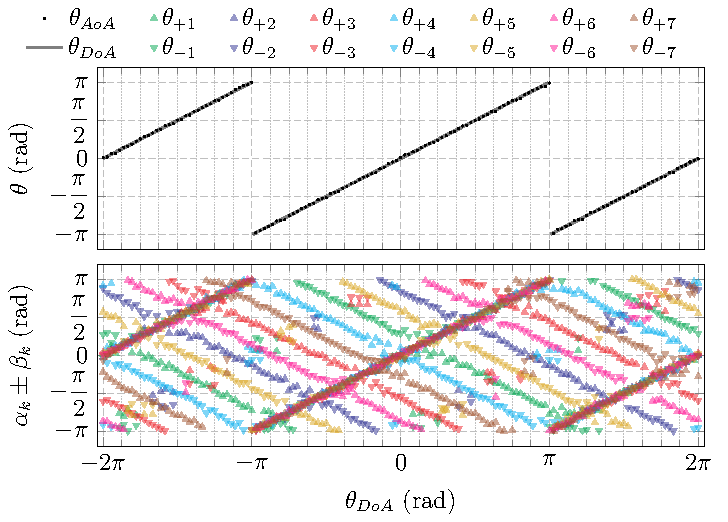
\includegraphics[height=0.785\textheight]{../pictures/simul_POLY_7_R_50_SNR_1_ATT.pdf}
			\caption*{\tiny Fonte: Autor, saída gráfica disponível em \href{https://github.com/HeckRodSav/TG/blob/main/documentation/pictures/POLY_7/simul_POLY_7_R_50_SNR_1_ATT.gif}{\underline{GitHub}}.}
		\end{figure}
	\end{frame}

    \section{Conclusão}

\begin{frame}{Conclusão}
	\begin{itemize}[<+->]\addtolength{\itemsep}{0.5\baselineskip}
		\item É necessário ter uma boa estratégia para localizar um foguete de sondagem;
		\item Para utilizar um GNSS, é necessário decodificar o sinal recebido;
		% \item Se não for possível decodificar, ainda é possível determinar AoA;
		\item Mesmo com o sinal detectável, ainda é possível ter problemas para decodificá-lo;
		\item Analisando a defasagem do sinal entre pares de antenas torna possível estimar o AoA;
		\item Cada par de antenas gera dois possíveis ângulos candidatos;
		\item A proposta utilizando votação se mostrou eficaz.
	\end{itemize}
\end{frame}

\begin{frame}{Conclusão}
	\begin{itemize}[<+->]\addtolength{\itemsep}{0.5\baselineskip}
		\item Dispor as antenas da malha nos vértices de um polígono regular simplificou os cálculos;
		\item Polígonos com quantidade par de lados sempre terão lados paralelos;
		\item Mais pares na malha levaram a maior precisão nos valores obtidos;
		\item O valor mínimo de R\textsuperscript{2} obtido foi superior a \qty{75}{\percent};
		\item O valor médio de R\textsuperscript{2} obtido foi superior a \qty{92}{\percent};
		\item Houveram problemas relacionados ao uso de \textit{software} livre e a manter a compatibilidade entre o GNU Octave e o MATLAB;.
	\end{itemize}
\end{frame}

\begin{frame}{Melhorias futuras}
	\begin{itemize}[<+->]\addtolength{\itemsep}{0.5\baselineskip}
		\item Analisar diferentes disposições de antenas na malha, já que os cálculos não exigem a disposição poligonal;
		\item Contemplar outros tipos de ruído pode acrescentar ao modelo;
		\item Construir um \textit{hardware} capaz de aferir a defasagem em uma malha de antenas poderá contribuir para simulações mais completas.
	\end{itemize}
\end{frame}
    % \input{../slides/Z_outtro}

    \section{Finalização}
    \begin{frame}
        \begin{center}
            \VERYHuge \usebeamercolor[fg]{title}\textbf{Perguntas?}
        \end{center}
    \end{frame}

    \begin{frame}
        \begin{center}
            \VERYHuge \usebeamercolor[fg]{title}\textbf{Obrigado!}
        \end{center}
    \end{frame}

\end{document}
